% Generated by scripts/plot_xyz_spline_summaries_linear.py.
\clearpage
\subsubsection{dQ/dx}
\begin{figure}[H]
\centering
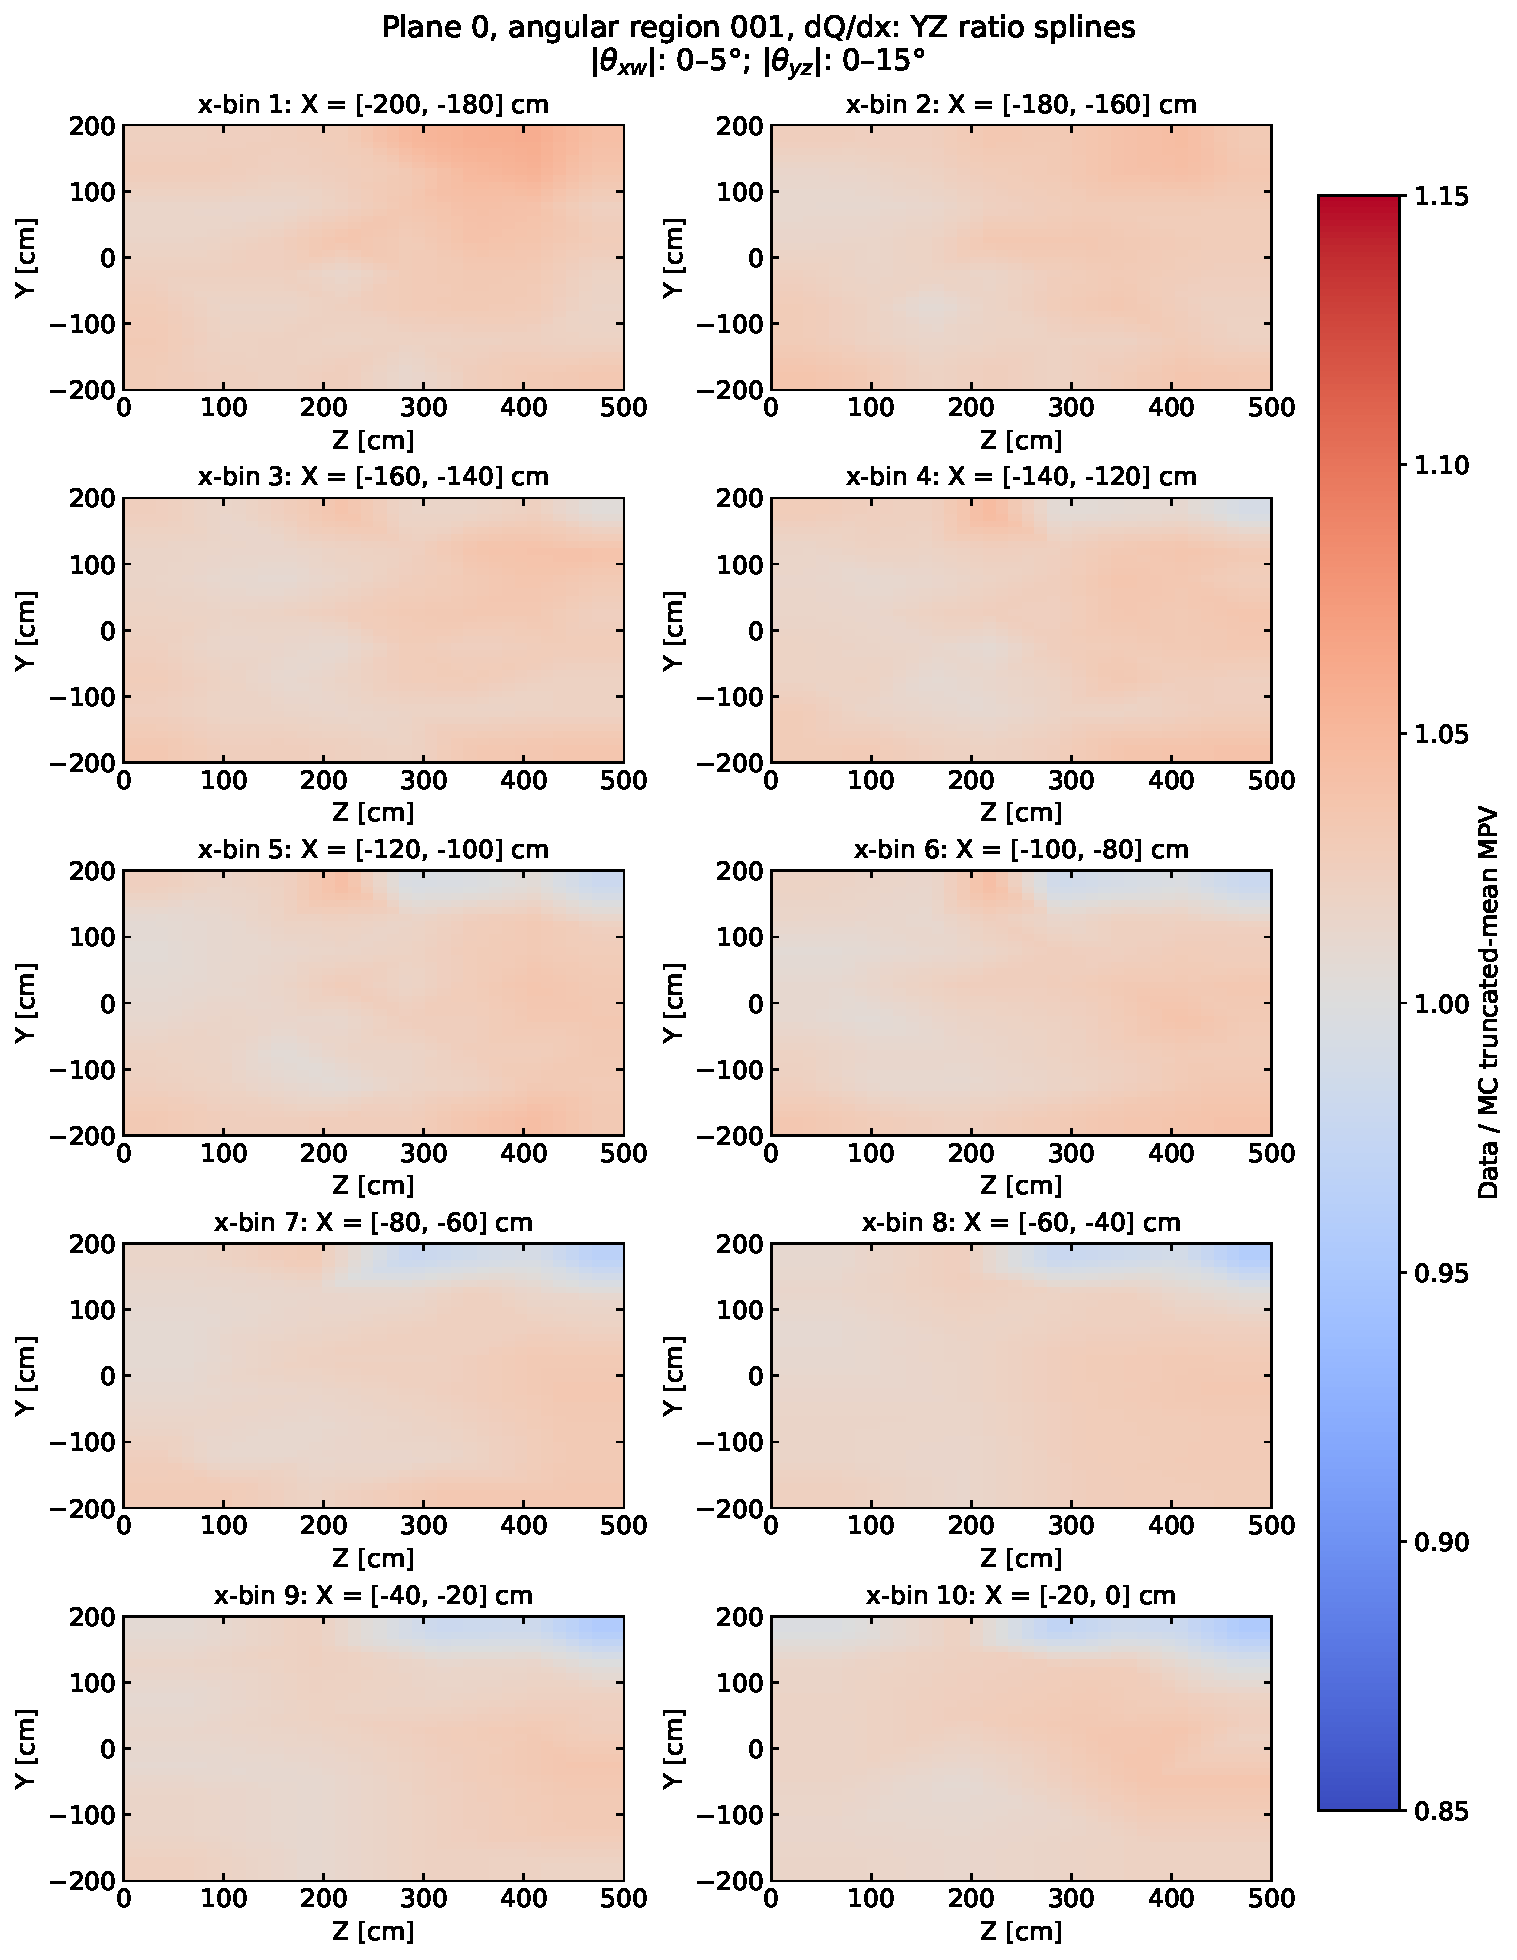
\includegraphics[width=\textwidth,height=0.80\textheight,keepaspectratio]{Figures/WireModXYZ/summary/plane0/anglebin_dq_plane0_region001_xyz_ratio_spline_summary_linear.pdf}
\caption{Plane 0, angular region 001: dQ/dx YZ data/MC ratio surfaces for all populated x-bins. The folded angular selection is $|\theta_{xw}|\in[0,5]^\circ$ and $|\theta_{yz}|\in[0,15]^\circ$.}
\label{fig:xyz_linear_dq_plane0_region001}
\end{figure}

\clearpage
\begin{figure}[H]
\centering
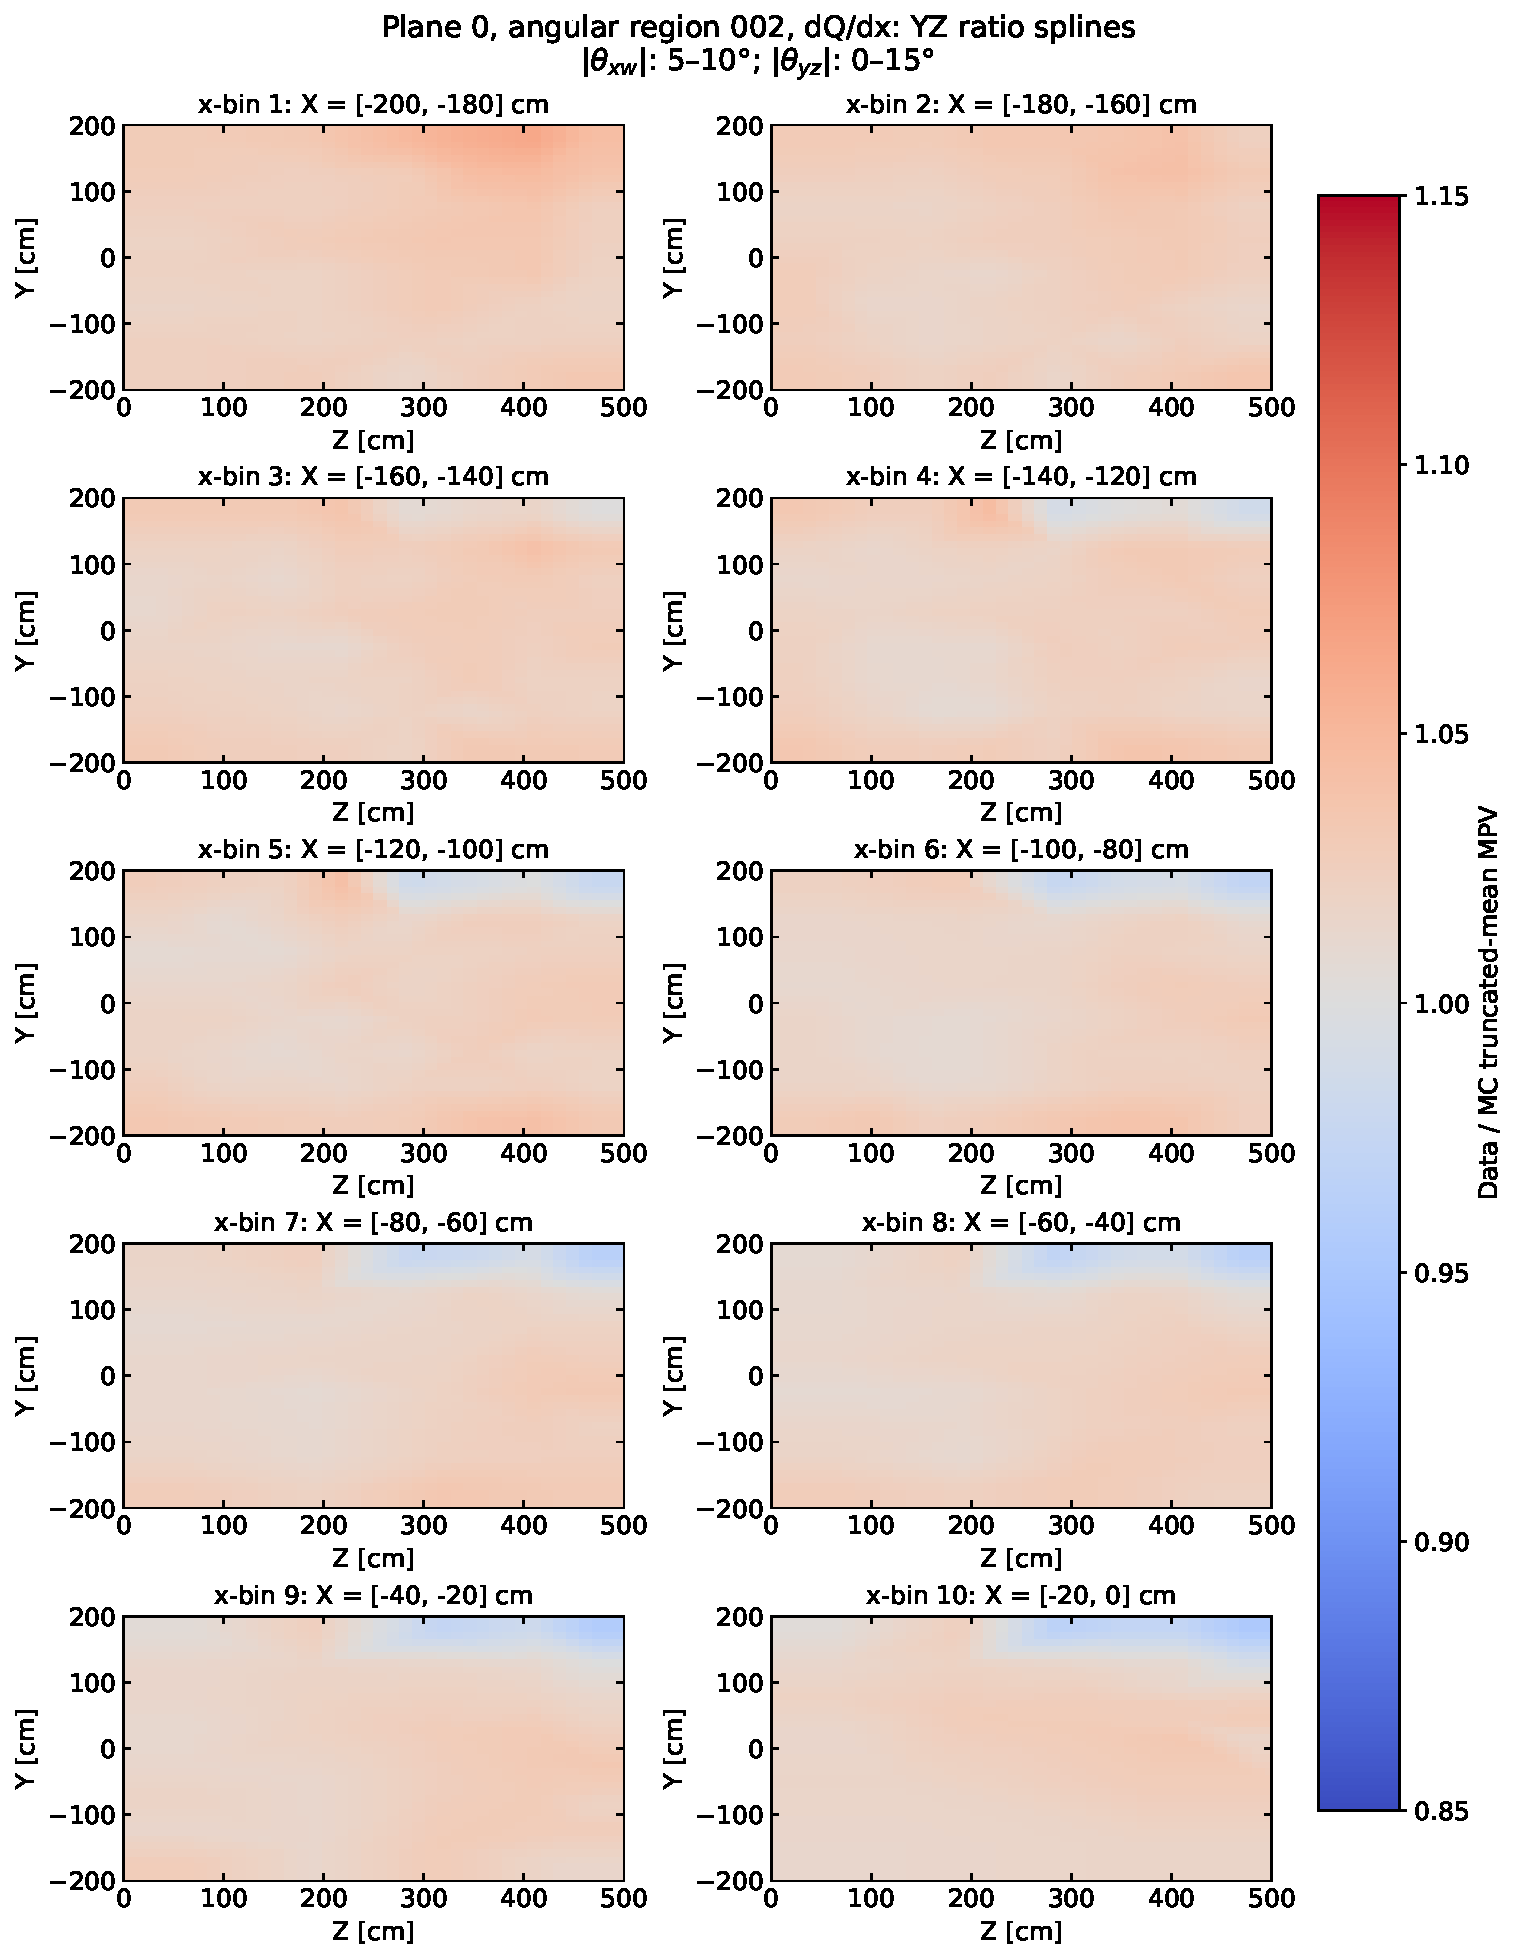
\includegraphics[width=\textwidth,height=0.80\textheight,keepaspectratio]{Figures/WireModXYZ/summary/plane0/anglebin_dq_plane0_region002_xyz_ratio_spline_summary_linear.pdf}
\caption{Plane 0, angular region 002: dQ/dx YZ data/MC ratio surfaces for all populated x-bins. The folded angular selection is $|\theta_{xw}|\in[5,10]^\circ$ and $|\theta_{yz}|\in[0,15]^\circ$.}
\label{fig:xyz_linear_dq_plane0_region002}
\end{figure}

\clearpage
\begin{figure}[H]
\centering
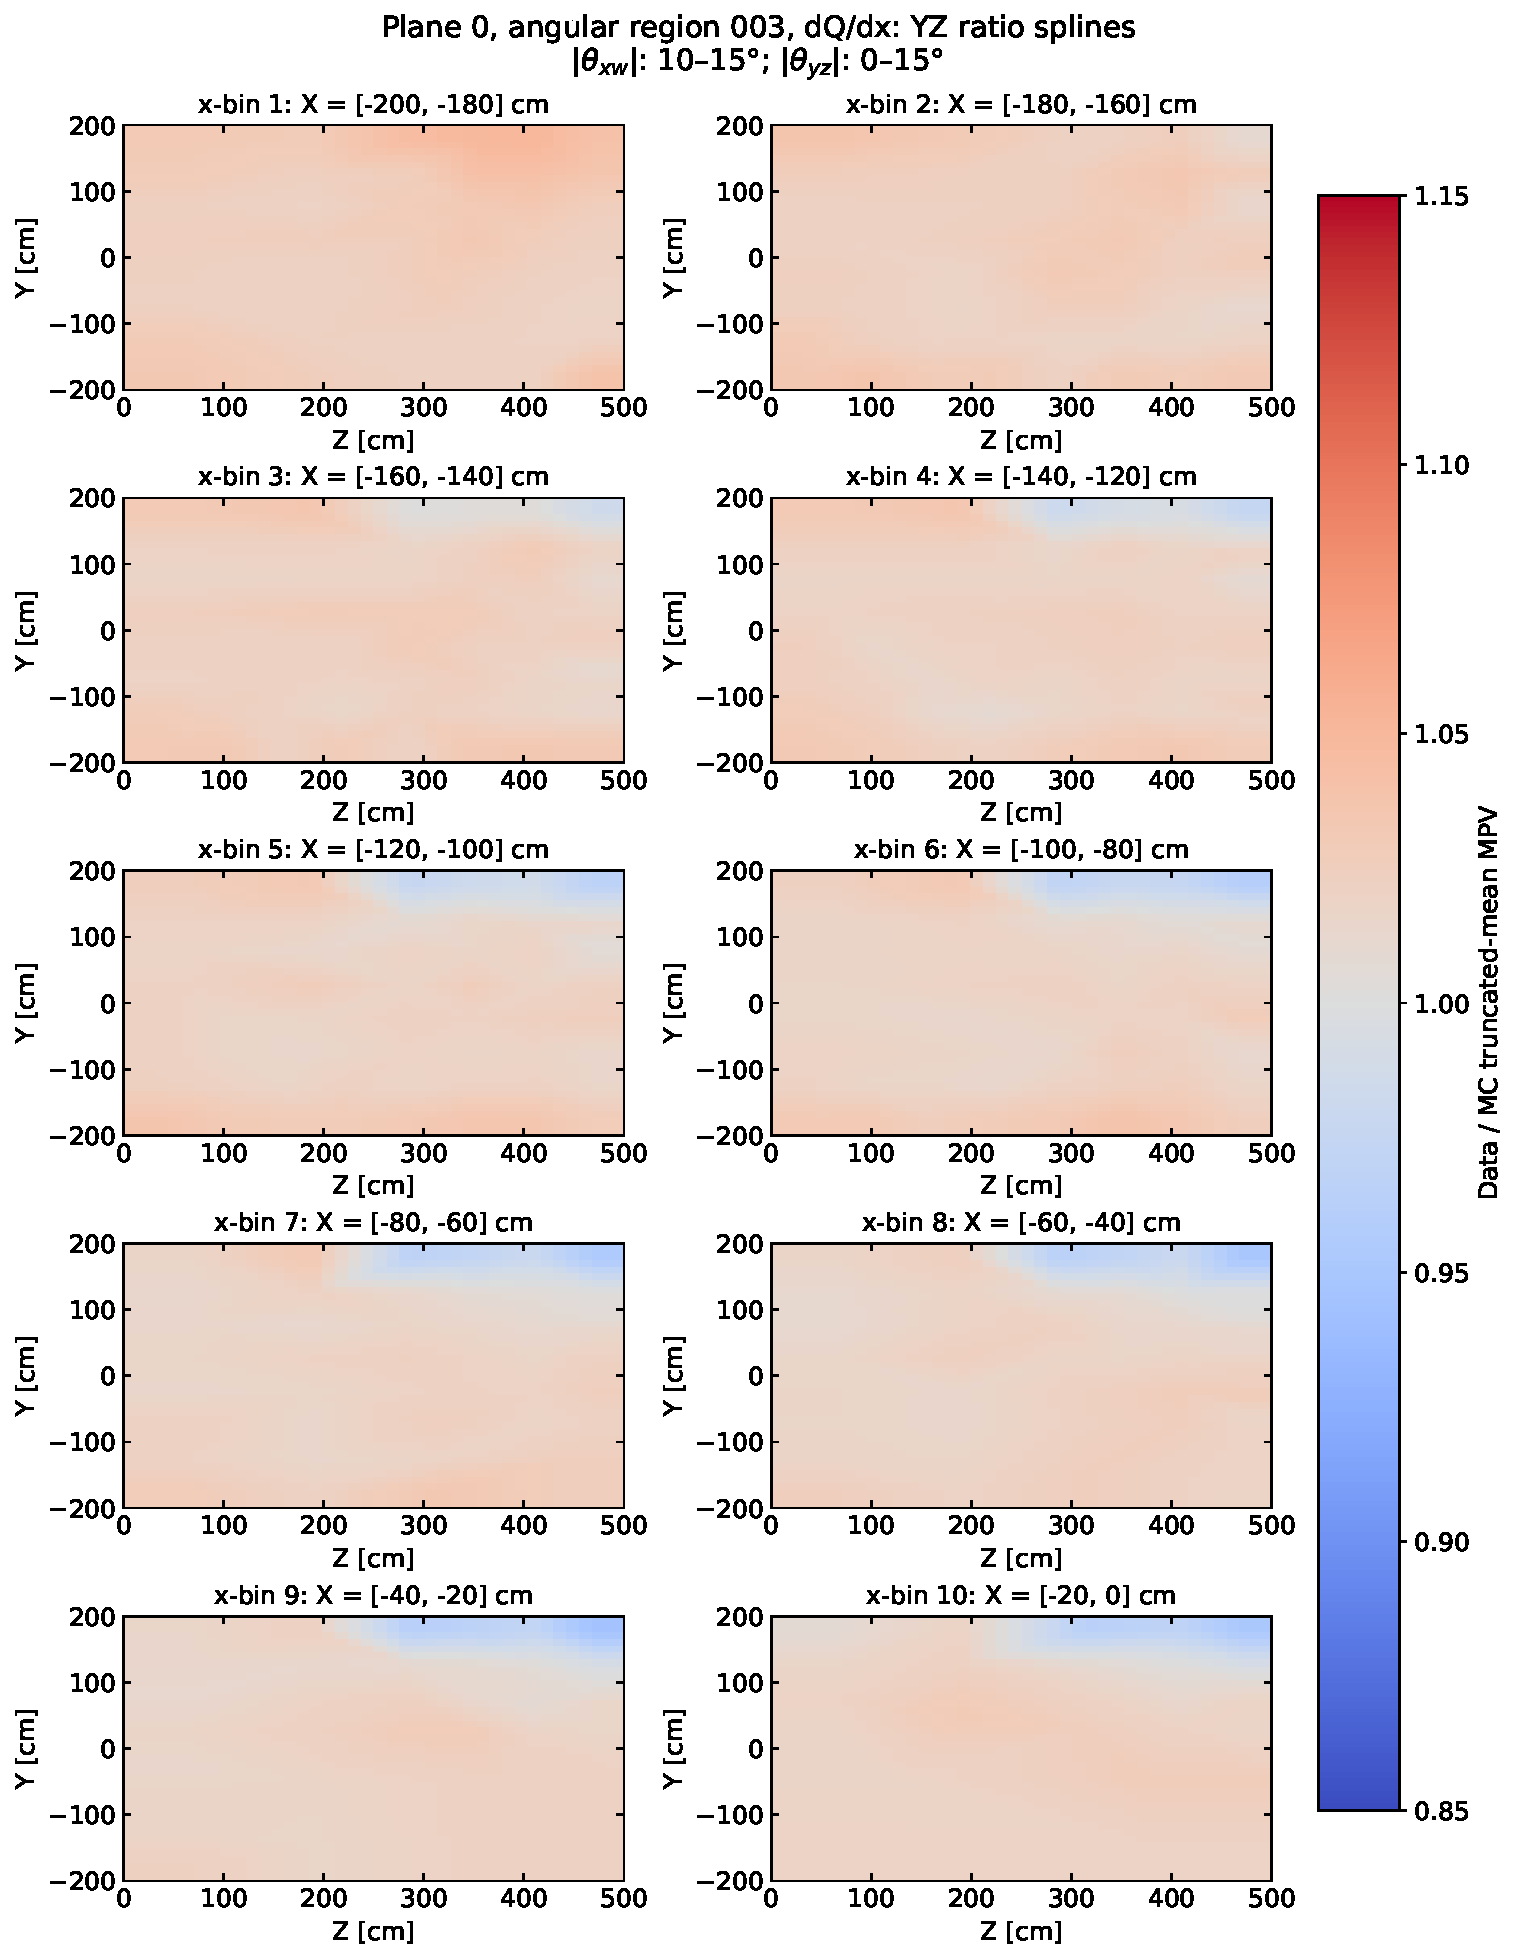
\includegraphics[width=\textwidth,height=0.80\textheight,keepaspectratio]{Figures/WireModXYZ/summary/plane0/anglebin_dq_plane0_region003_xyz_ratio_spline_summary_linear.pdf}
\caption{Plane 0, angular region 003: dQ/dx YZ data/MC ratio surfaces for all populated x-bins. The folded angular selection is $|\theta_{xw}|\in[10,15]^\circ$ and $|\theta_{yz}|\in[0,15]^\circ$.}
\label{fig:xyz_linear_dq_plane0_region003}
\end{figure}

\clearpage
\begin{figure}[H]
\centering
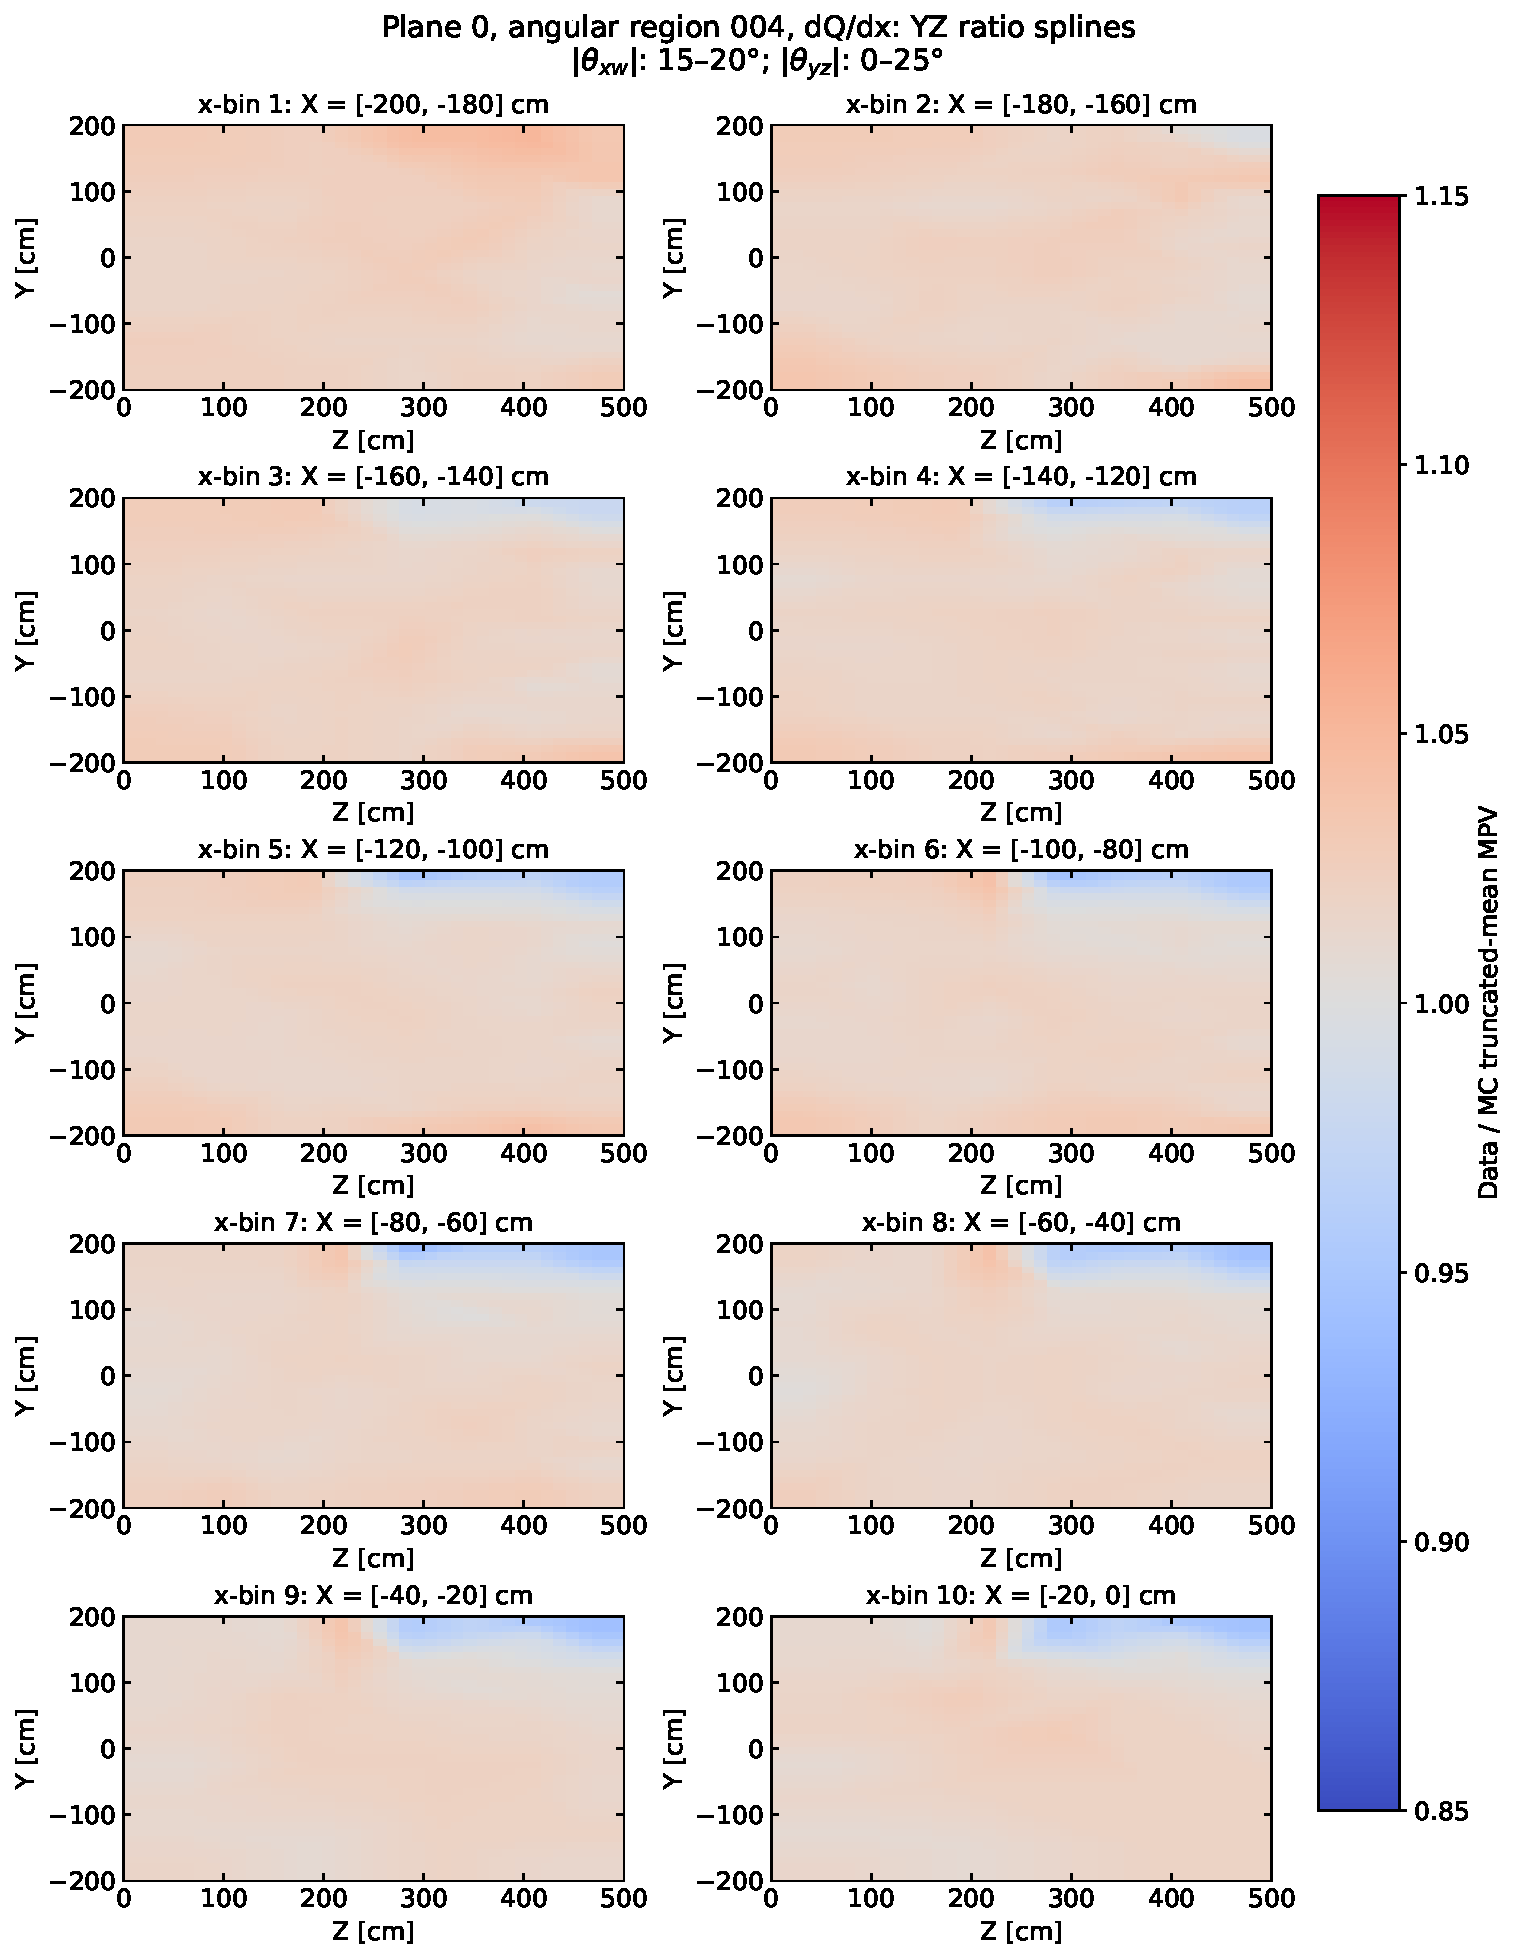
\includegraphics[width=\textwidth,height=0.80\textheight,keepaspectratio]{Figures/WireModXYZ/summary/plane0/anglebin_dq_plane0_region004_xyz_ratio_spline_summary_linear.pdf}
\caption{Plane 0, angular region 004: dQ/dx YZ data/MC ratio surfaces for all populated x-bins. The folded angular selection is $|\theta_{xw}|\in[15,20]^\circ$ and $|\theta_{yz}|\in[0,25]^\circ$.}
\label{fig:xyz_linear_dq_plane0_region004}
\end{figure}

\clearpage
\begin{figure}[H]
\centering
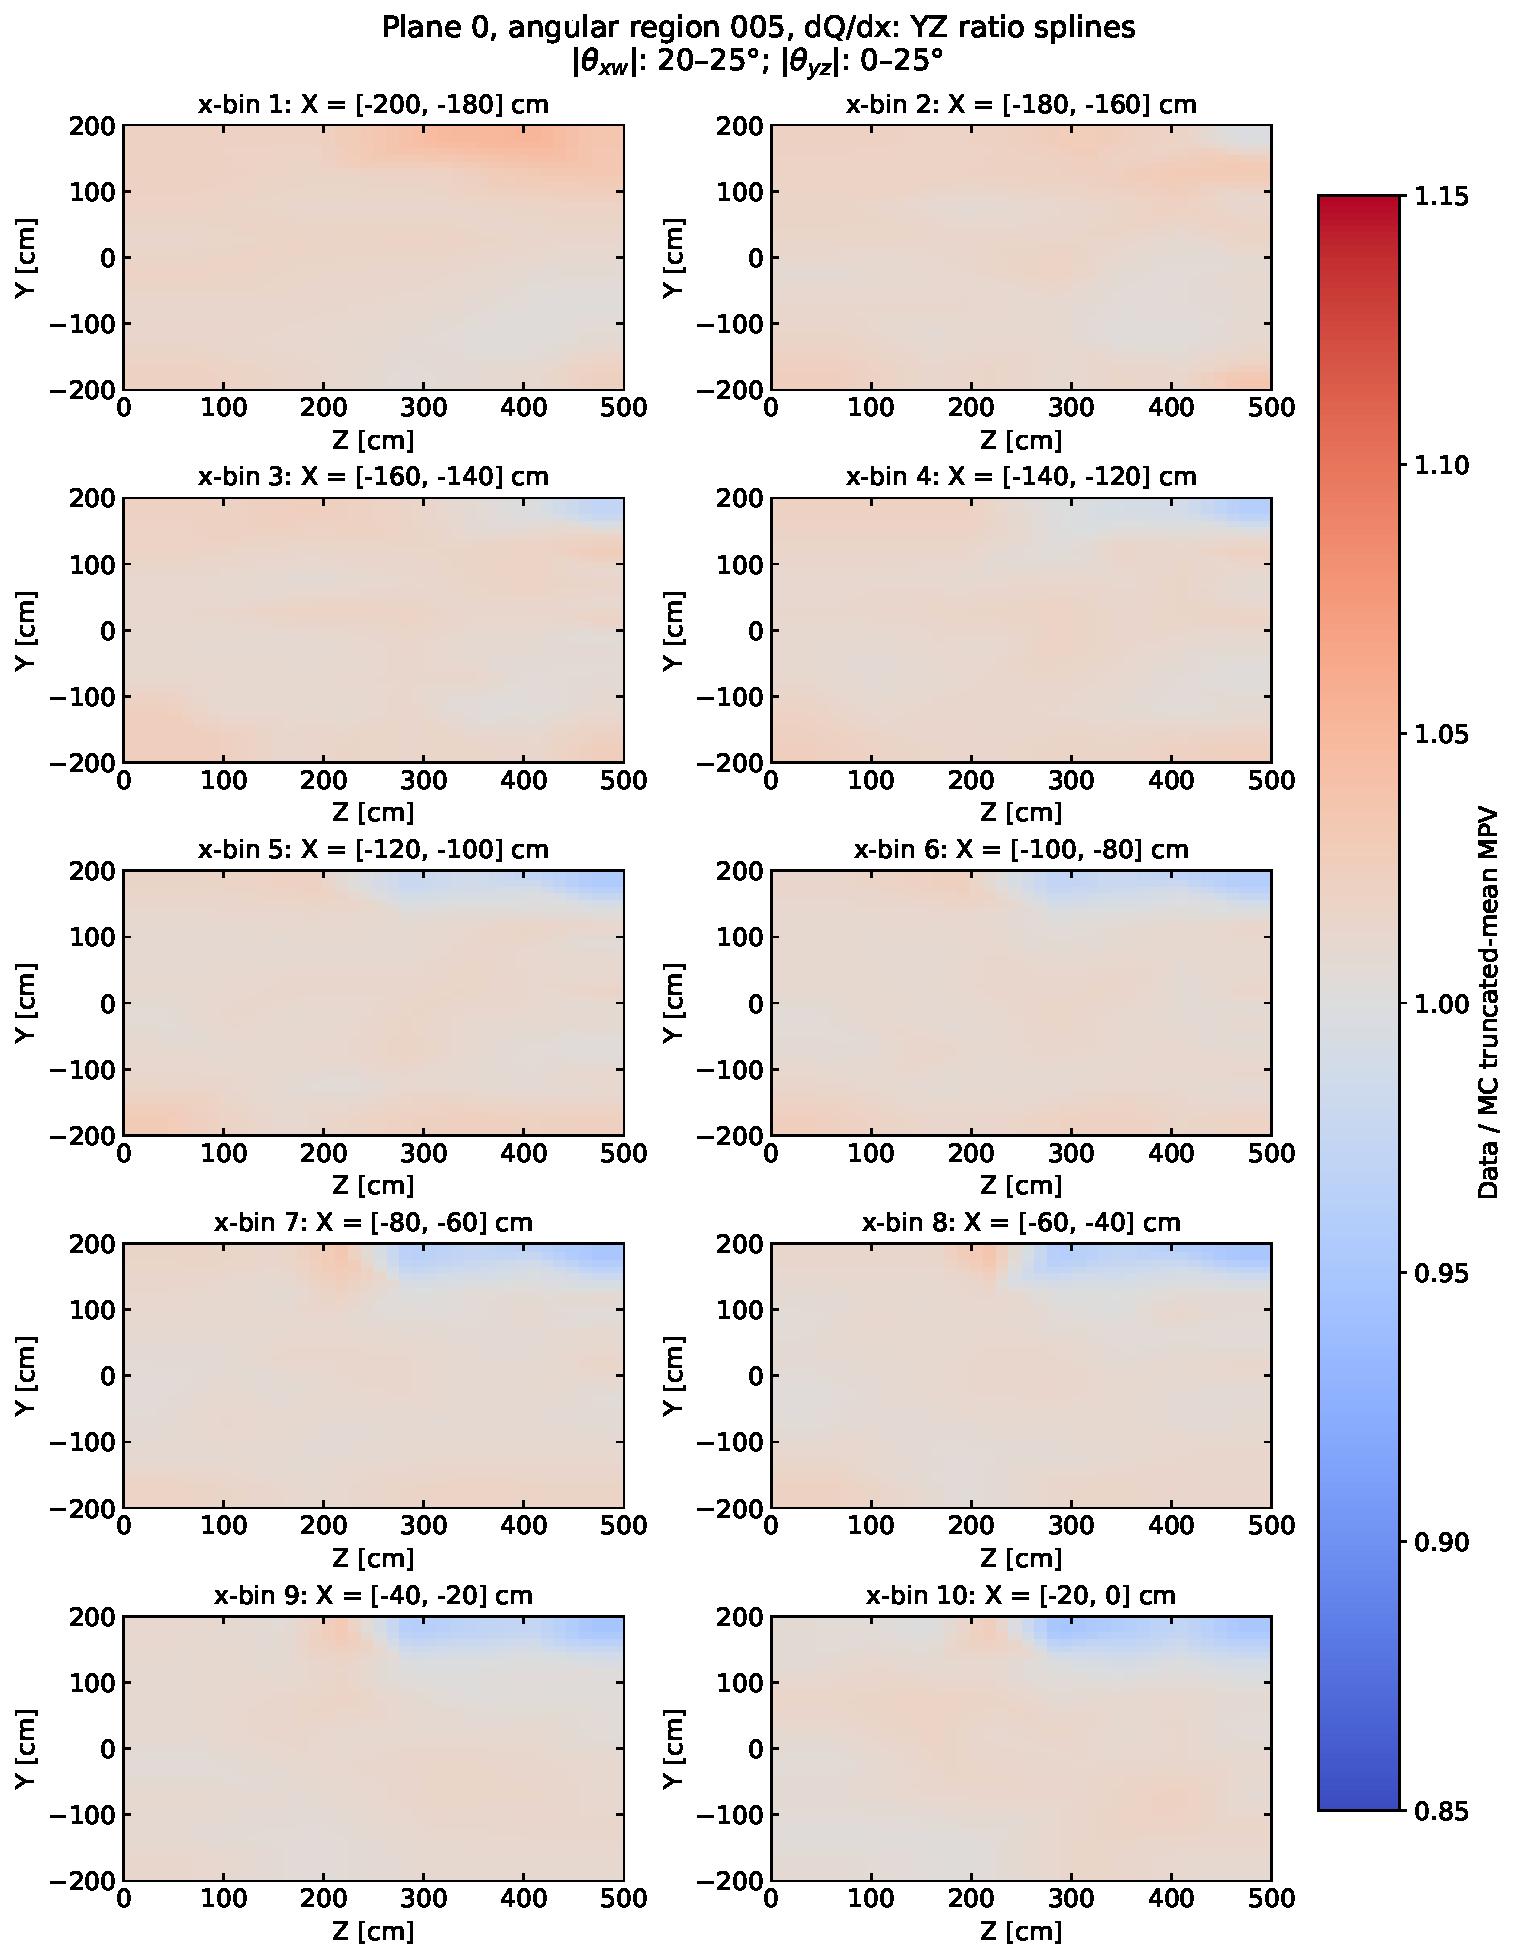
\includegraphics[width=\textwidth,height=0.80\textheight,keepaspectratio]{Figures/WireModXYZ/summary/plane0/anglebin_dq_plane0_region005_xyz_ratio_spline_summary_linear.pdf}
\caption{Plane 0, angular region 005: dQ/dx YZ data/MC ratio surfaces for all populated x-bins. The folded angular selection is $|\theta_{xw}|\in[20,25]^\circ$ and $|\theta_{yz}|\in[0,25]^\circ$.}
\label{fig:xyz_linear_dq_plane0_region005}
\end{figure}

\clearpage
\begin{figure}[H]
\centering
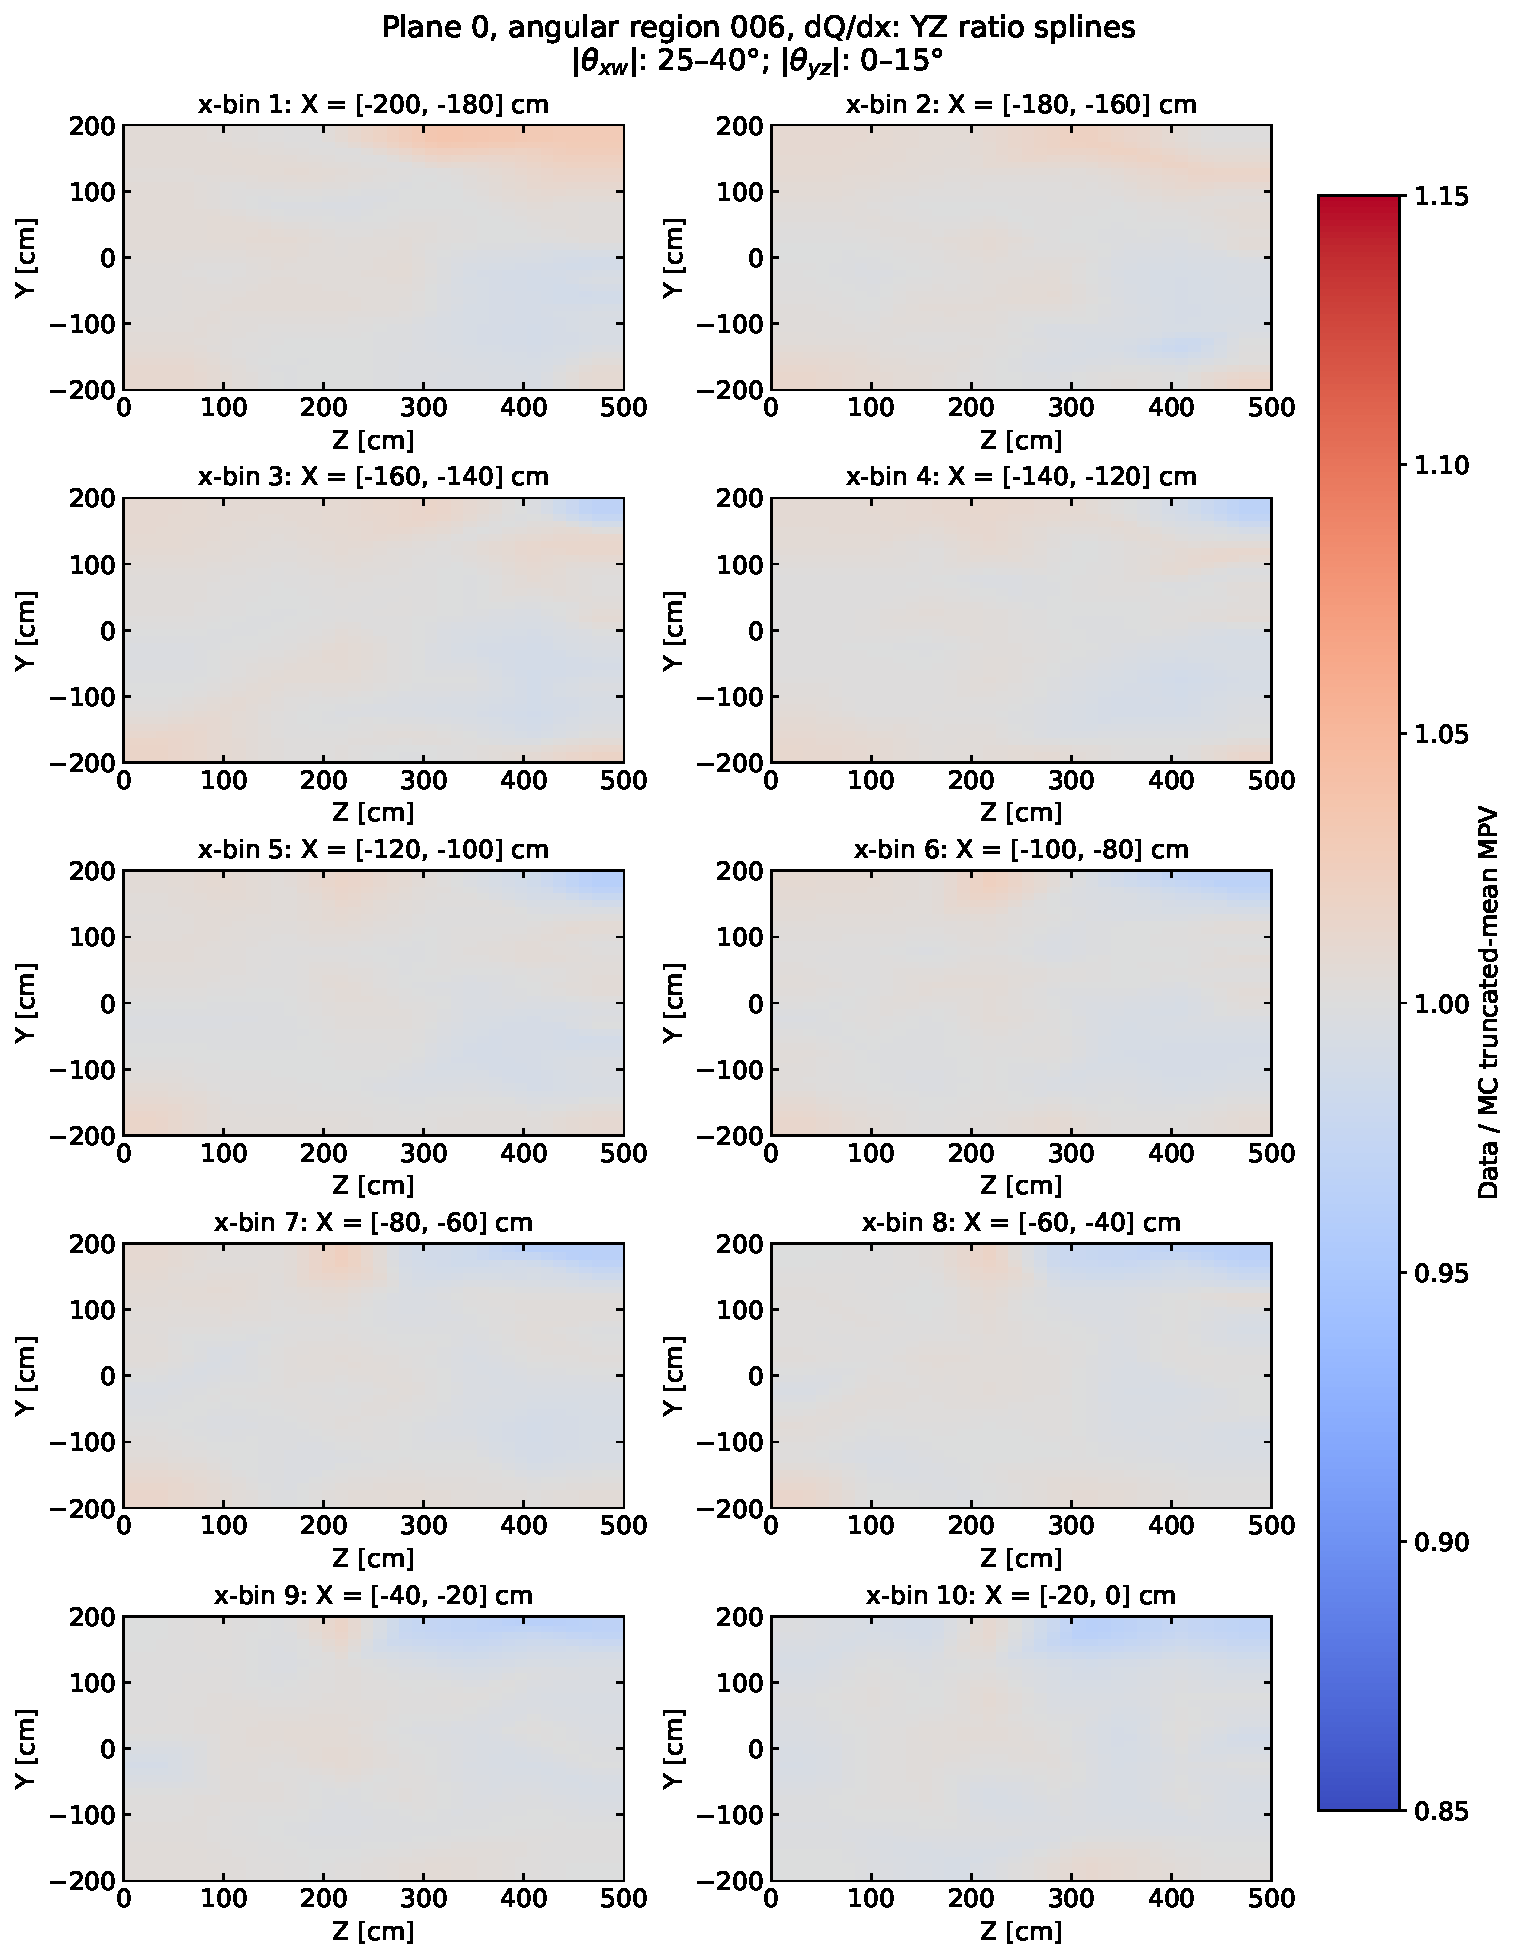
\includegraphics[width=\textwidth,height=0.80\textheight,keepaspectratio]{Figures/WireModXYZ/summary/plane0/anglebin_dq_plane0_region006_xyz_ratio_spline_summary_linear.pdf}
\caption{Plane 0, angular region 006: dQ/dx YZ data/MC ratio surfaces for all populated x-bins. The folded angular selection is $|\theta_{xw}|\in[25,40]^\circ$ and $|\theta_{yz}|\in[0,15]^\circ$.}
\label{fig:xyz_linear_dq_plane0_region006}
\end{figure}

\clearpage
\begin{figure}[H]
\centering
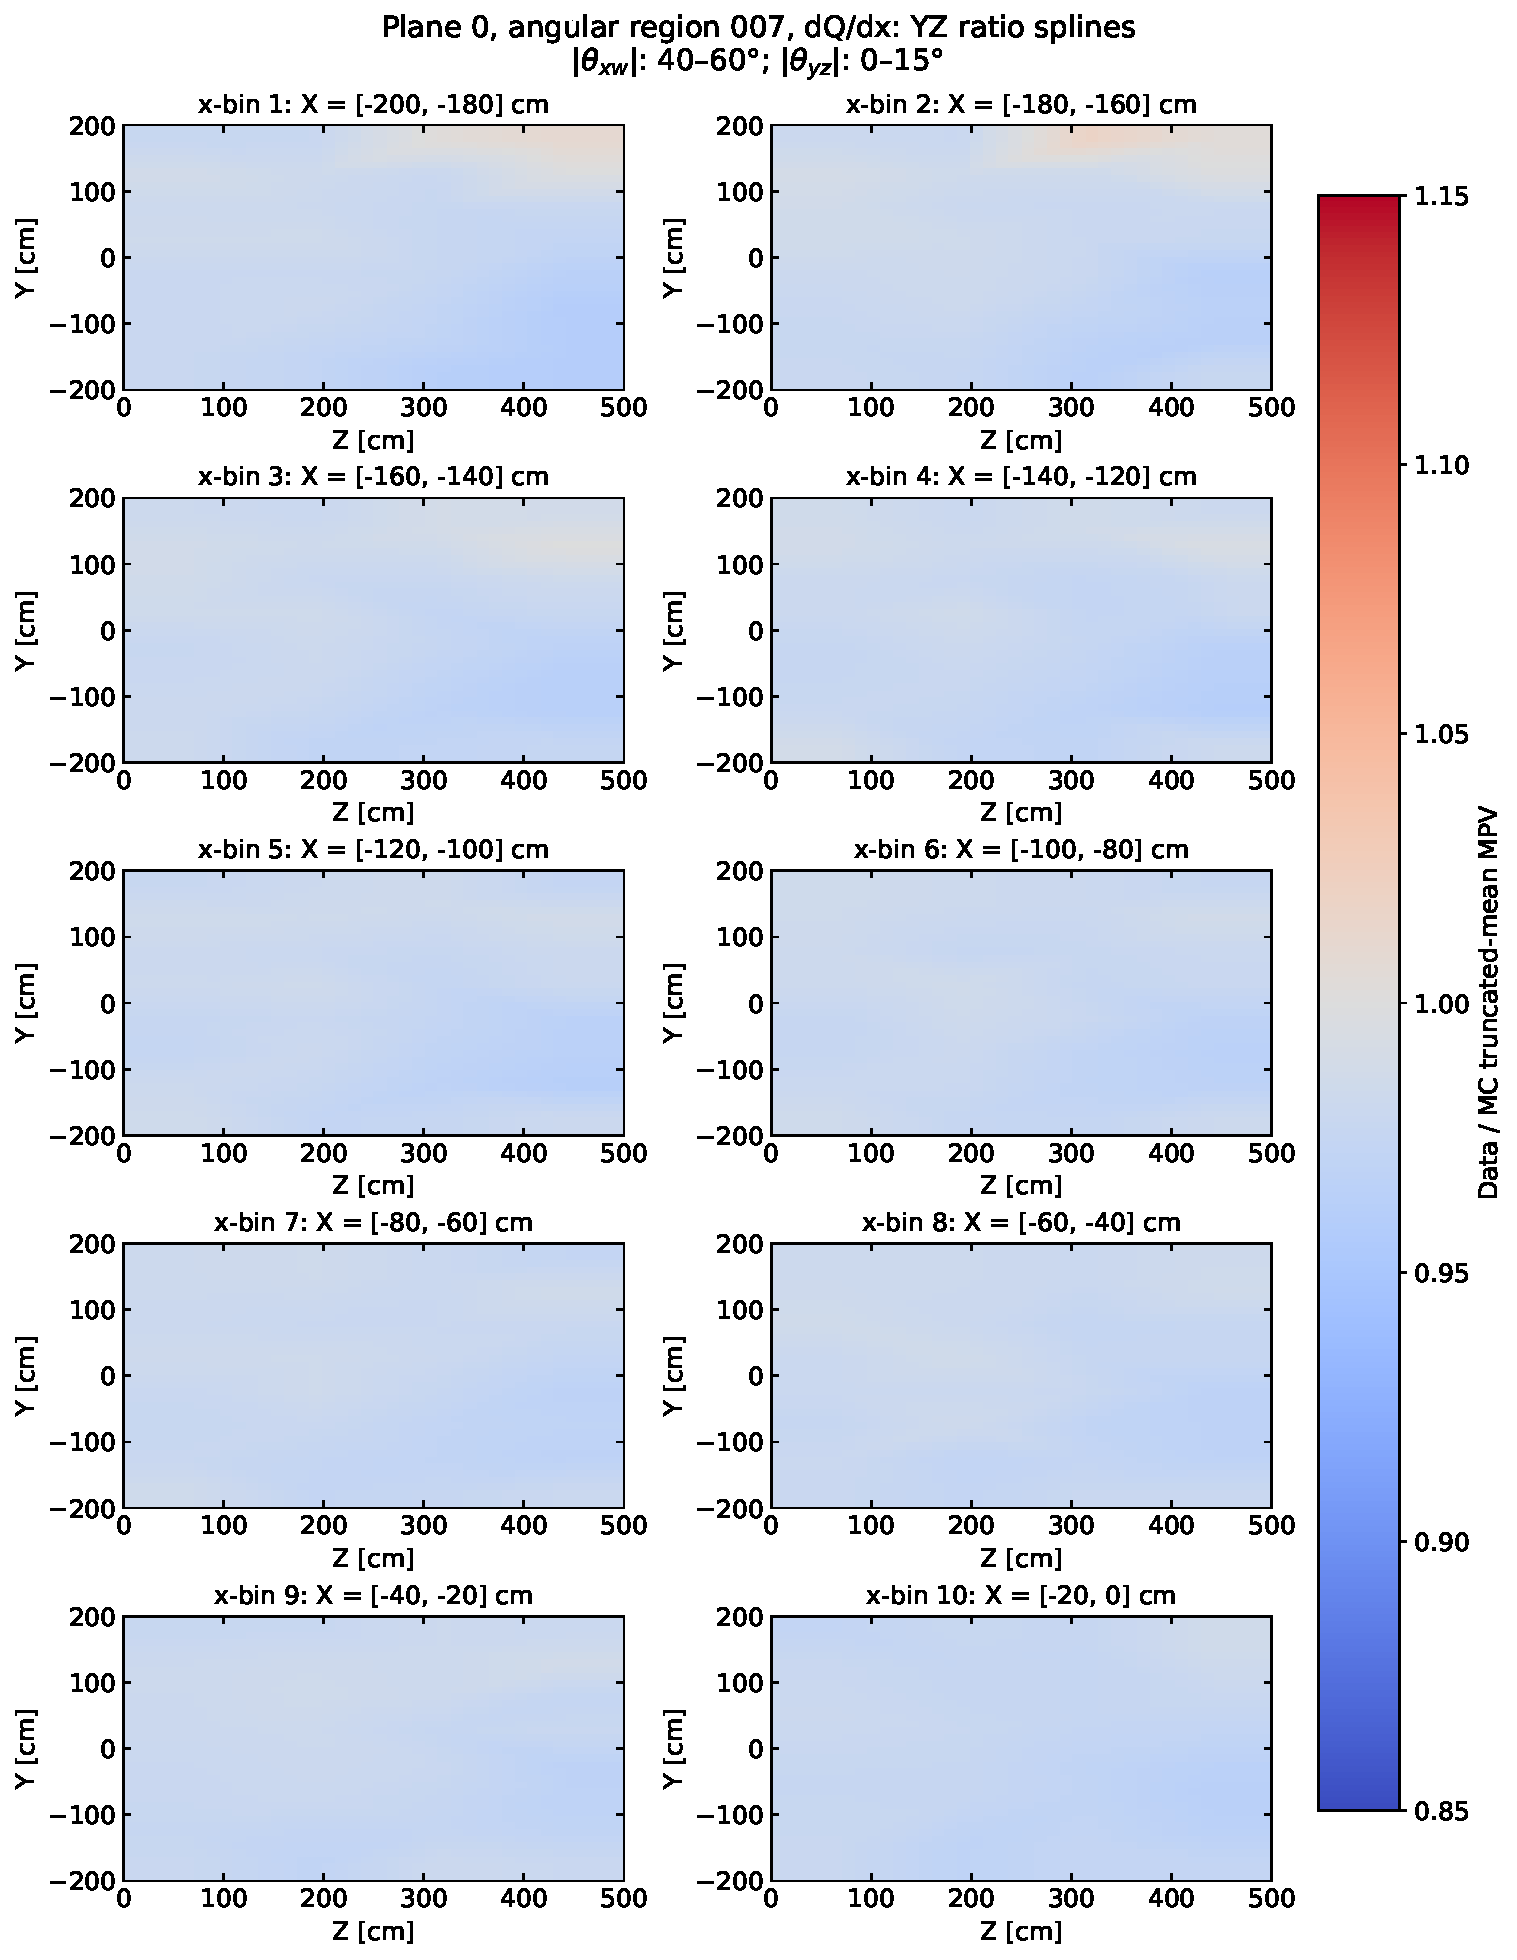
\includegraphics[width=\textwidth,height=0.80\textheight,keepaspectratio]{Figures/WireModXYZ/summary/plane0/anglebin_dq_plane0_region007_xyz_ratio_spline_summary_linear.pdf}
\caption{Plane 0, angular region 007: dQ/dx YZ data/MC ratio surfaces for all populated x-bins. The folded angular selection is $|\theta_{xw}|\in[40,60]^\circ$ and $|\theta_{yz}|\in[0,15]^\circ$.}
\label{fig:xyz_linear_dq_plane0_region007}
\end{figure}

\clearpage
\begin{figure}[H]
\centering
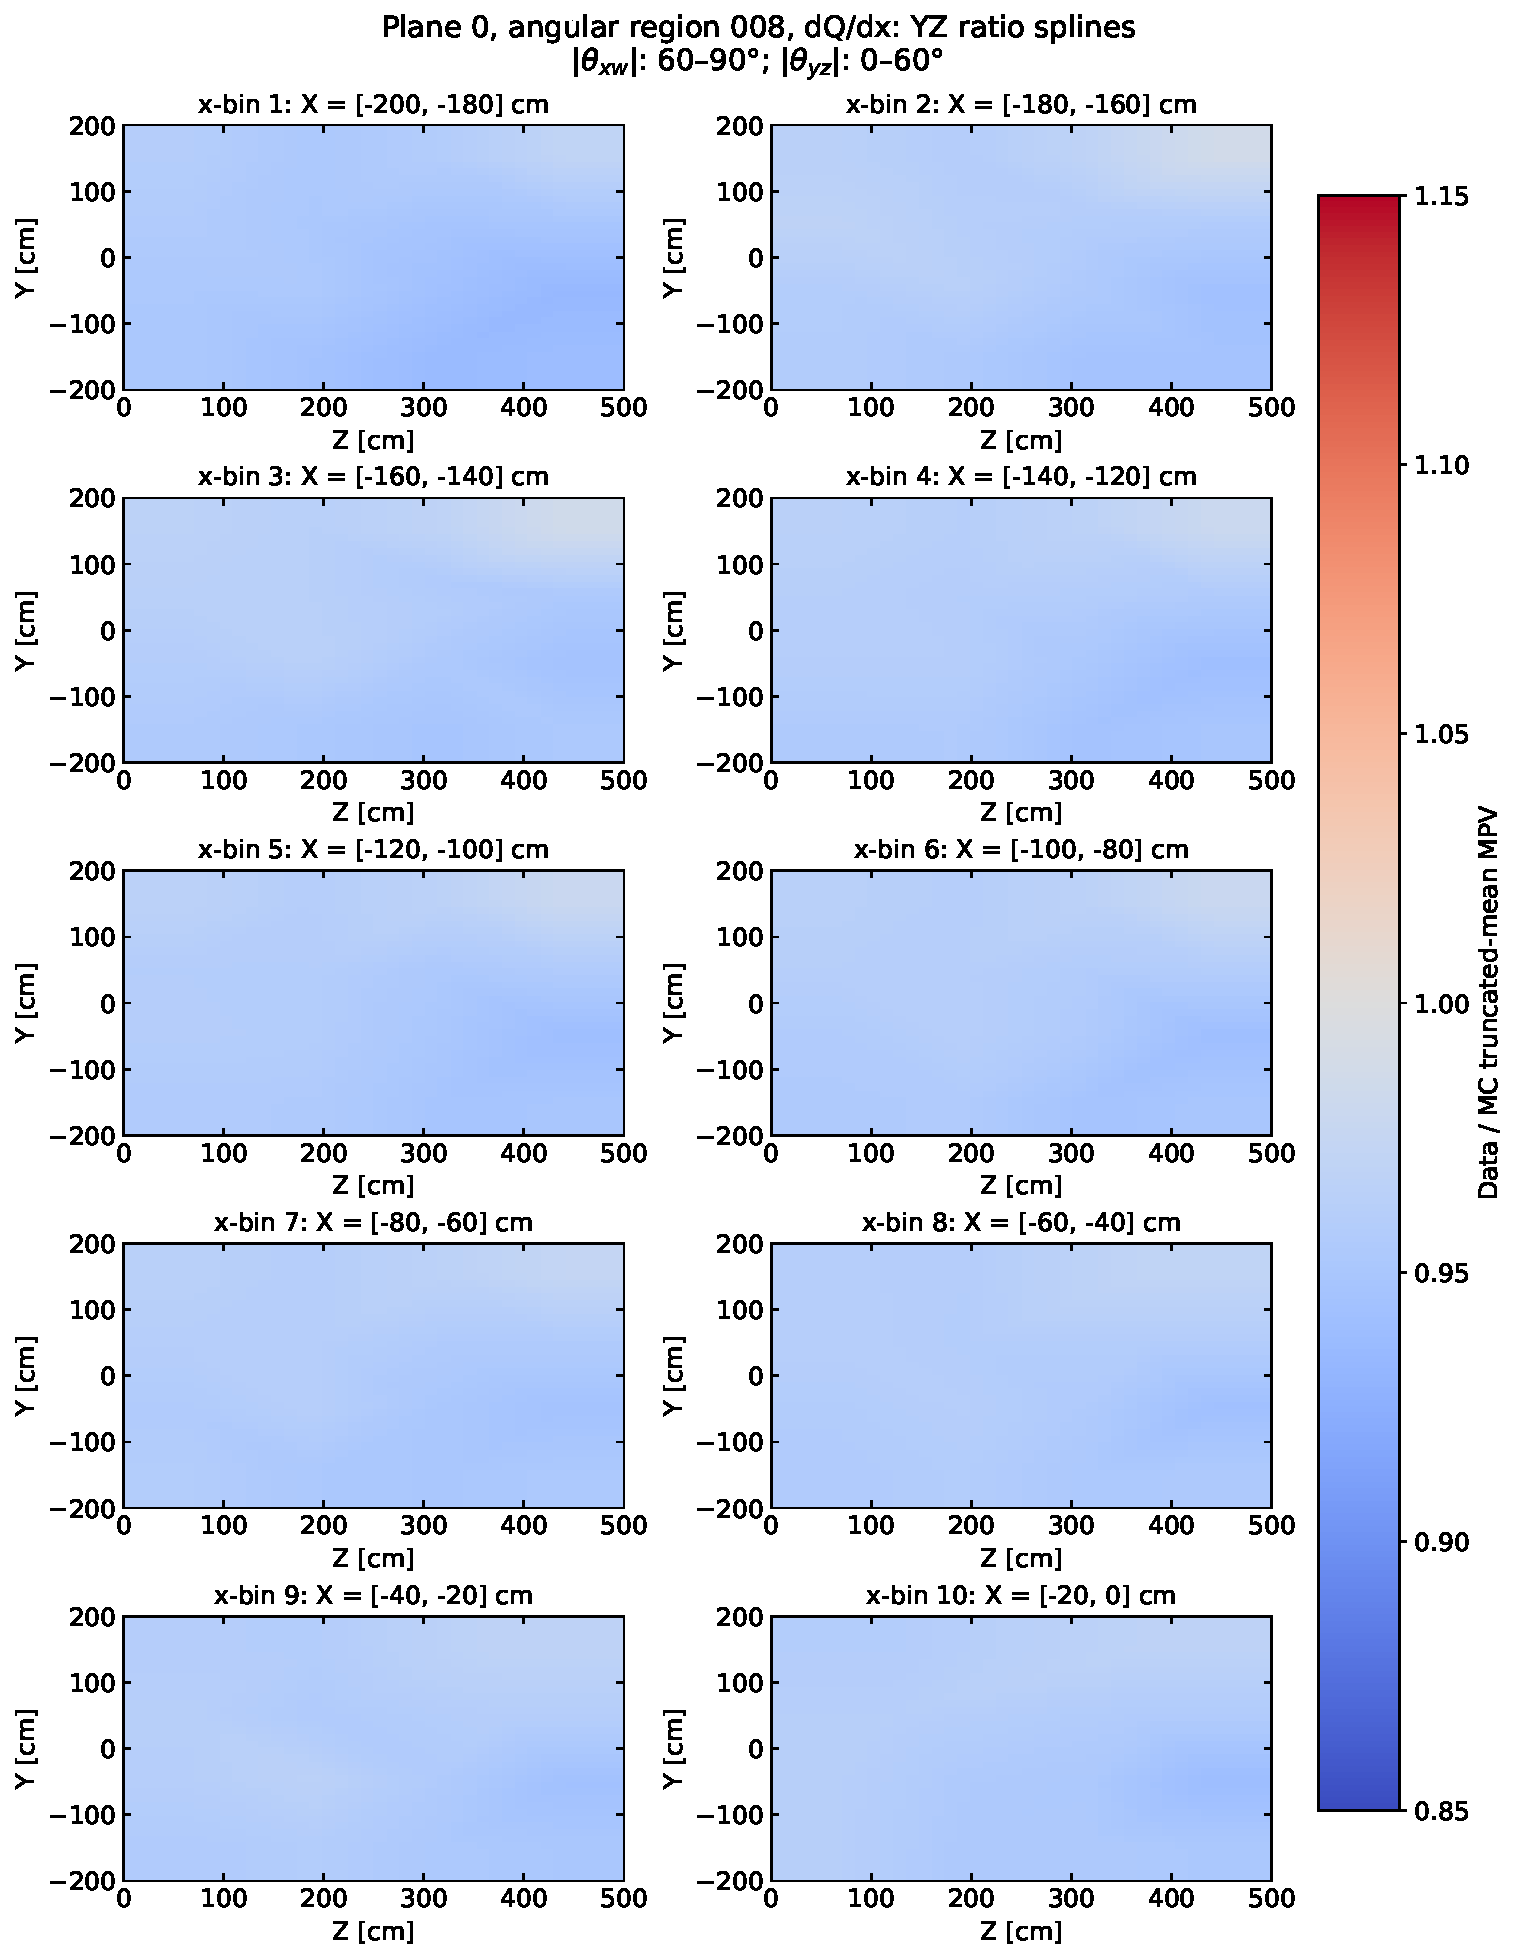
\includegraphics[width=\textwidth,height=0.80\textheight,keepaspectratio]{Figures/WireModXYZ/summary/plane0/anglebin_dq_plane0_region008_xyz_ratio_spline_summary_linear.pdf}
\caption{Plane 0, angular region 008: dQ/dx YZ data/MC ratio surfaces for all populated x-bins. The folded angular selection is $|\theta_{xw}|\in[60,90]^\circ$ and $|\theta_{yz}|\in[0,60]^\circ$.}
\label{fig:xyz_linear_dq_plane0_region008}
\end{figure}

\clearpage
\begin{figure}[H]
\centering
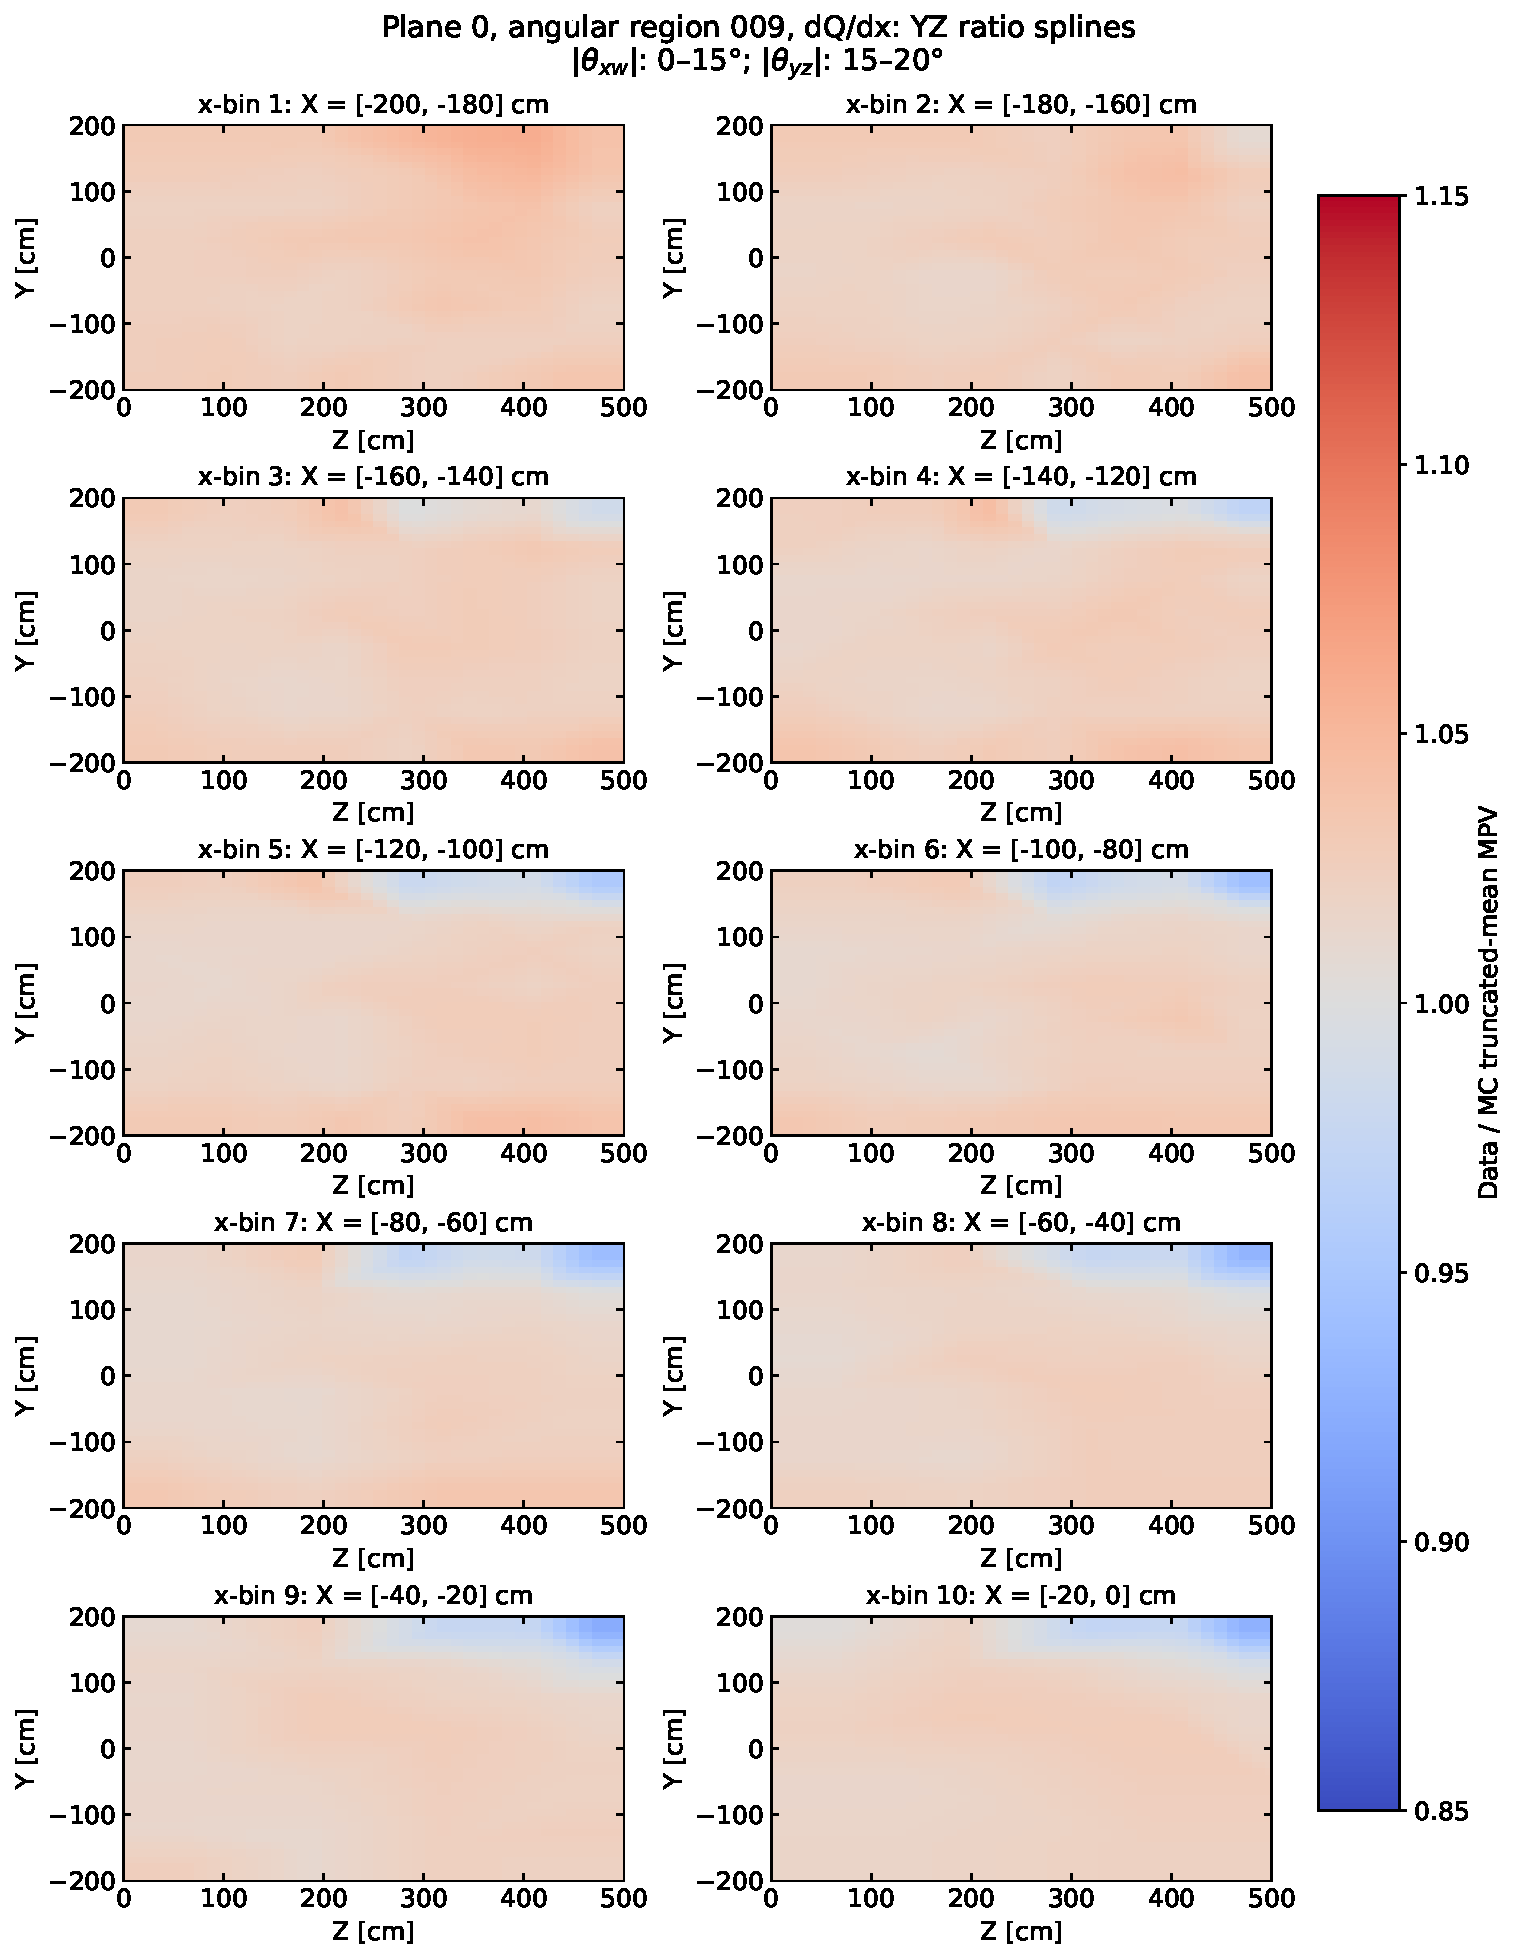
\includegraphics[width=\textwidth,height=0.80\textheight,keepaspectratio]{Figures/WireModXYZ/summary/plane0/anglebin_dq_plane0_region009_xyz_ratio_spline_summary_linear.pdf}
\caption{Plane 0, angular region 009: dQ/dx YZ data/MC ratio surfaces for all populated x-bins. The folded angular selection is $|\theta_{xw}|\in[0,15]^\circ$ and $|\theta_{yz}|\in[15,20]^\circ$.}
\label{fig:xyz_linear_dq_plane0_region009}
\end{figure}

\clearpage
\begin{figure}[H]
\centering
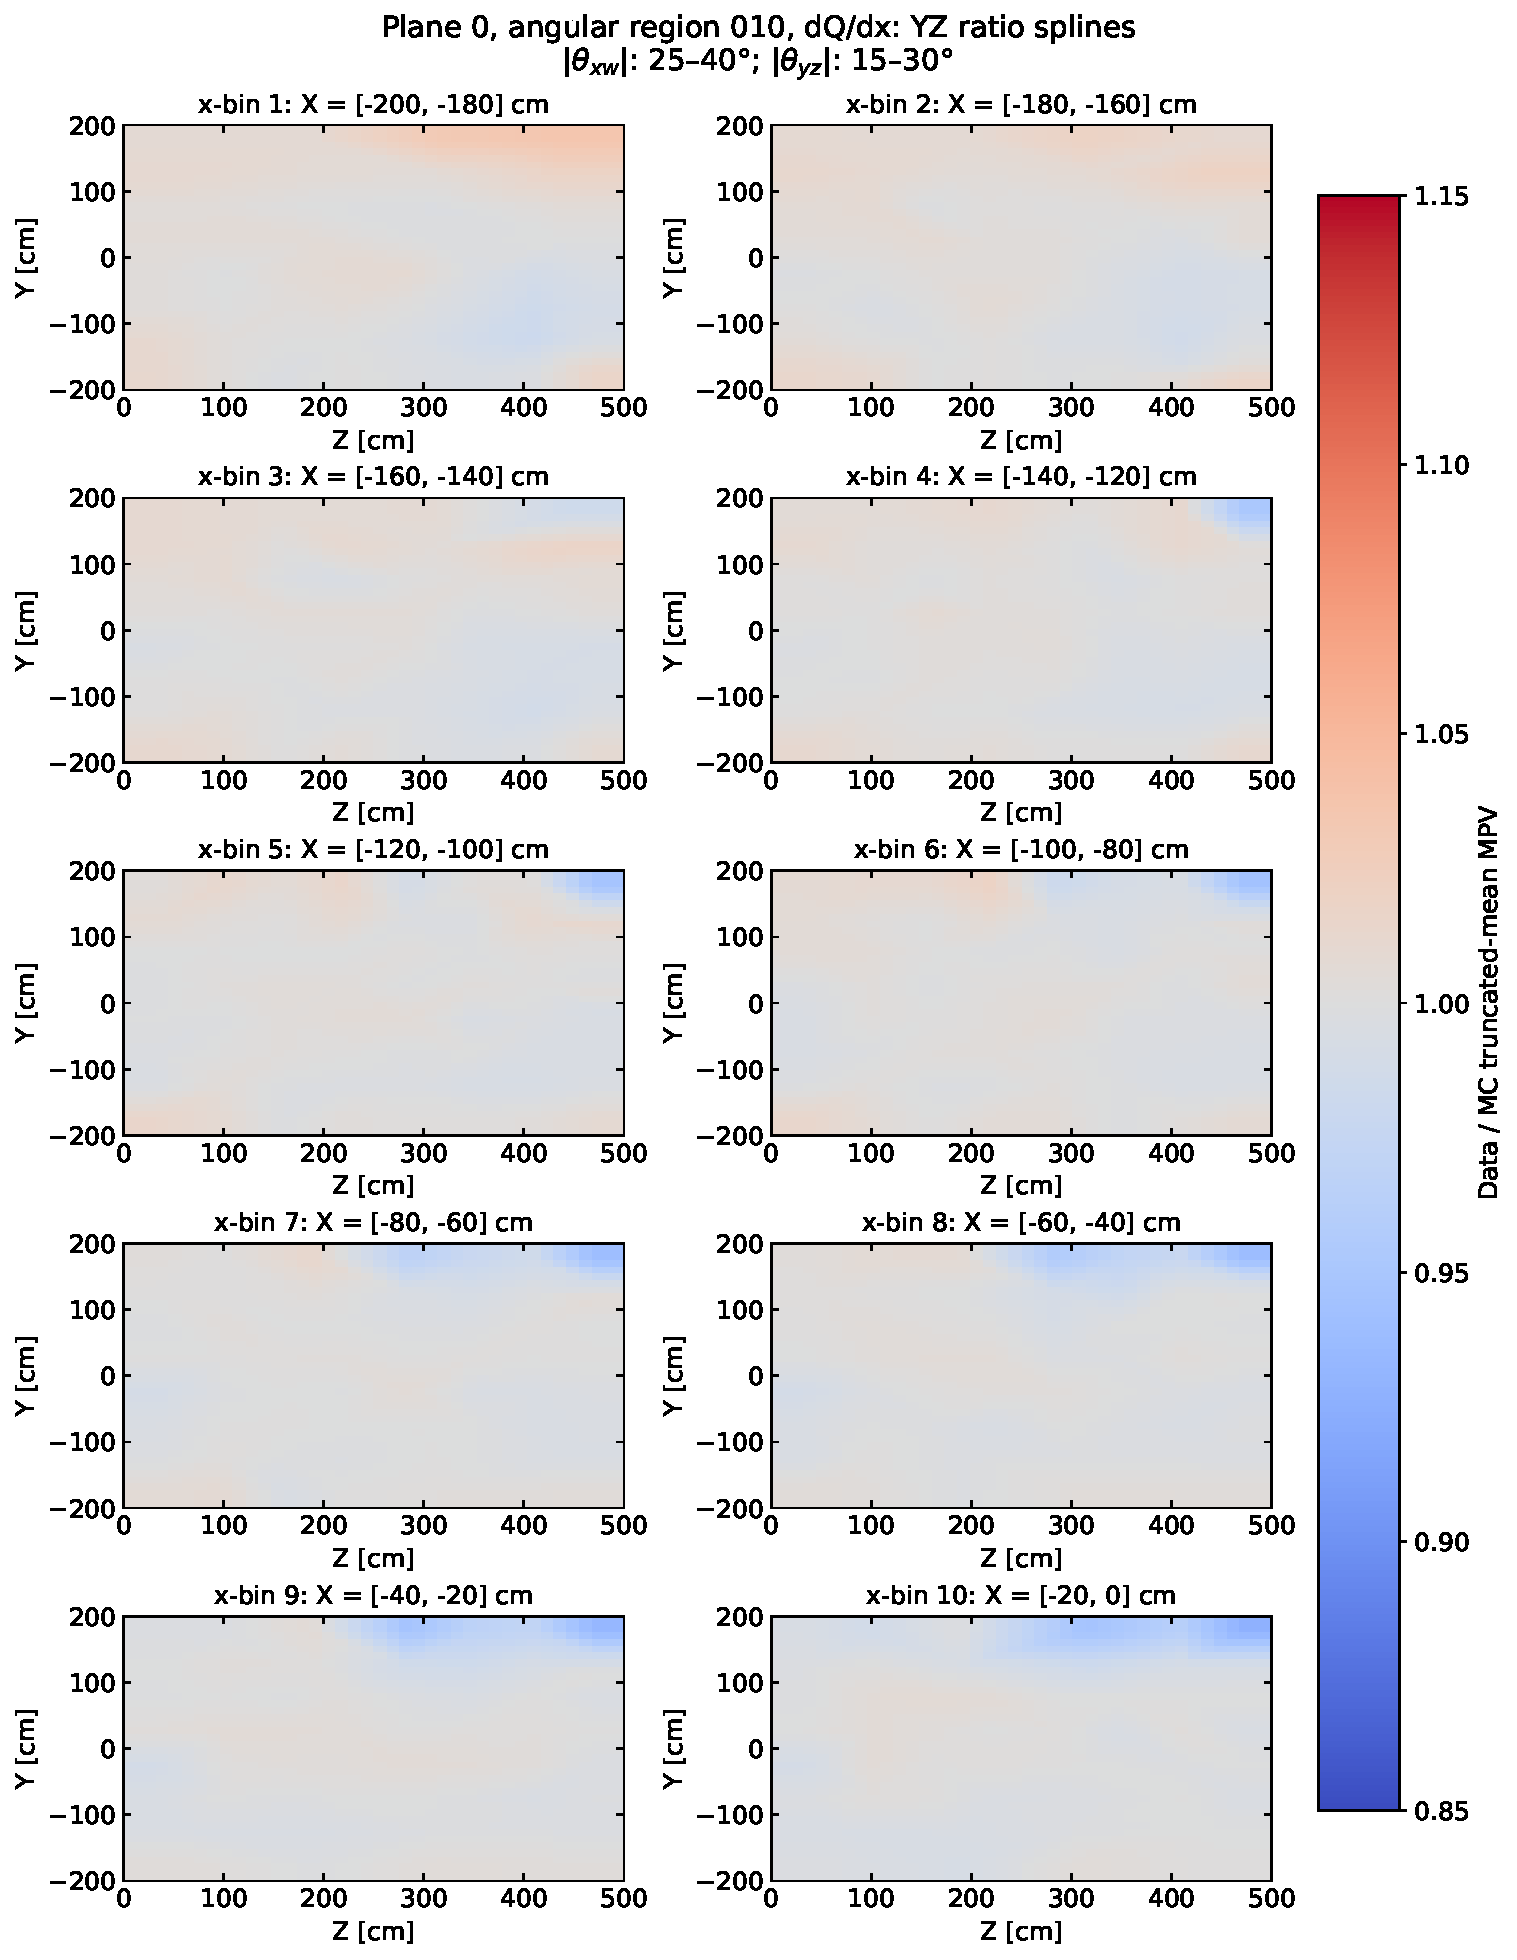
\includegraphics[width=\textwidth,height=0.80\textheight,keepaspectratio]{Figures/WireModXYZ/summary/plane0/anglebin_dq_plane0_region010_xyz_ratio_spline_summary_linear.pdf}
\caption{Plane 0, angular region 010: dQ/dx YZ data/MC ratio surfaces for all populated x-bins. The folded angular selection is $|\theta_{xw}|\in[25,40]^\circ$ and $|\theta_{yz}|\in[15,30]^\circ$.}
\label{fig:xyz_linear_dq_plane0_region010}
\end{figure}

\clearpage
\begin{figure}[H]
\centering
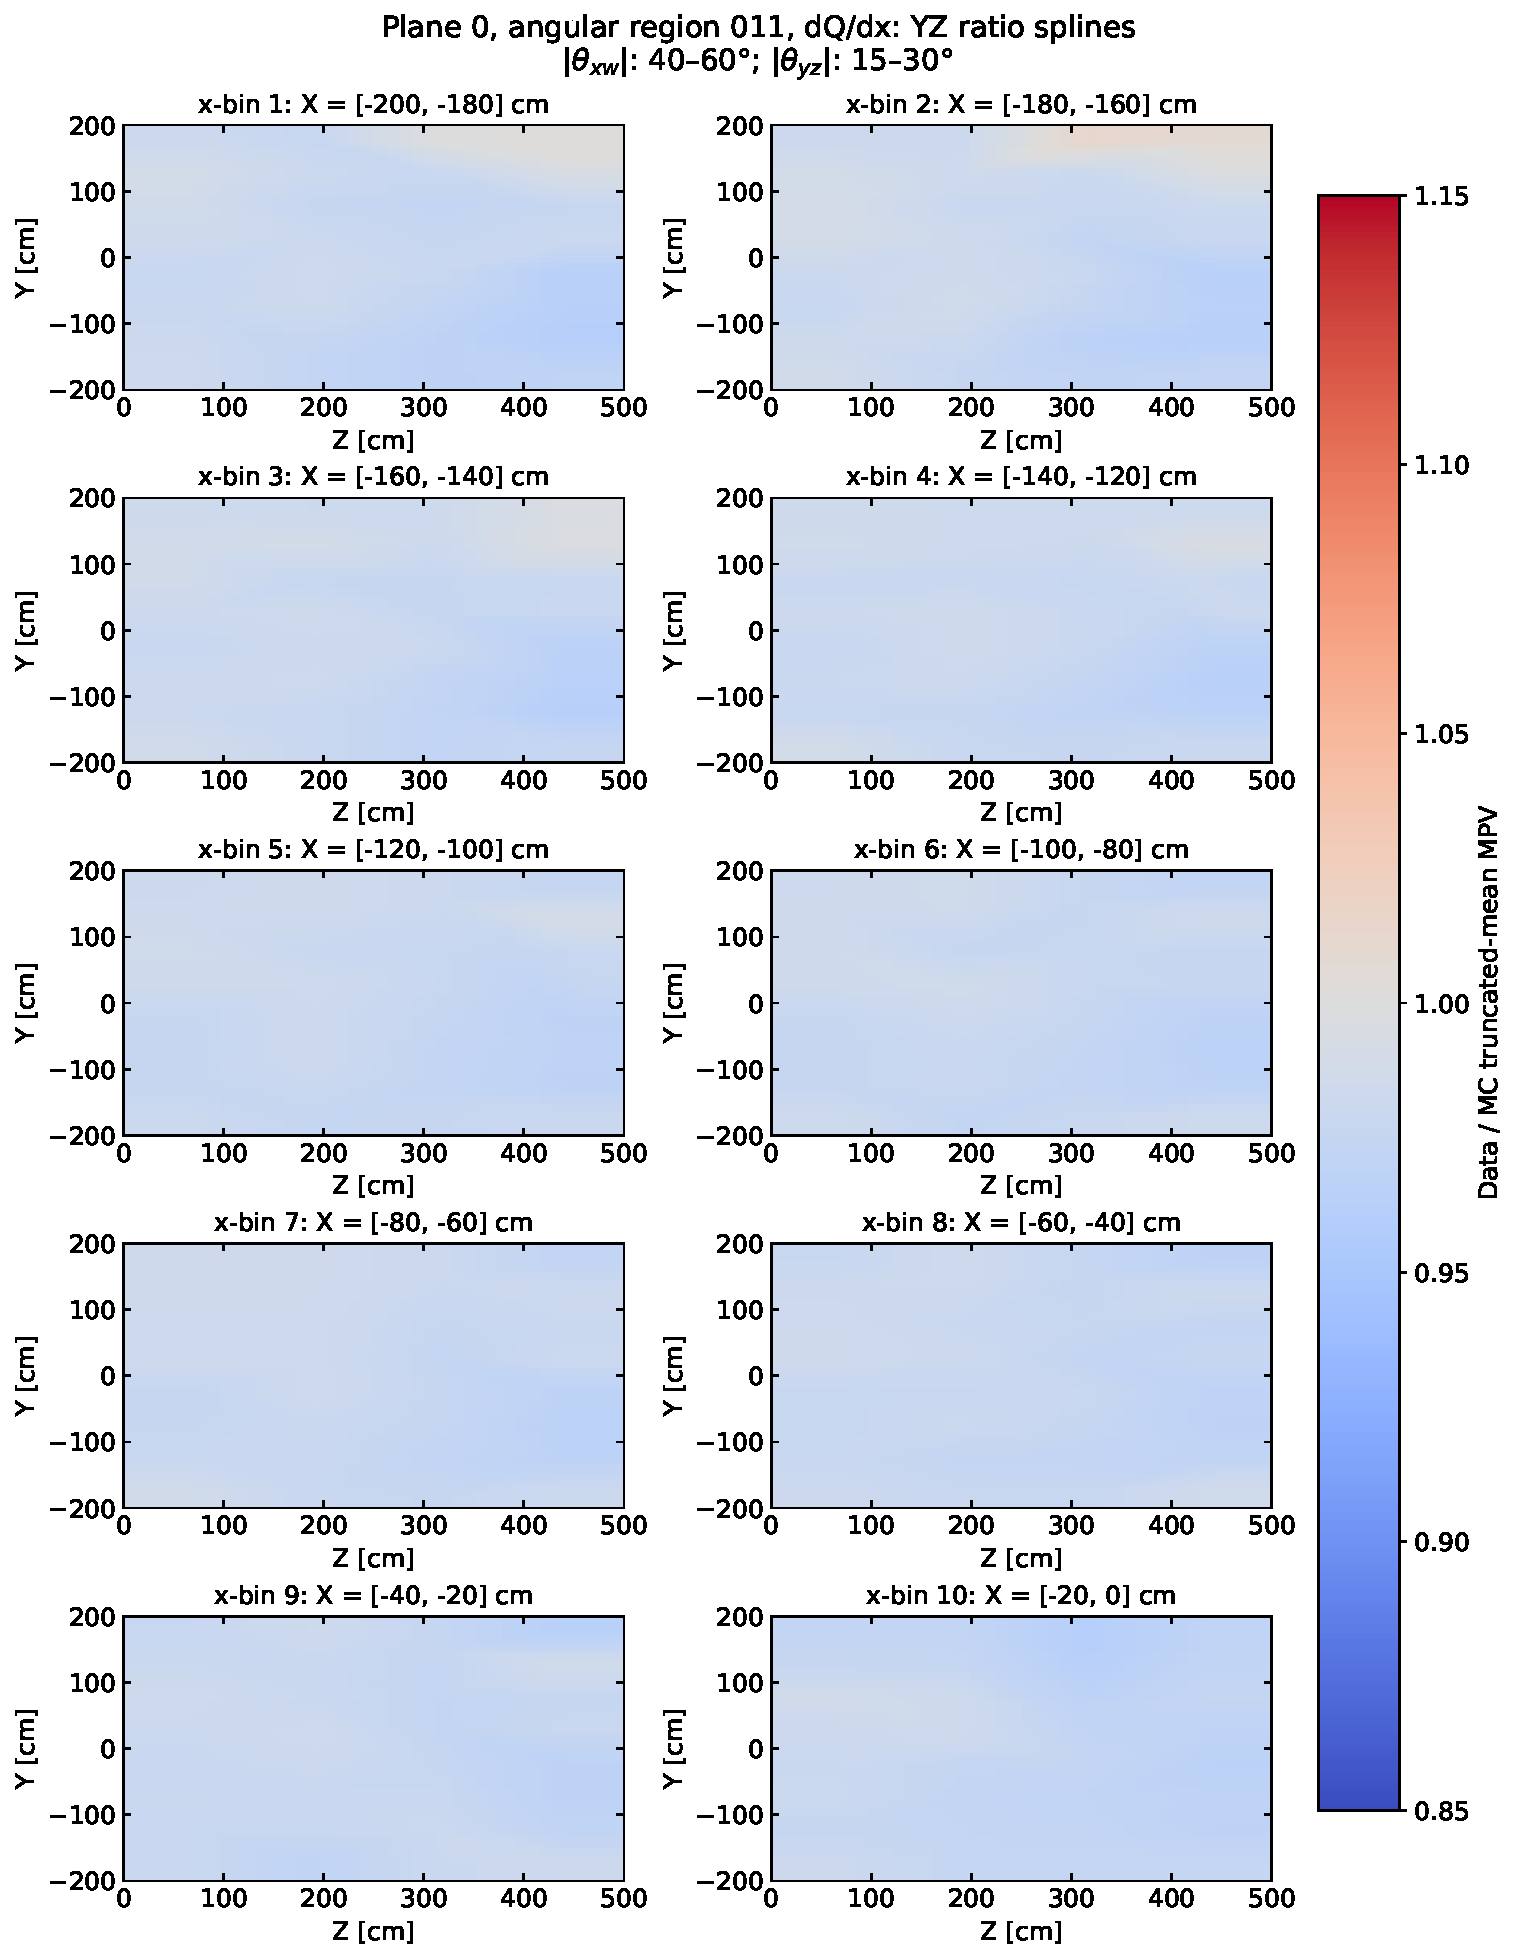
\includegraphics[width=\textwidth,height=0.80\textheight,keepaspectratio]{Figures/WireModXYZ/summary/plane0/anglebin_dq_plane0_region011_xyz_ratio_spline_summary_linear.pdf}
\caption{Plane 0, angular region 011: dQ/dx YZ data/MC ratio surfaces for all populated x-bins. The folded angular selection is $|\theta_{xw}|\in[40,60]^\circ$ and $|\theta_{yz}|\in[15,30]^\circ$.}
\label{fig:xyz_linear_dq_plane0_region011}
\end{figure}

\clearpage
\begin{figure}[H]
\centering
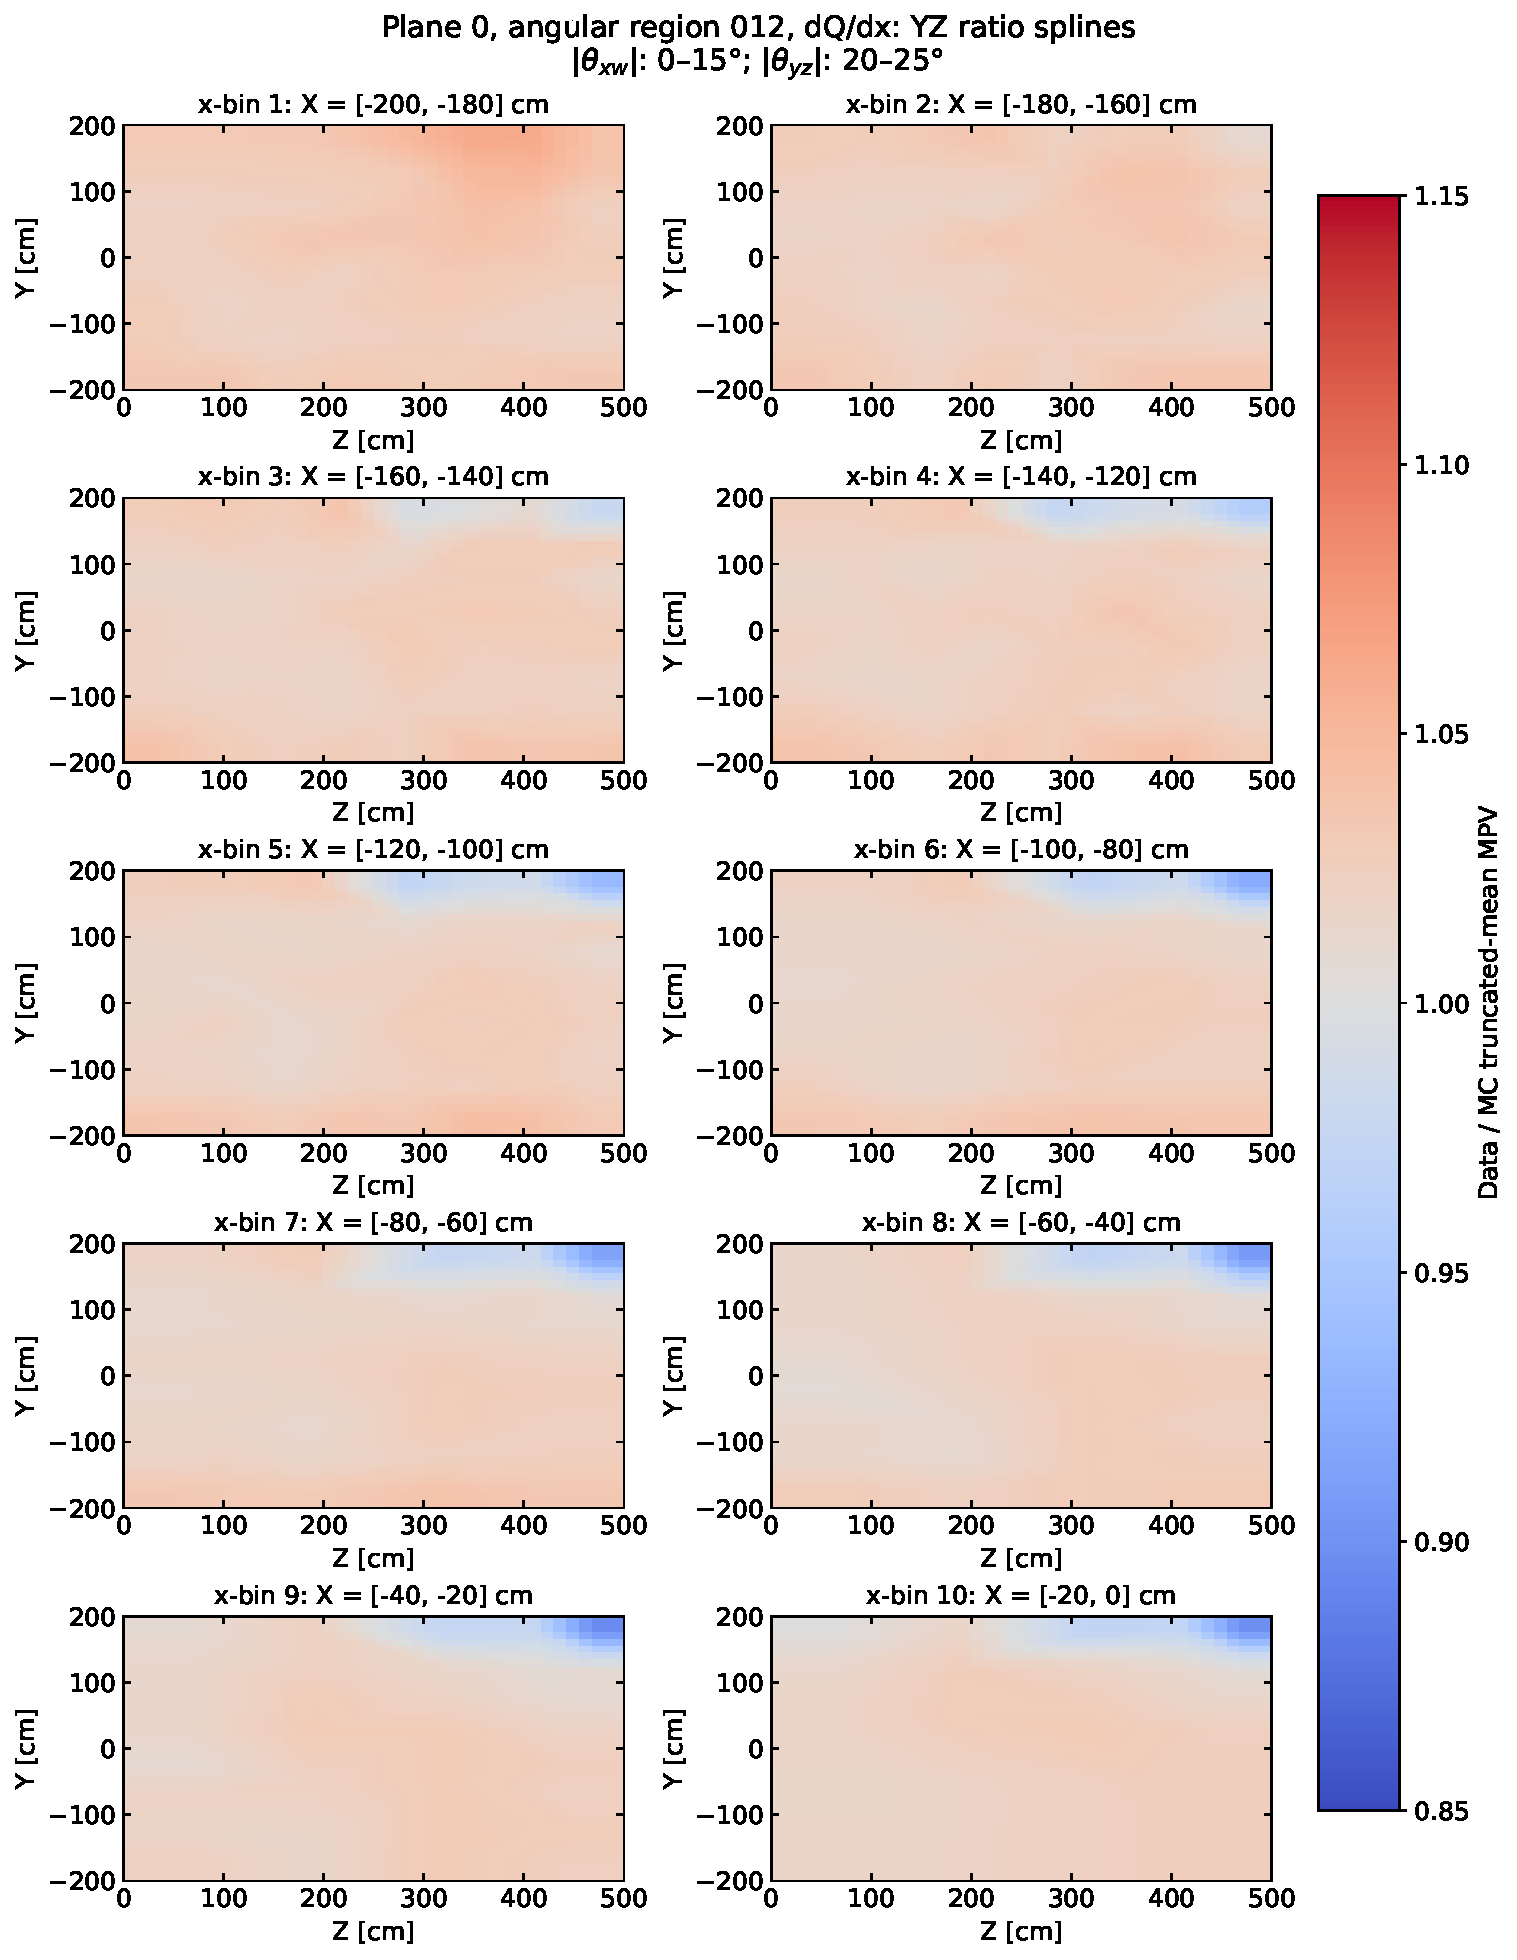
\includegraphics[width=\textwidth,height=0.80\textheight,keepaspectratio]{Figures/WireModXYZ/summary/plane0/anglebin_dq_plane0_region012_xyz_ratio_spline_summary_linear.pdf}
\caption{Plane 0, angular region 012: dQ/dx YZ data/MC ratio surfaces for all populated x-bins. The folded angular selection is $|\theta_{xw}|\in[0,15]^\circ$ and $|\theta_{yz}|\in[20,25]^\circ$.}
\label{fig:xyz_linear_dq_plane0_region012}
\end{figure}

\clearpage
\begin{figure}[H]
\centering
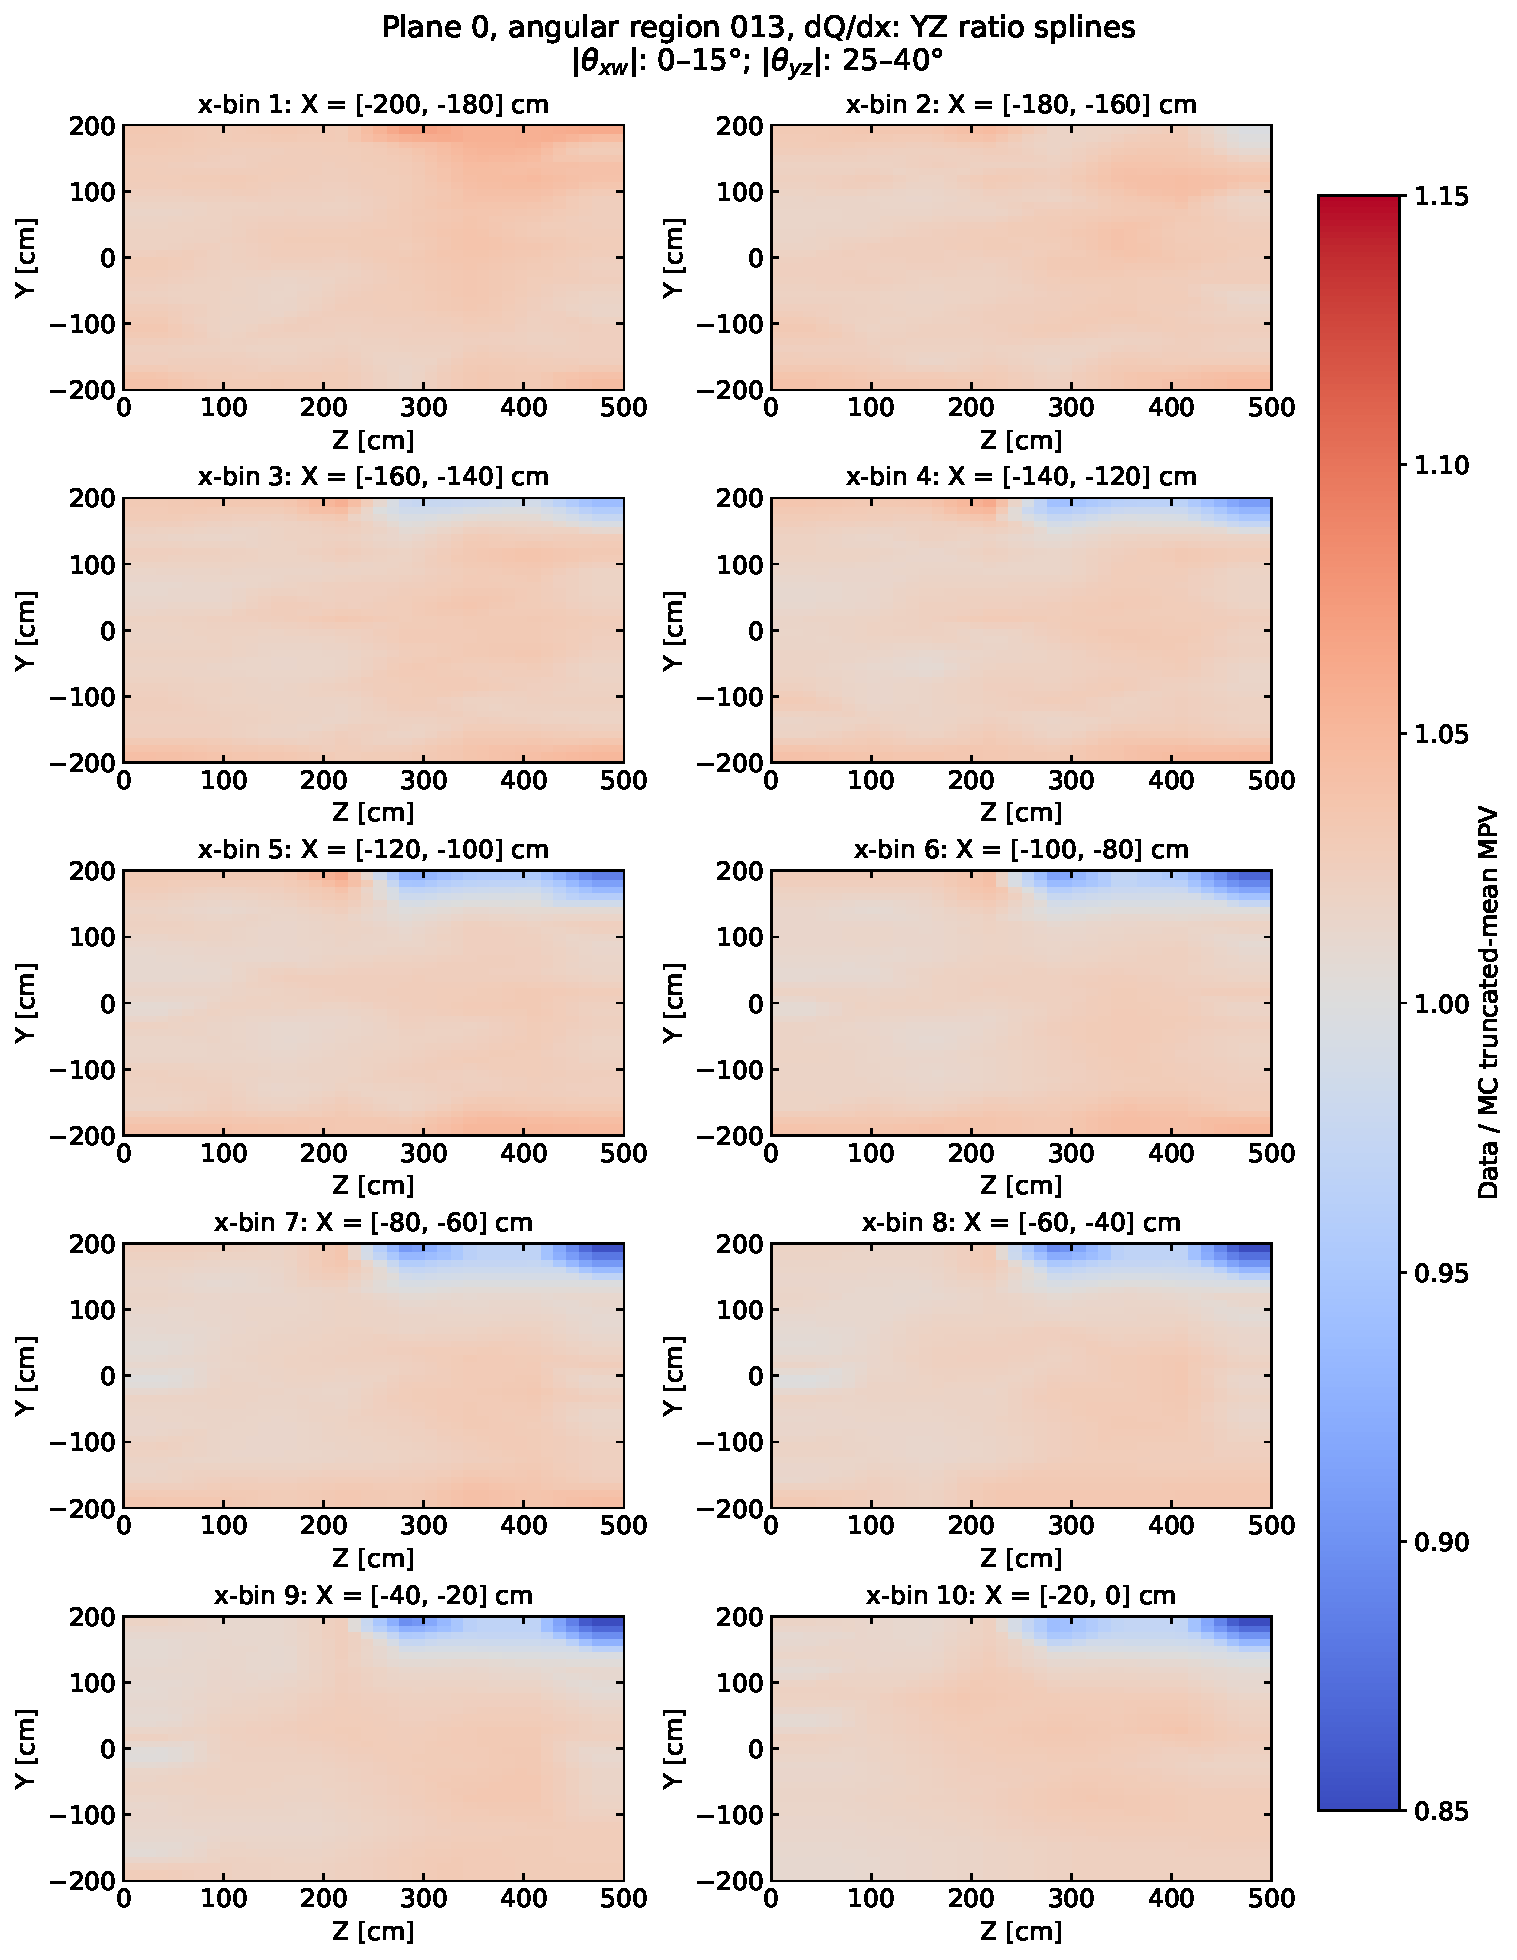
\includegraphics[width=\textwidth,height=0.80\textheight,keepaspectratio]{Figures/WireModXYZ/summary/plane0/anglebin_dq_plane0_region013_xyz_ratio_spline_summary_linear.pdf}
\caption{Plane 0, angular region 013: dQ/dx YZ data/MC ratio surfaces for all populated x-bins. The folded angular selection is $|\theta_{xw}|\in[0,15]^\circ$ and $|\theta_{yz}|\in[25,40]^\circ$.}
\label{fig:xyz_linear_dq_plane0_region013}
\end{figure}

\clearpage
\begin{figure}[H]
\centering
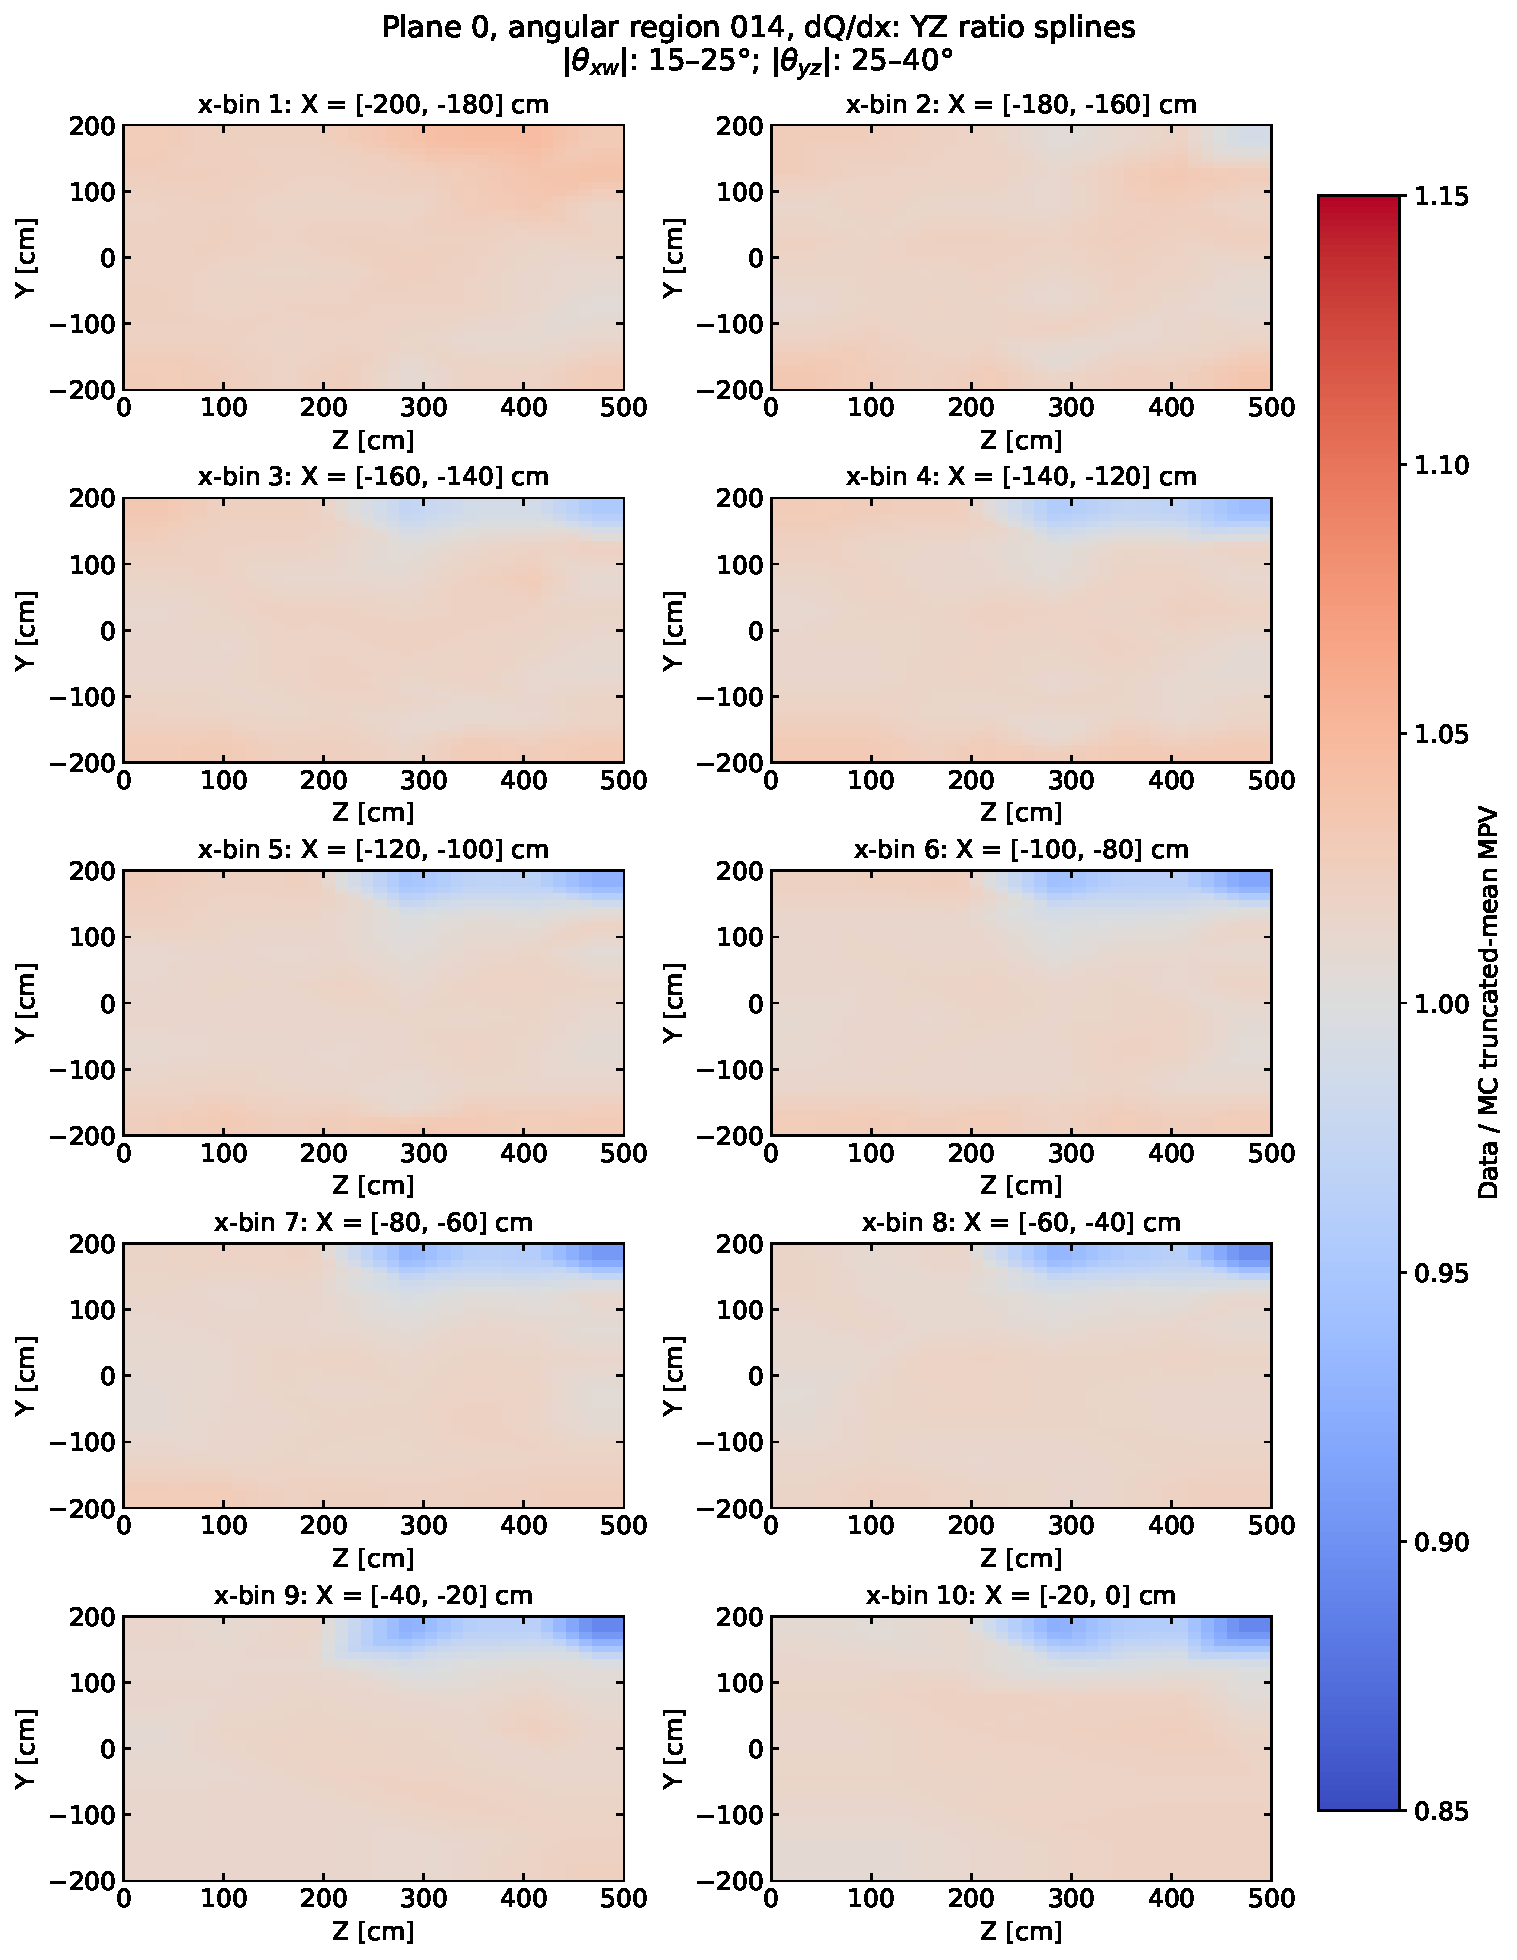
\includegraphics[width=\textwidth,height=0.80\textheight,keepaspectratio]{Figures/WireModXYZ/summary/plane0/anglebin_dq_plane0_region014_xyz_ratio_spline_summary_linear.pdf}
\caption{Plane 0, angular region 014: dQ/dx YZ data/MC ratio surfaces for all populated x-bins. The folded angular selection is $|\theta_{xw}|\in[15,25]^\circ$ and $|\theta_{yz}|\in[25,40]^\circ$.}
\label{fig:xyz_linear_dq_plane0_region014}
\end{figure}

\clearpage
\begin{figure}[H]
\centering
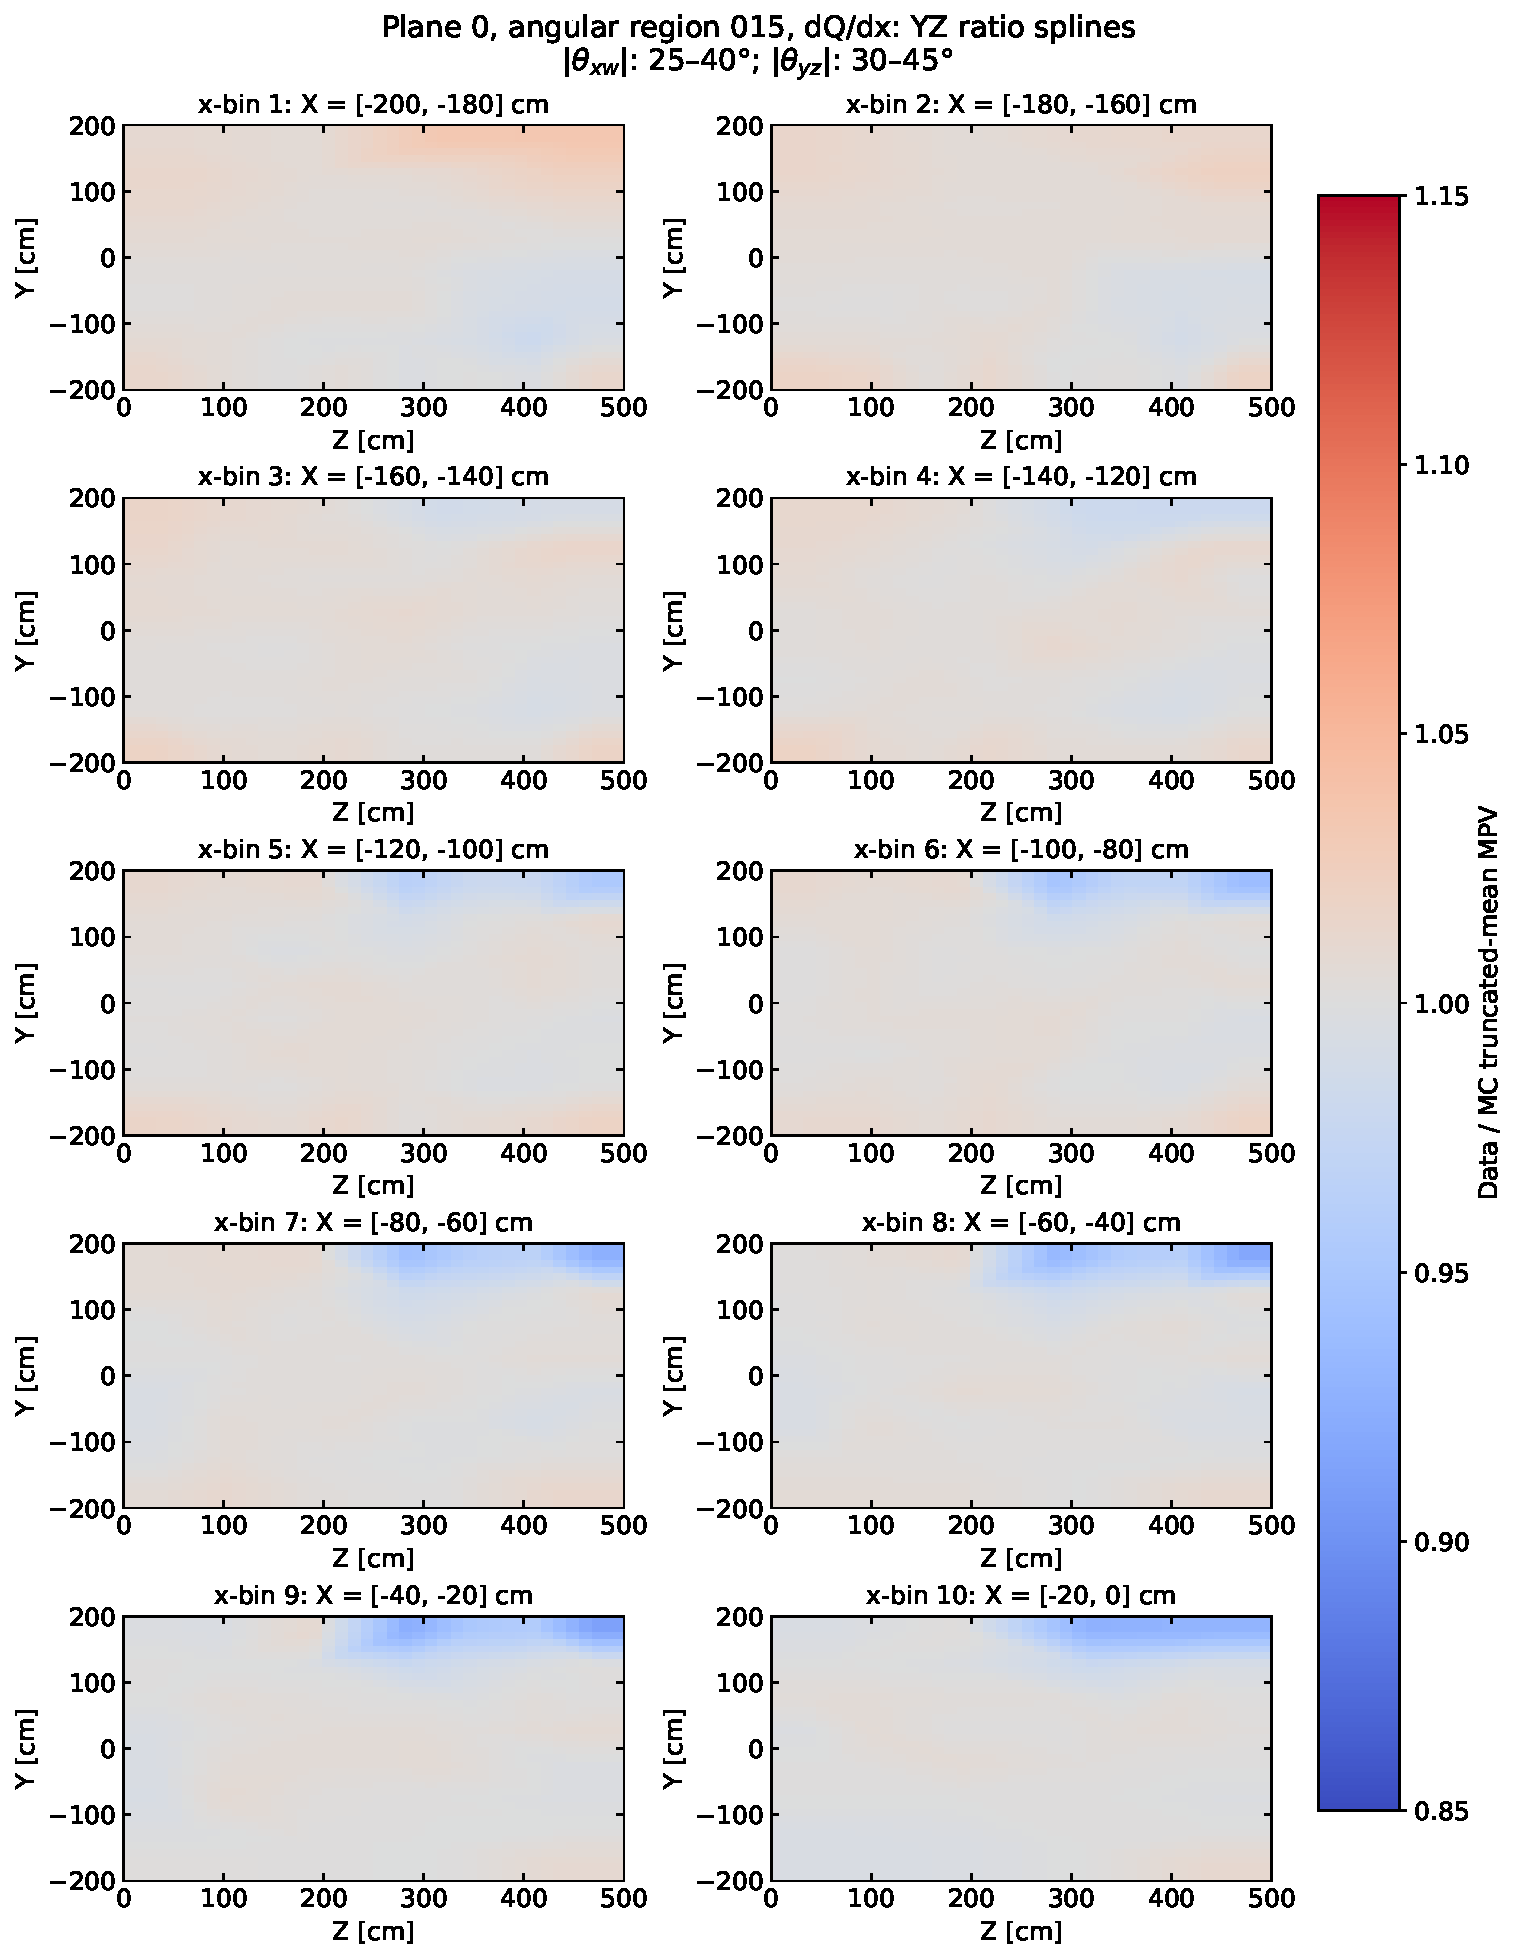
\includegraphics[width=\textwidth,height=0.80\textheight,keepaspectratio]{Figures/WireModXYZ/summary/plane0/anglebin_dq_plane0_region015_xyz_ratio_spline_summary_linear.pdf}
\caption{Plane 0, angular region 015: dQ/dx YZ data/MC ratio surfaces for all populated x-bins. The folded angular selection is $|\theta_{xw}|\in[25,40]^\circ$ and $|\theta_{yz}|\in[30,45]^\circ$.}
\label{fig:xyz_linear_dq_plane0_region015}
\end{figure}

\clearpage
\begin{figure}[H]
\centering
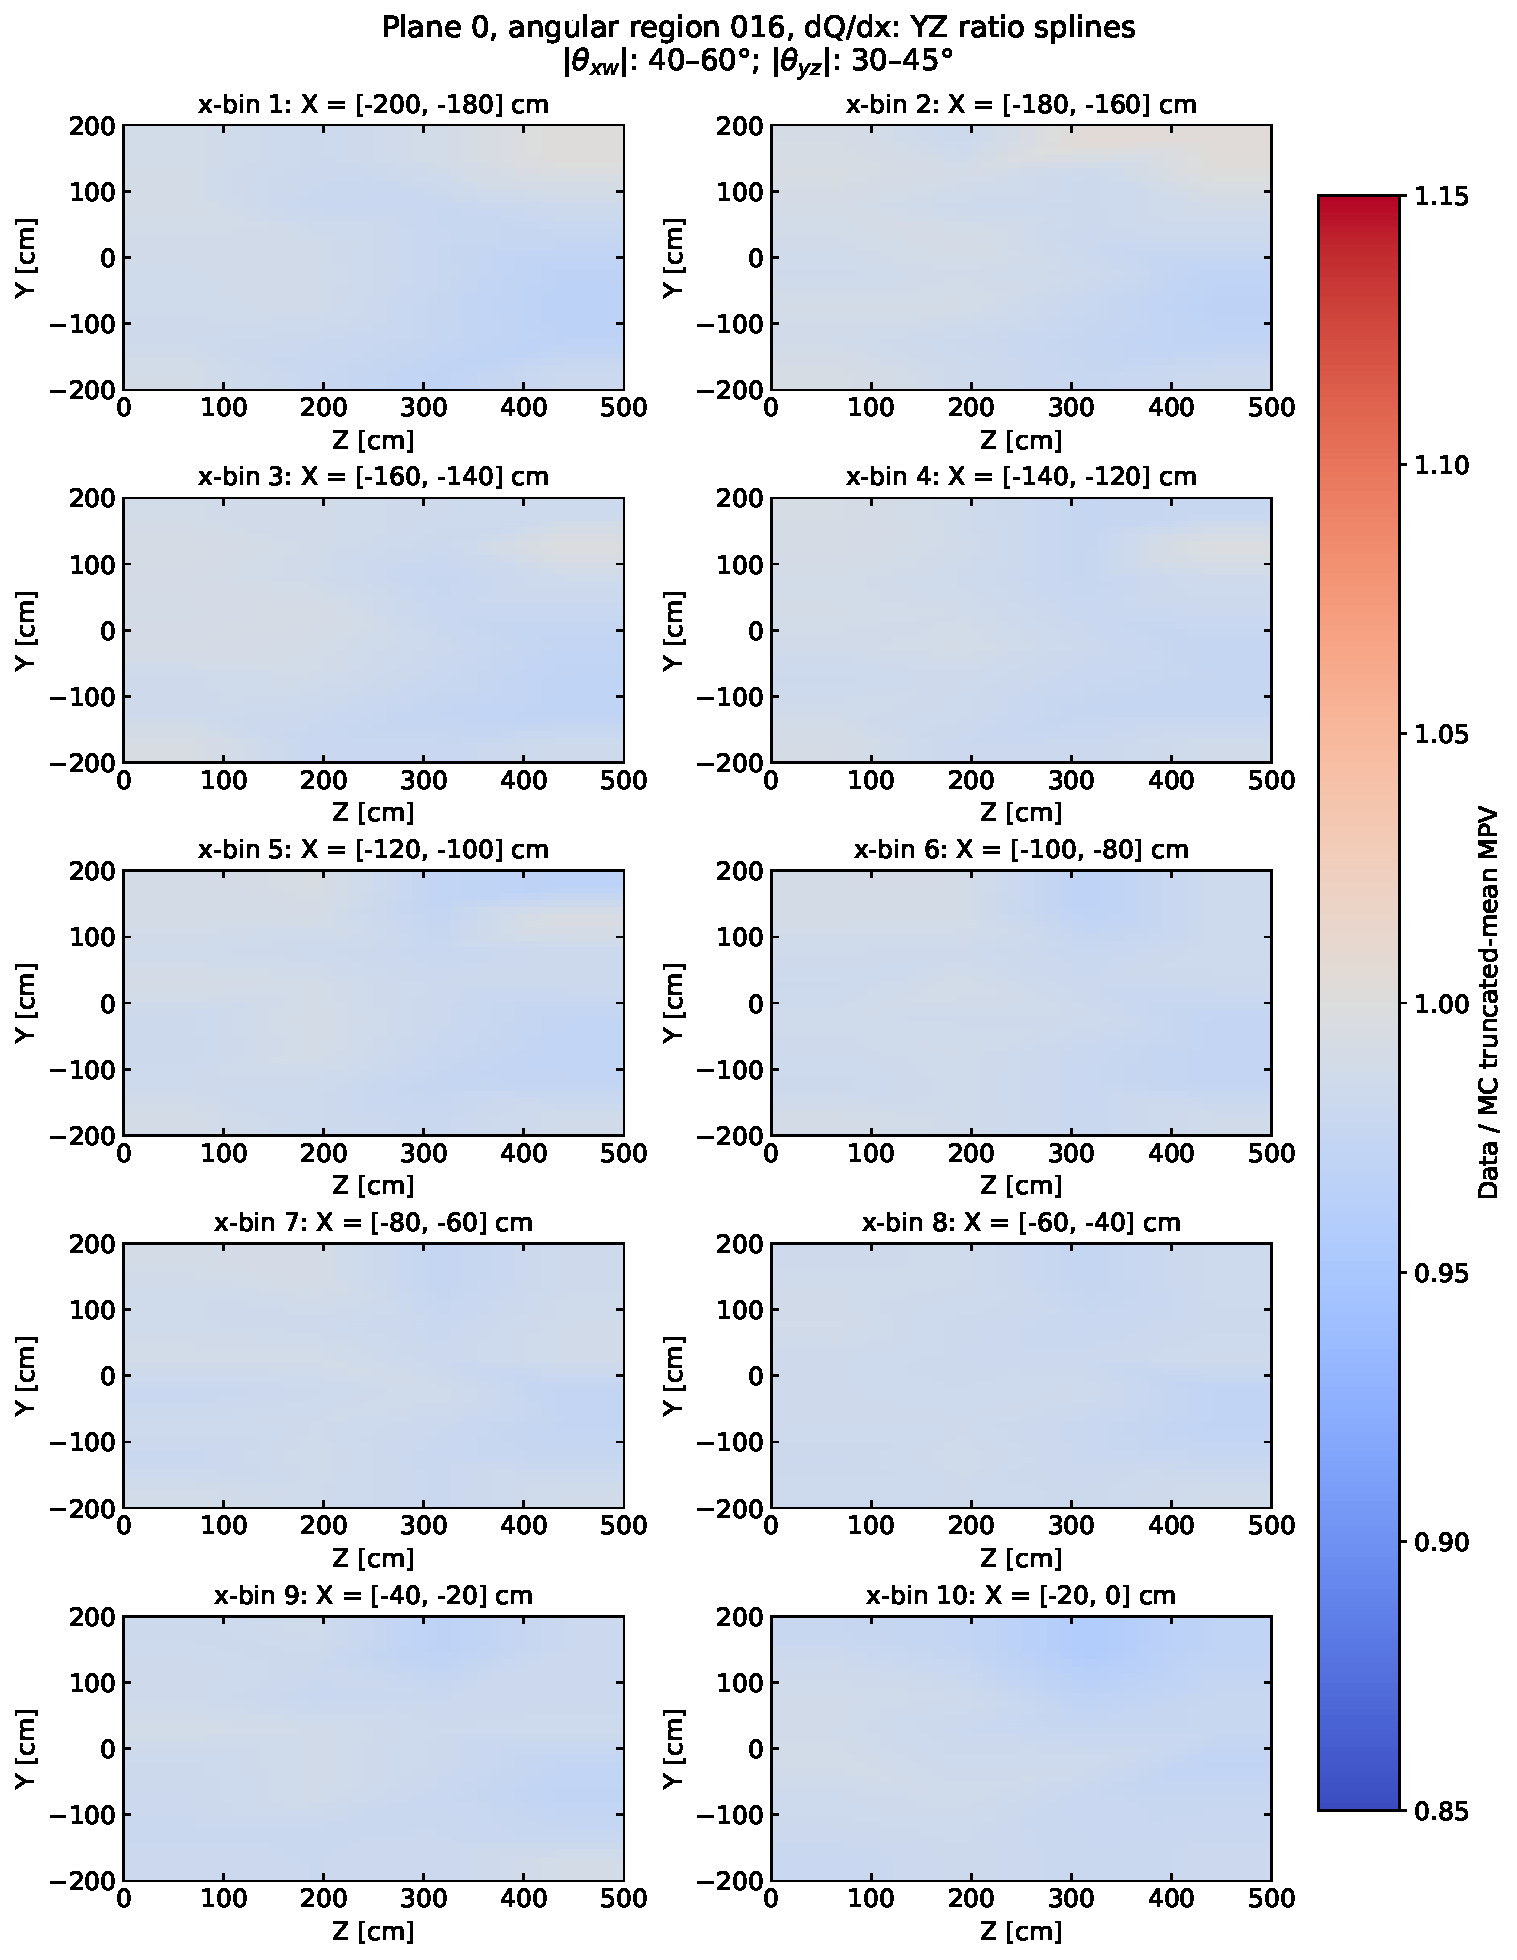
\includegraphics[width=\textwidth,height=0.80\textheight,keepaspectratio]{Figures/WireModXYZ/summary/plane0/anglebin_dq_plane0_region016_xyz_ratio_spline_summary_linear.pdf}
\caption{Plane 0, angular region 016: dQ/dx YZ data/MC ratio surfaces for all populated x-bins. The folded angular selection is $|\theta_{xw}|\in[40,60]^\circ$ and $|\theta_{yz}|\in[30,45]^\circ$.}
\label{fig:xyz_linear_dq_plane0_region016}
\end{figure}

\clearpage
\begin{figure}[H]
\centering
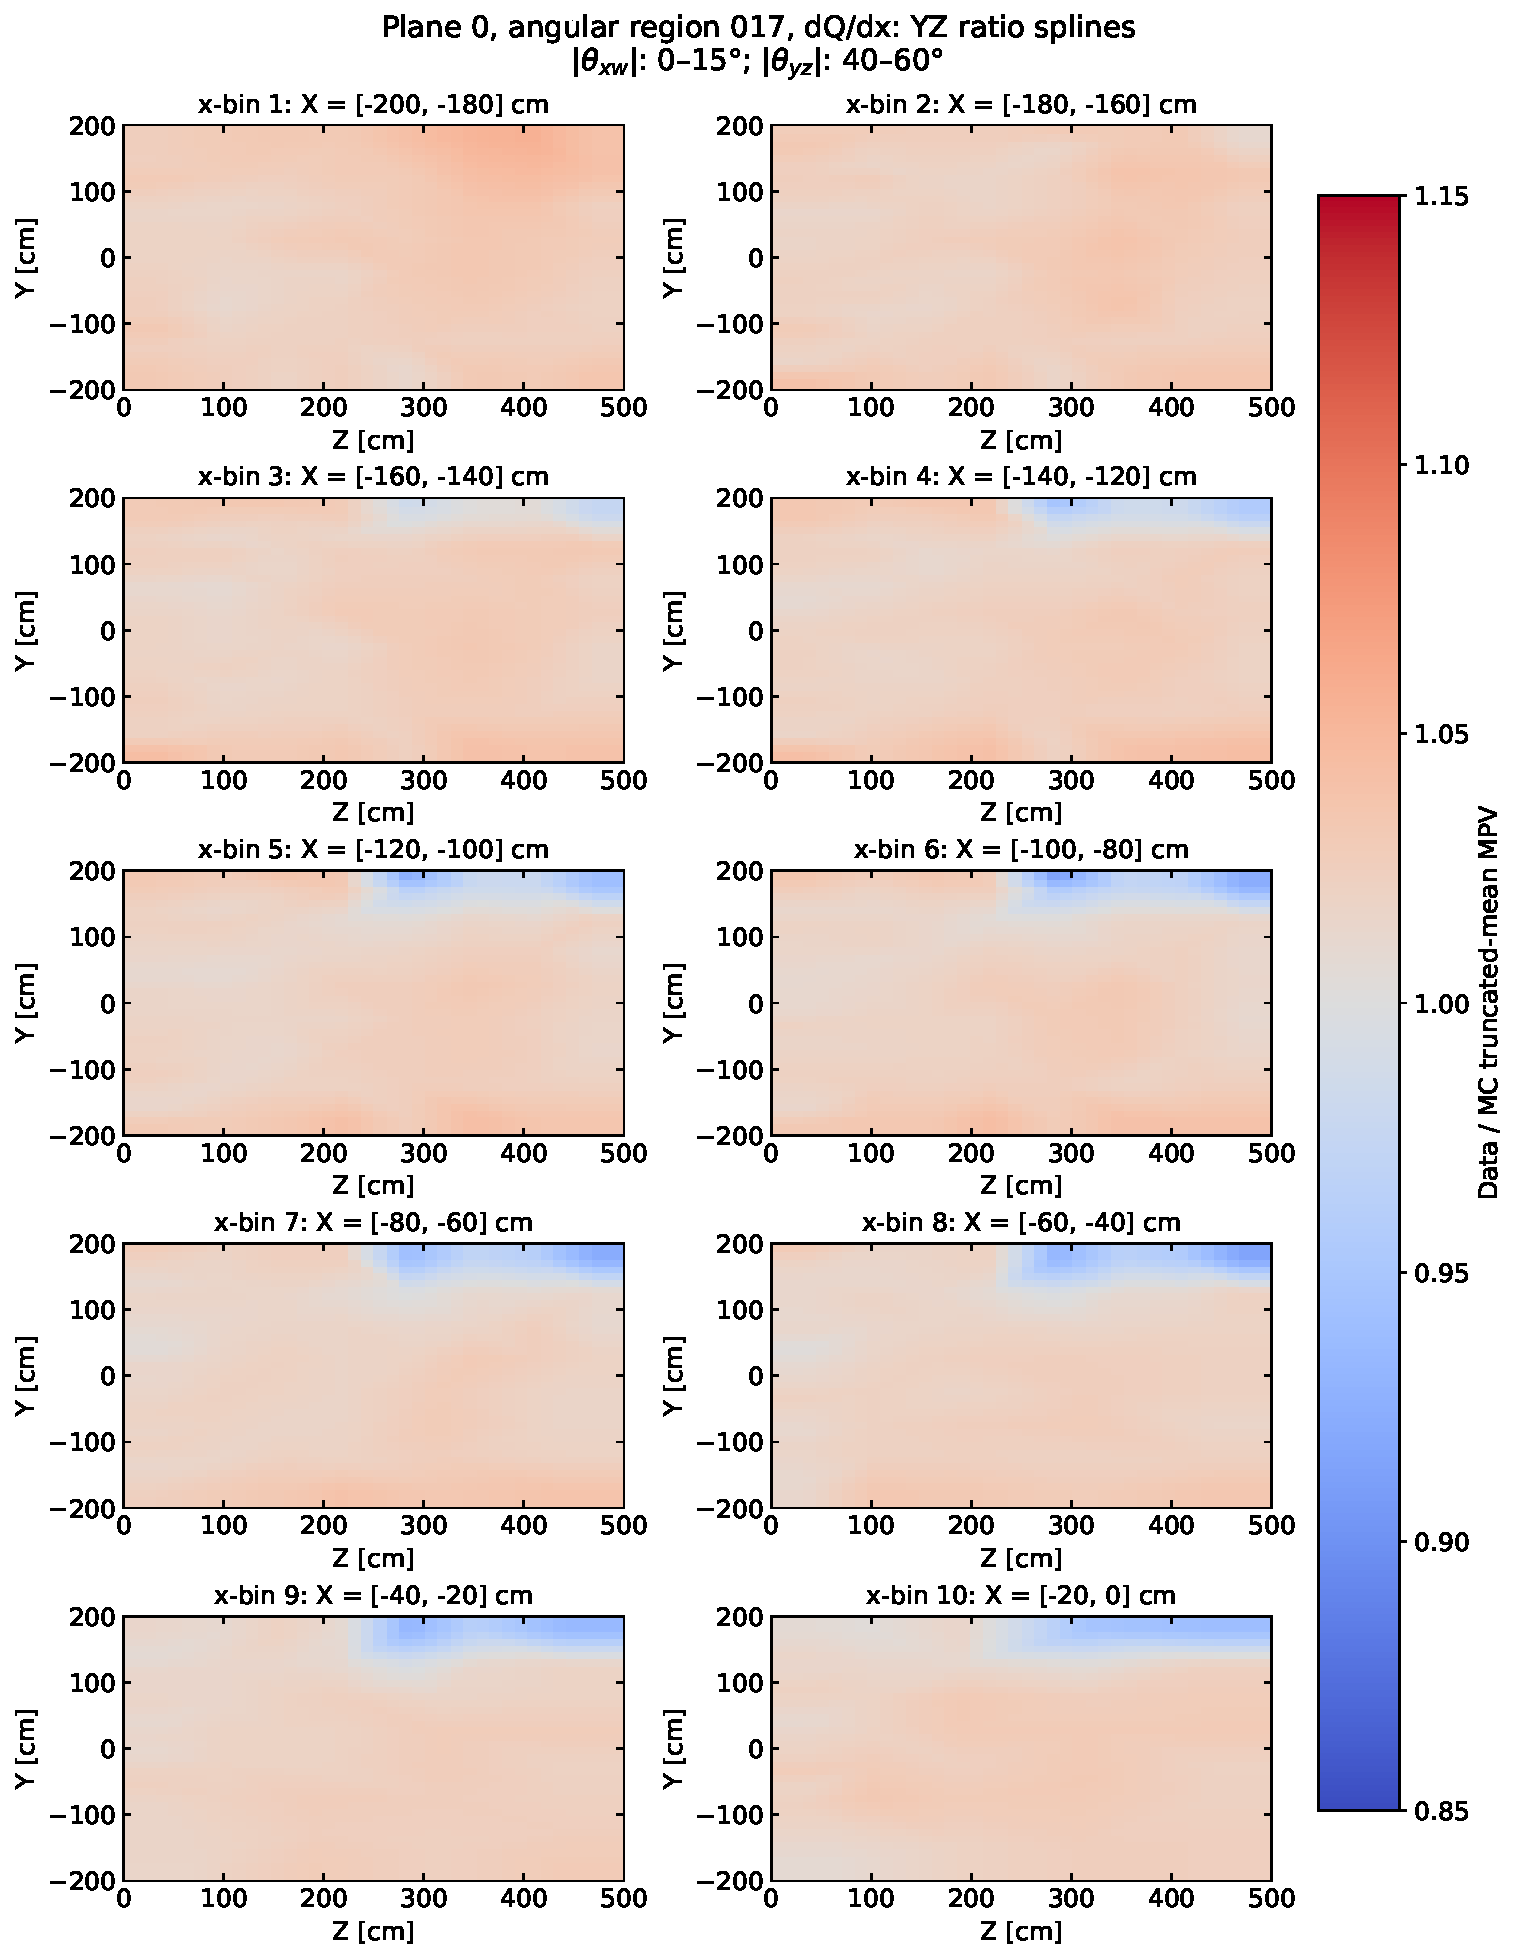
\includegraphics[width=\textwidth,height=0.80\textheight,keepaspectratio]{Figures/WireModXYZ/summary/plane0/anglebin_dq_plane0_region017_xyz_ratio_spline_summary_linear.pdf}
\caption{Plane 0, angular region 017: dQ/dx YZ data/MC ratio surfaces for all populated x-bins. The folded angular selection is $|\theta_{xw}|\in[0,15]^\circ$ and $|\theta_{yz}|\in[40,60]^\circ$.}
\label{fig:xyz_linear_dq_plane0_region017}
\end{figure}

\clearpage
\begin{figure}[H]
\centering
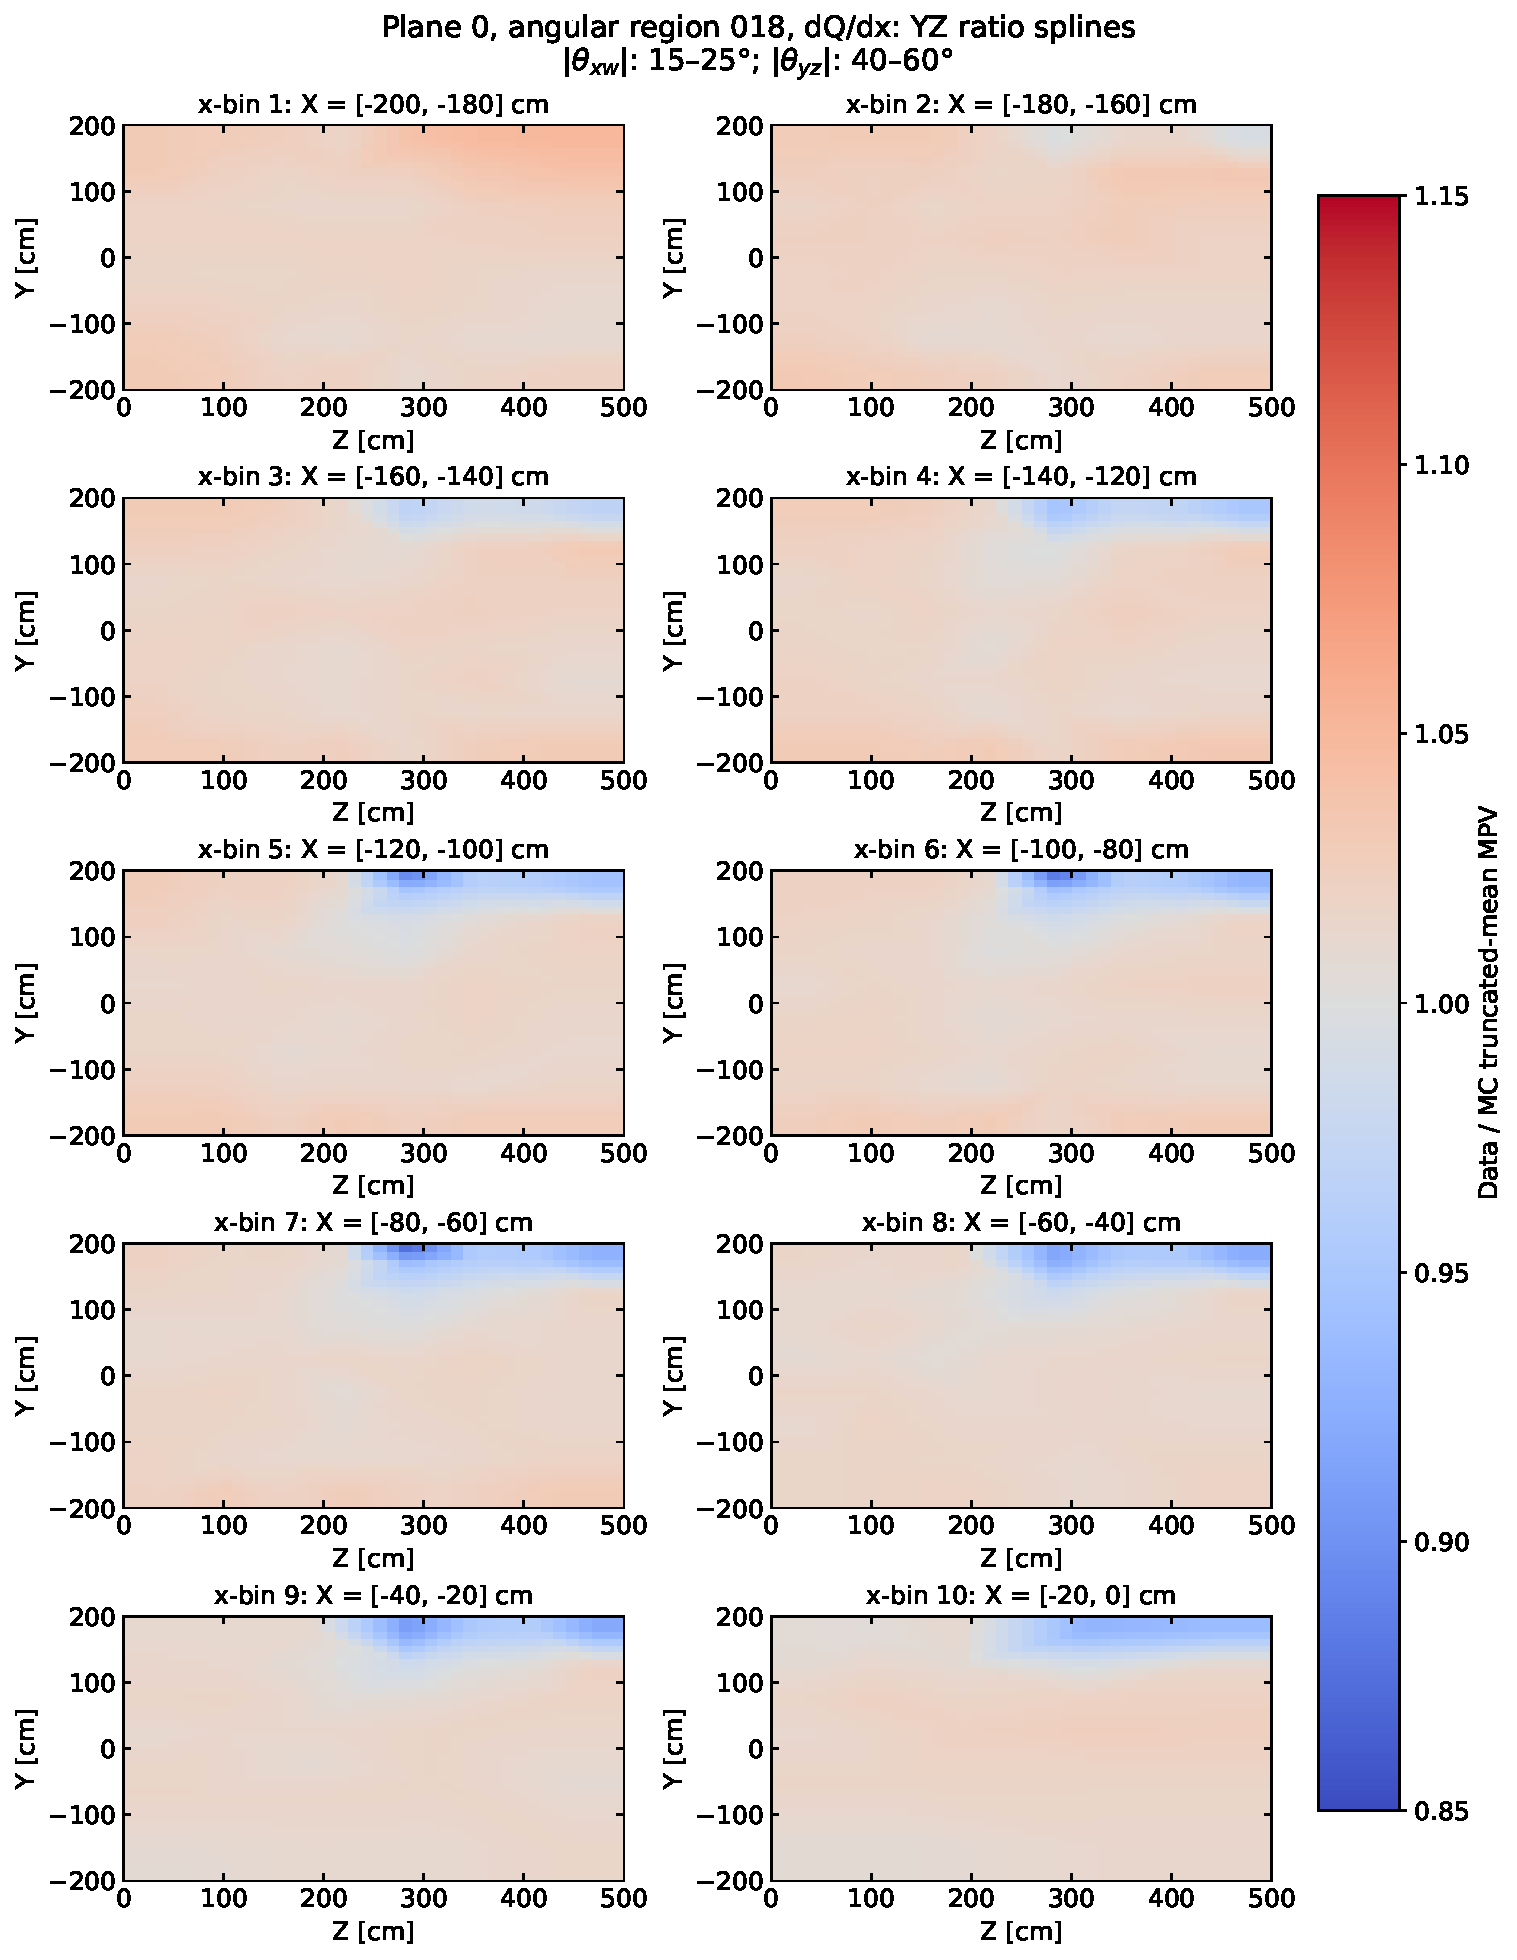
\includegraphics[width=\textwidth,height=0.80\textheight,keepaspectratio]{Figures/WireModXYZ/summary/plane0/anglebin_dq_plane0_region018_xyz_ratio_spline_summary_linear.pdf}
\caption{Plane 0, angular region 018: dQ/dx YZ data/MC ratio surfaces for all populated x-bins. The folded angular selection is $|\theta_{xw}|\in[15,25]^\circ$ and $|\theta_{yz}|\in[40,60]^\circ$.}
\label{fig:xyz_linear_dq_plane0_region018}
\end{figure}

\clearpage
\begin{figure}[H]
\centering
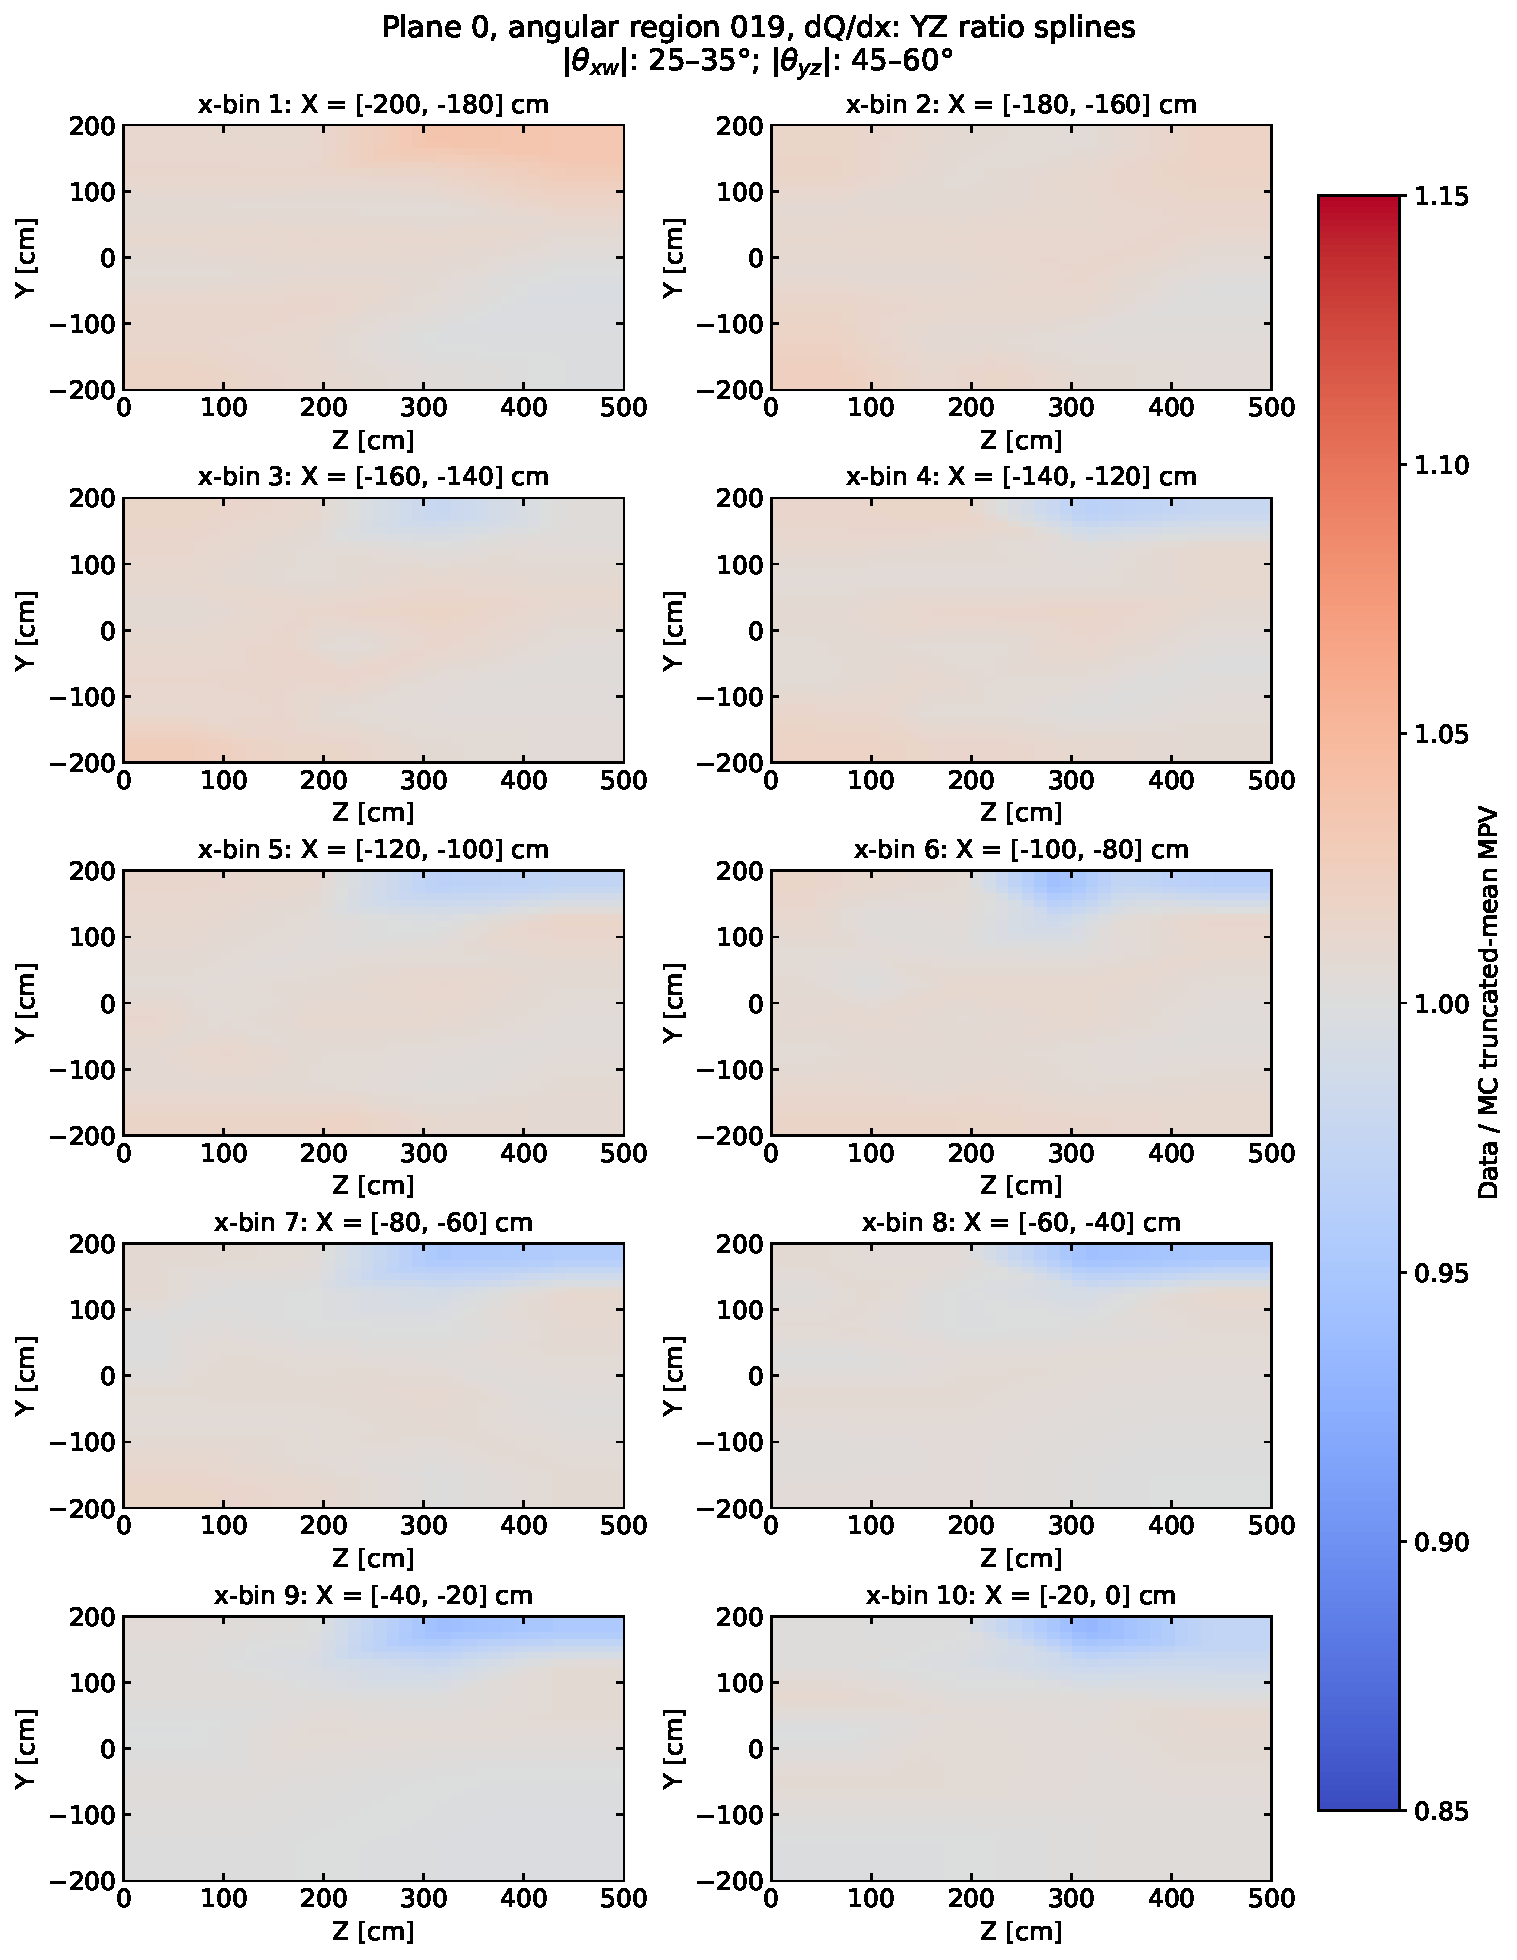
\includegraphics[width=\textwidth,height=0.80\textheight,keepaspectratio]{Figures/WireModXYZ/summary/plane0/anglebin_dq_plane0_region019_xyz_ratio_spline_summary_linear.pdf}
\caption{Plane 0, angular region 019: dQ/dx YZ data/MC ratio surfaces for all populated x-bins. The folded angular selection is $|\theta_{xw}|\in[25,35]^\circ$ and $|\theta_{yz}|\in[45,60]^\circ$.}
\label{fig:xyz_linear_dq_plane0_region019}
\end{figure}

\clearpage
\begin{figure}[H]
\centering
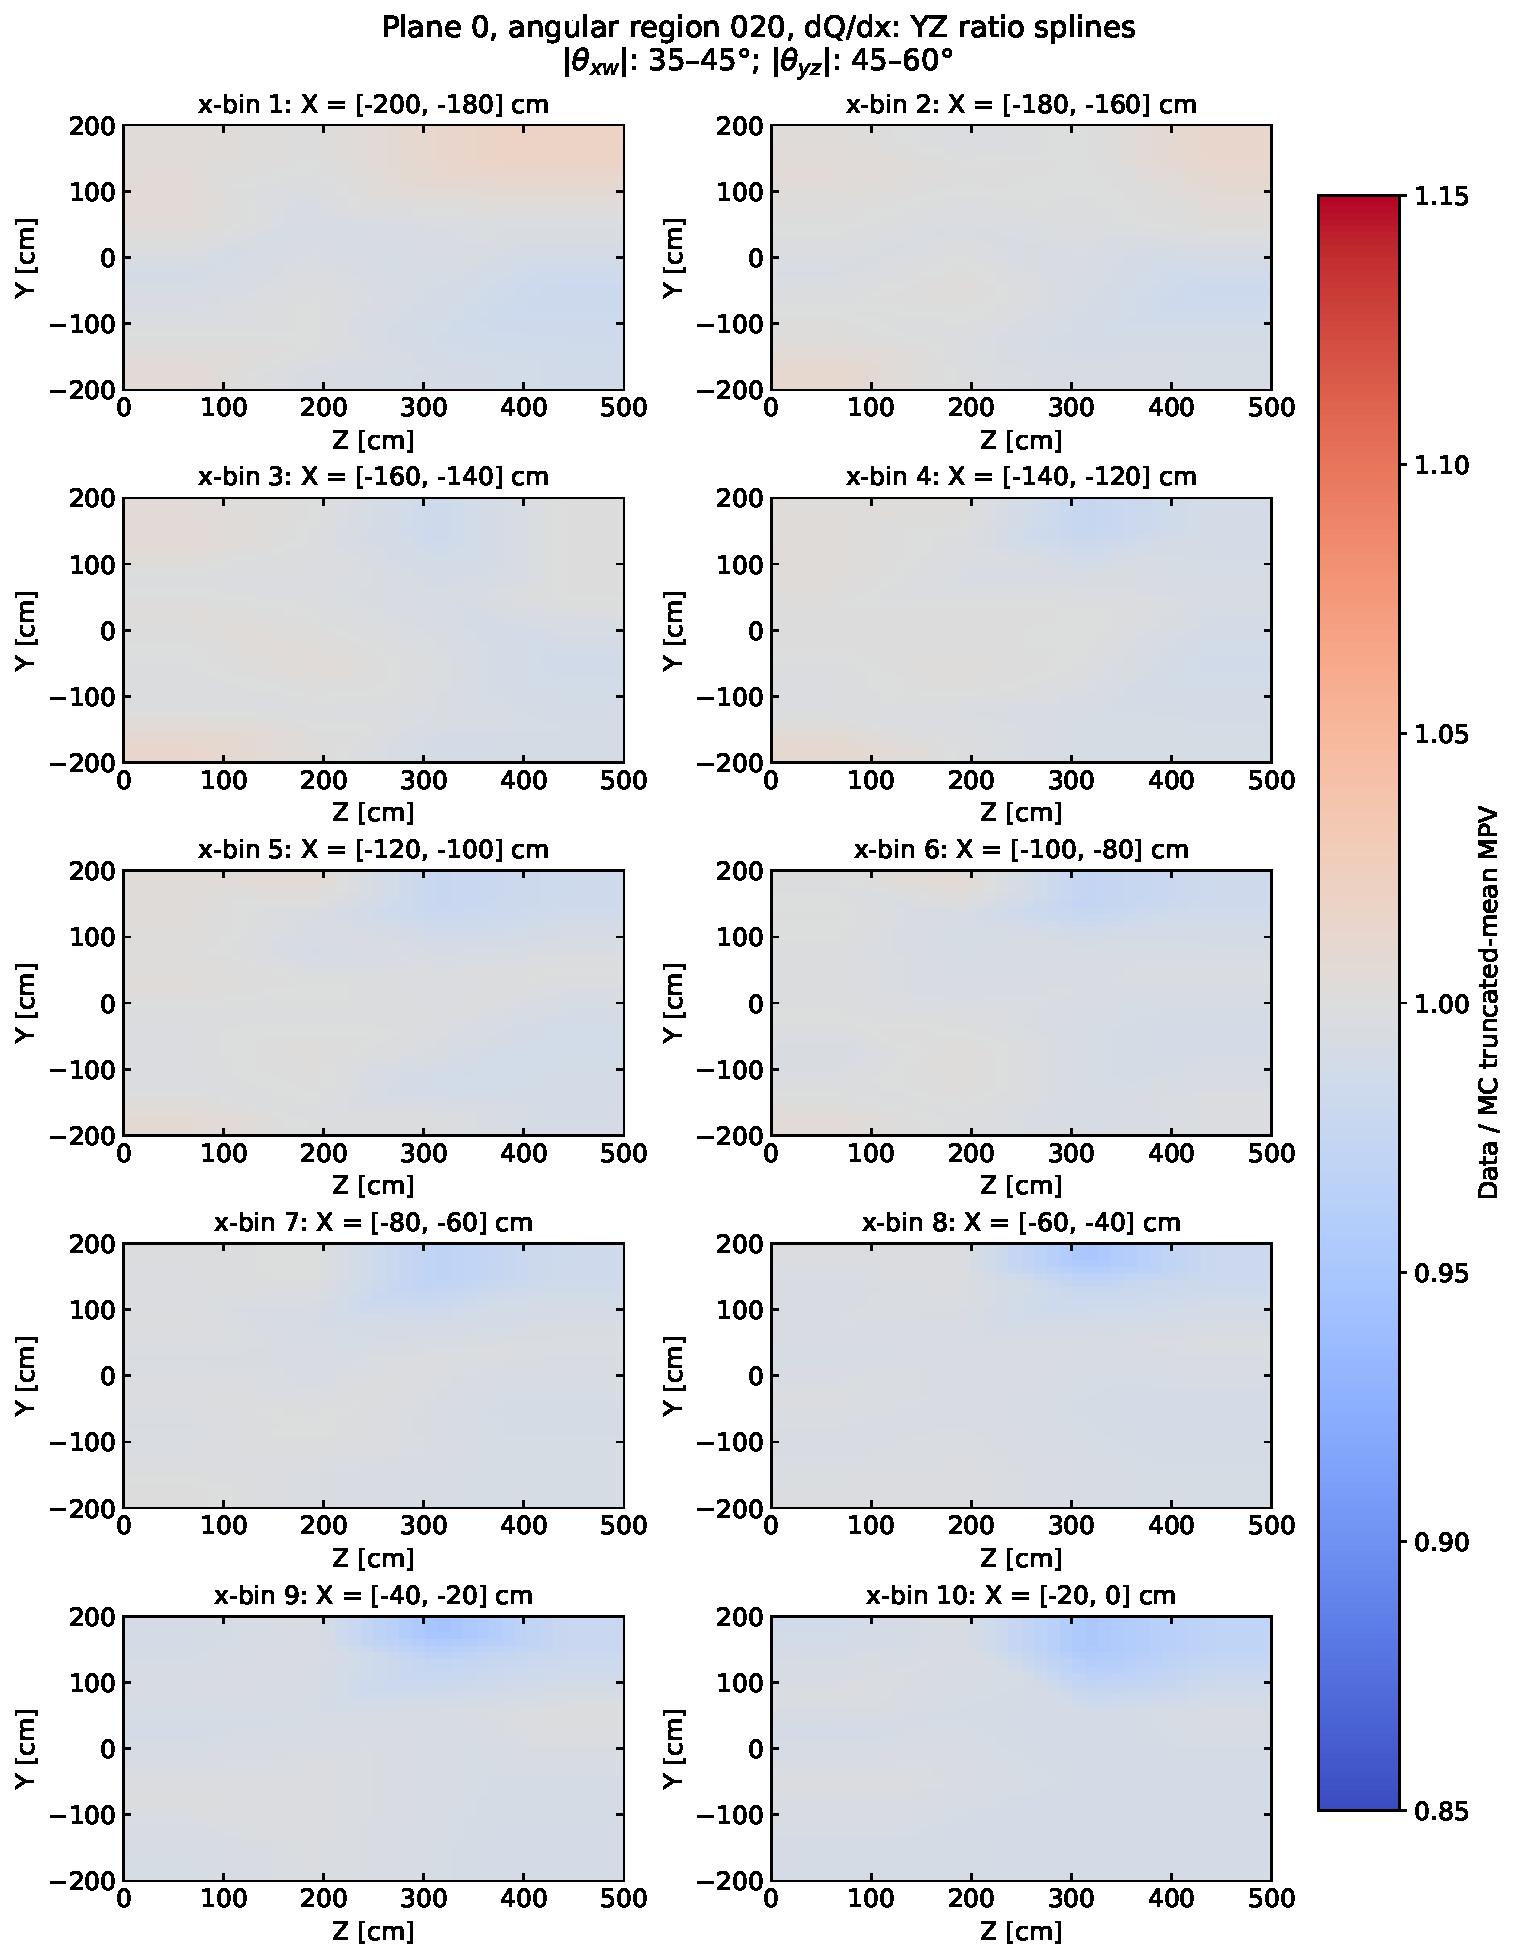
\includegraphics[width=\textwidth,height=0.80\textheight,keepaspectratio]{Figures/WireModXYZ/summary/plane0/anglebin_dq_plane0_region020_xyz_ratio_spline_summary_linear.pdf}
\caption{Plane 0, angular region 020: dQ/dx YZ data/MC ratio surfaces for all populated x-bins. The folded angular selection is $|\theta_{xw}|\in[35,45]^\circ$ and $|\theta_{yz}|\in[45,60]^\circ$.}
\label{fig:xyz_linear_dq_plane0_region020}
\end{figure}

\clearpage
\begin{figure}[H]
\centering
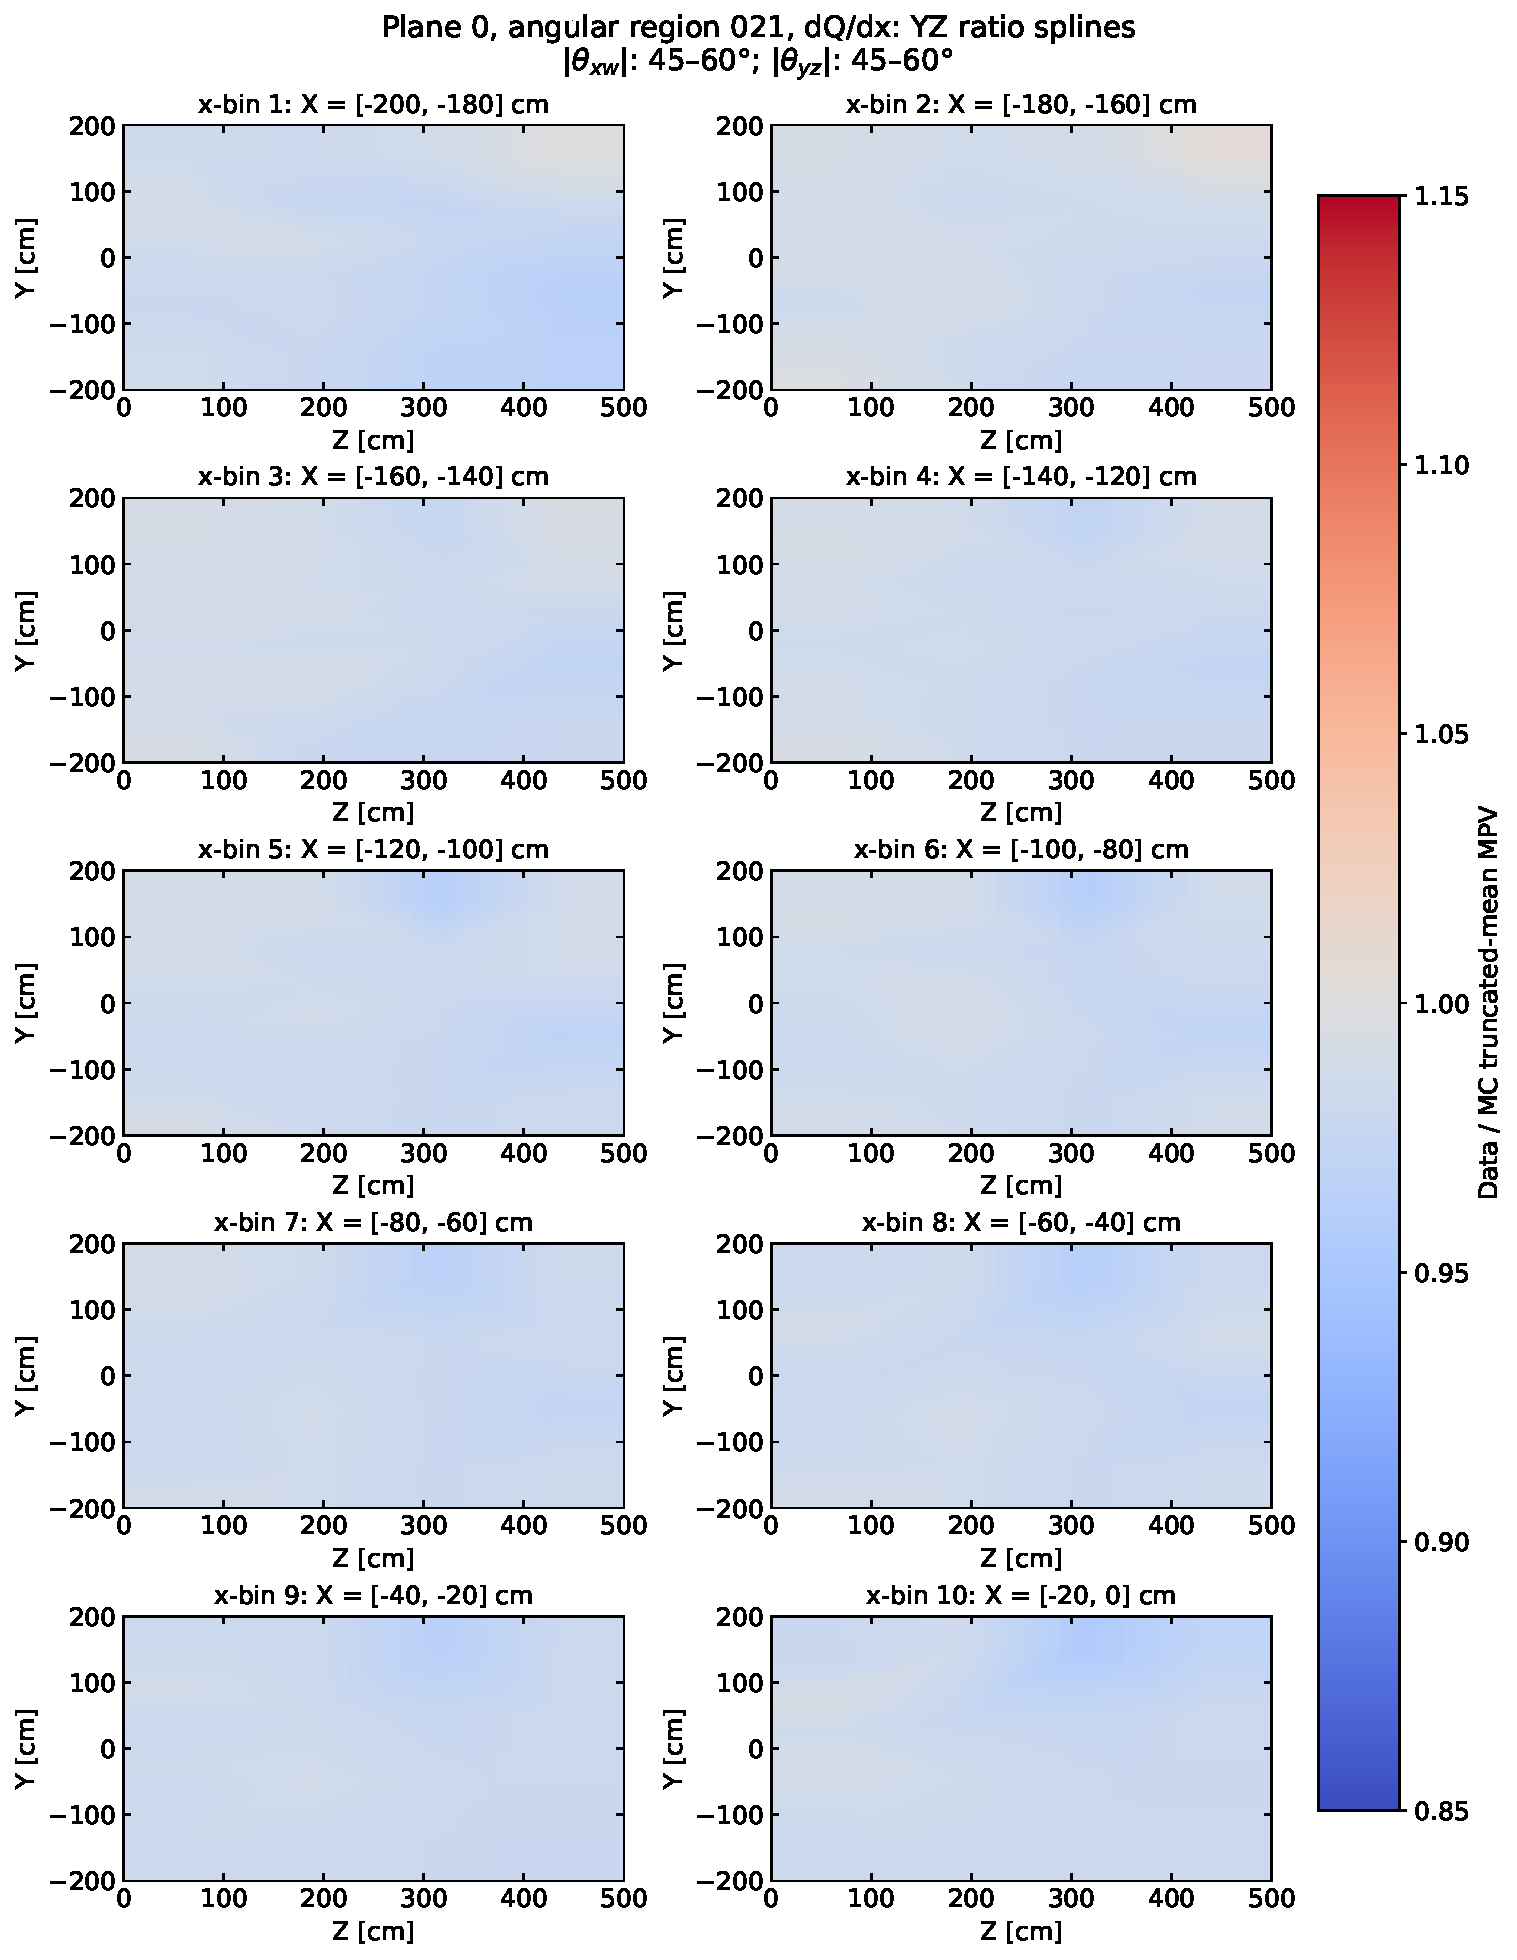
\includegraphics[width=\textwidth,height=0.80\textheight,keepaspectratio]{Figures/WireModXYZ/summary/plane0/anglebin_dq_plane0_region021_xyz_ratio_spline_summary_linear.pdf}
\caption{Plane 0, angular region 021: dQ/dx YZ data/MC ratio surfaces for all populated x-bins. The folded angular selection is $|\theta_{xw}|\in[45,60]^\circ$ and $|\theta_{yz}|\in[45,60]^\circ$.}
\label{fig:xyz_linear_dq_plane0_region021}
\end{figure}

\clearpage
\begin{figure}[H]
\centering
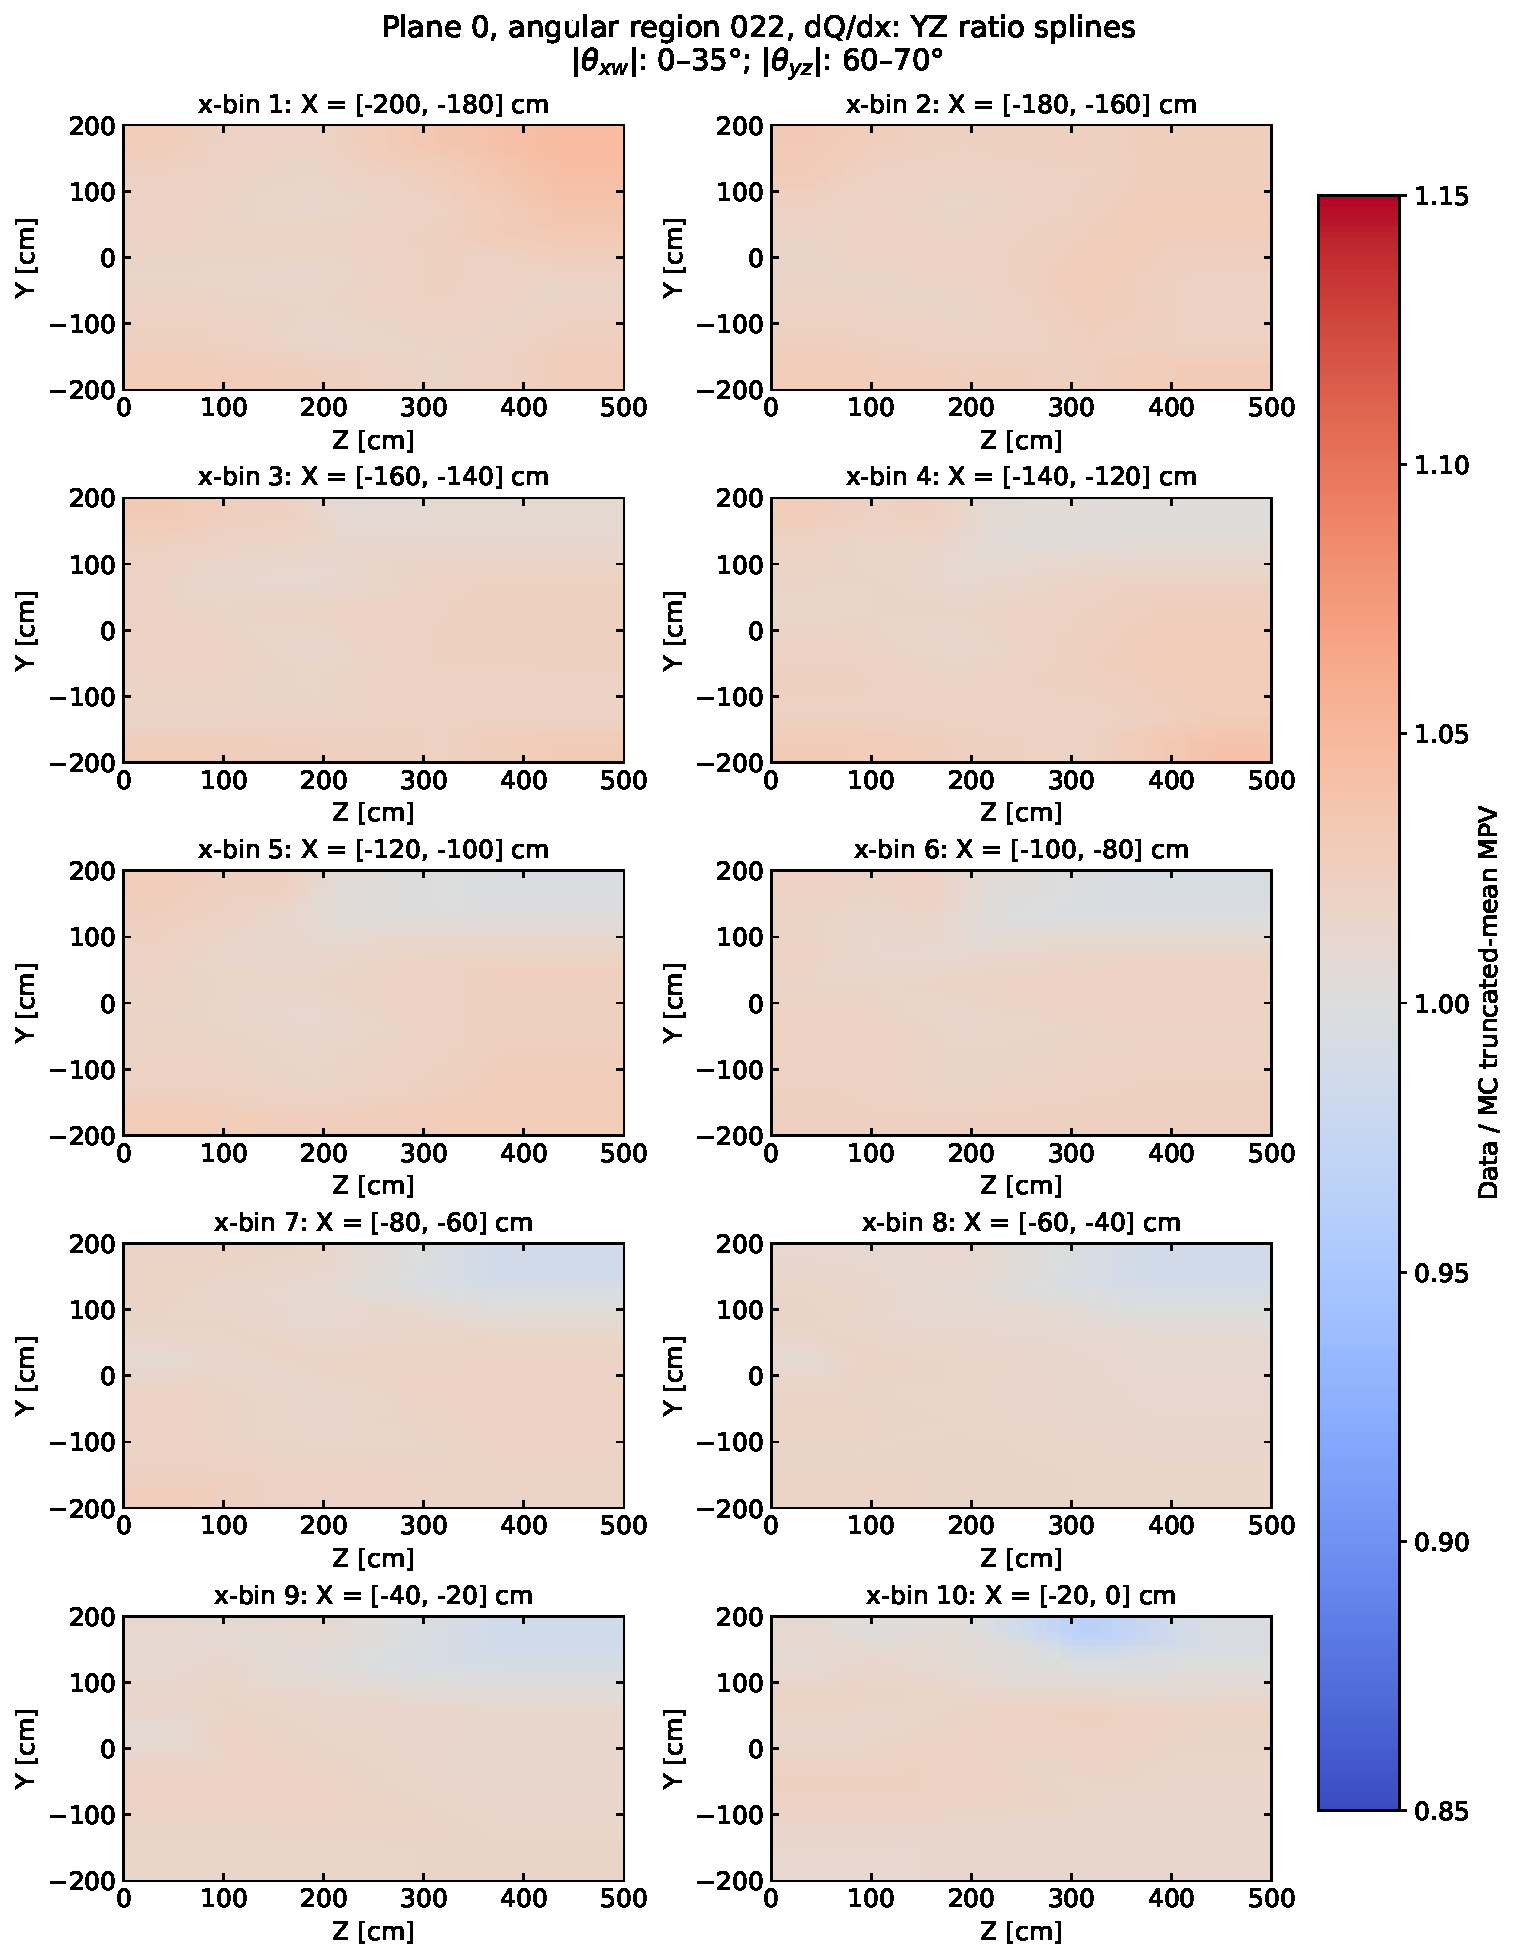
\includegraphics[width=\textwidth,height=0.80\textheight,keepaspectratio]{Figures/WireModXYZ/summary/plane0/anglebin_dq_plane0_region022_xyz_ratio_spline_summary_linear.pdf}
\caption{Plane 0, angular region 022: dQ/dx YZ data/MC ratio surfaces for all populated x-bins. The folded angular selection is $|\theta_{xw}|\in[0,35]^\circ$ and $|\theta_{yz}|\in[60,70]^\circ$.}
\label{fig:xyz_linear_dq_plane0_region022}
\end{figure}

\clearpage
\begin{figure}[H]
\centering
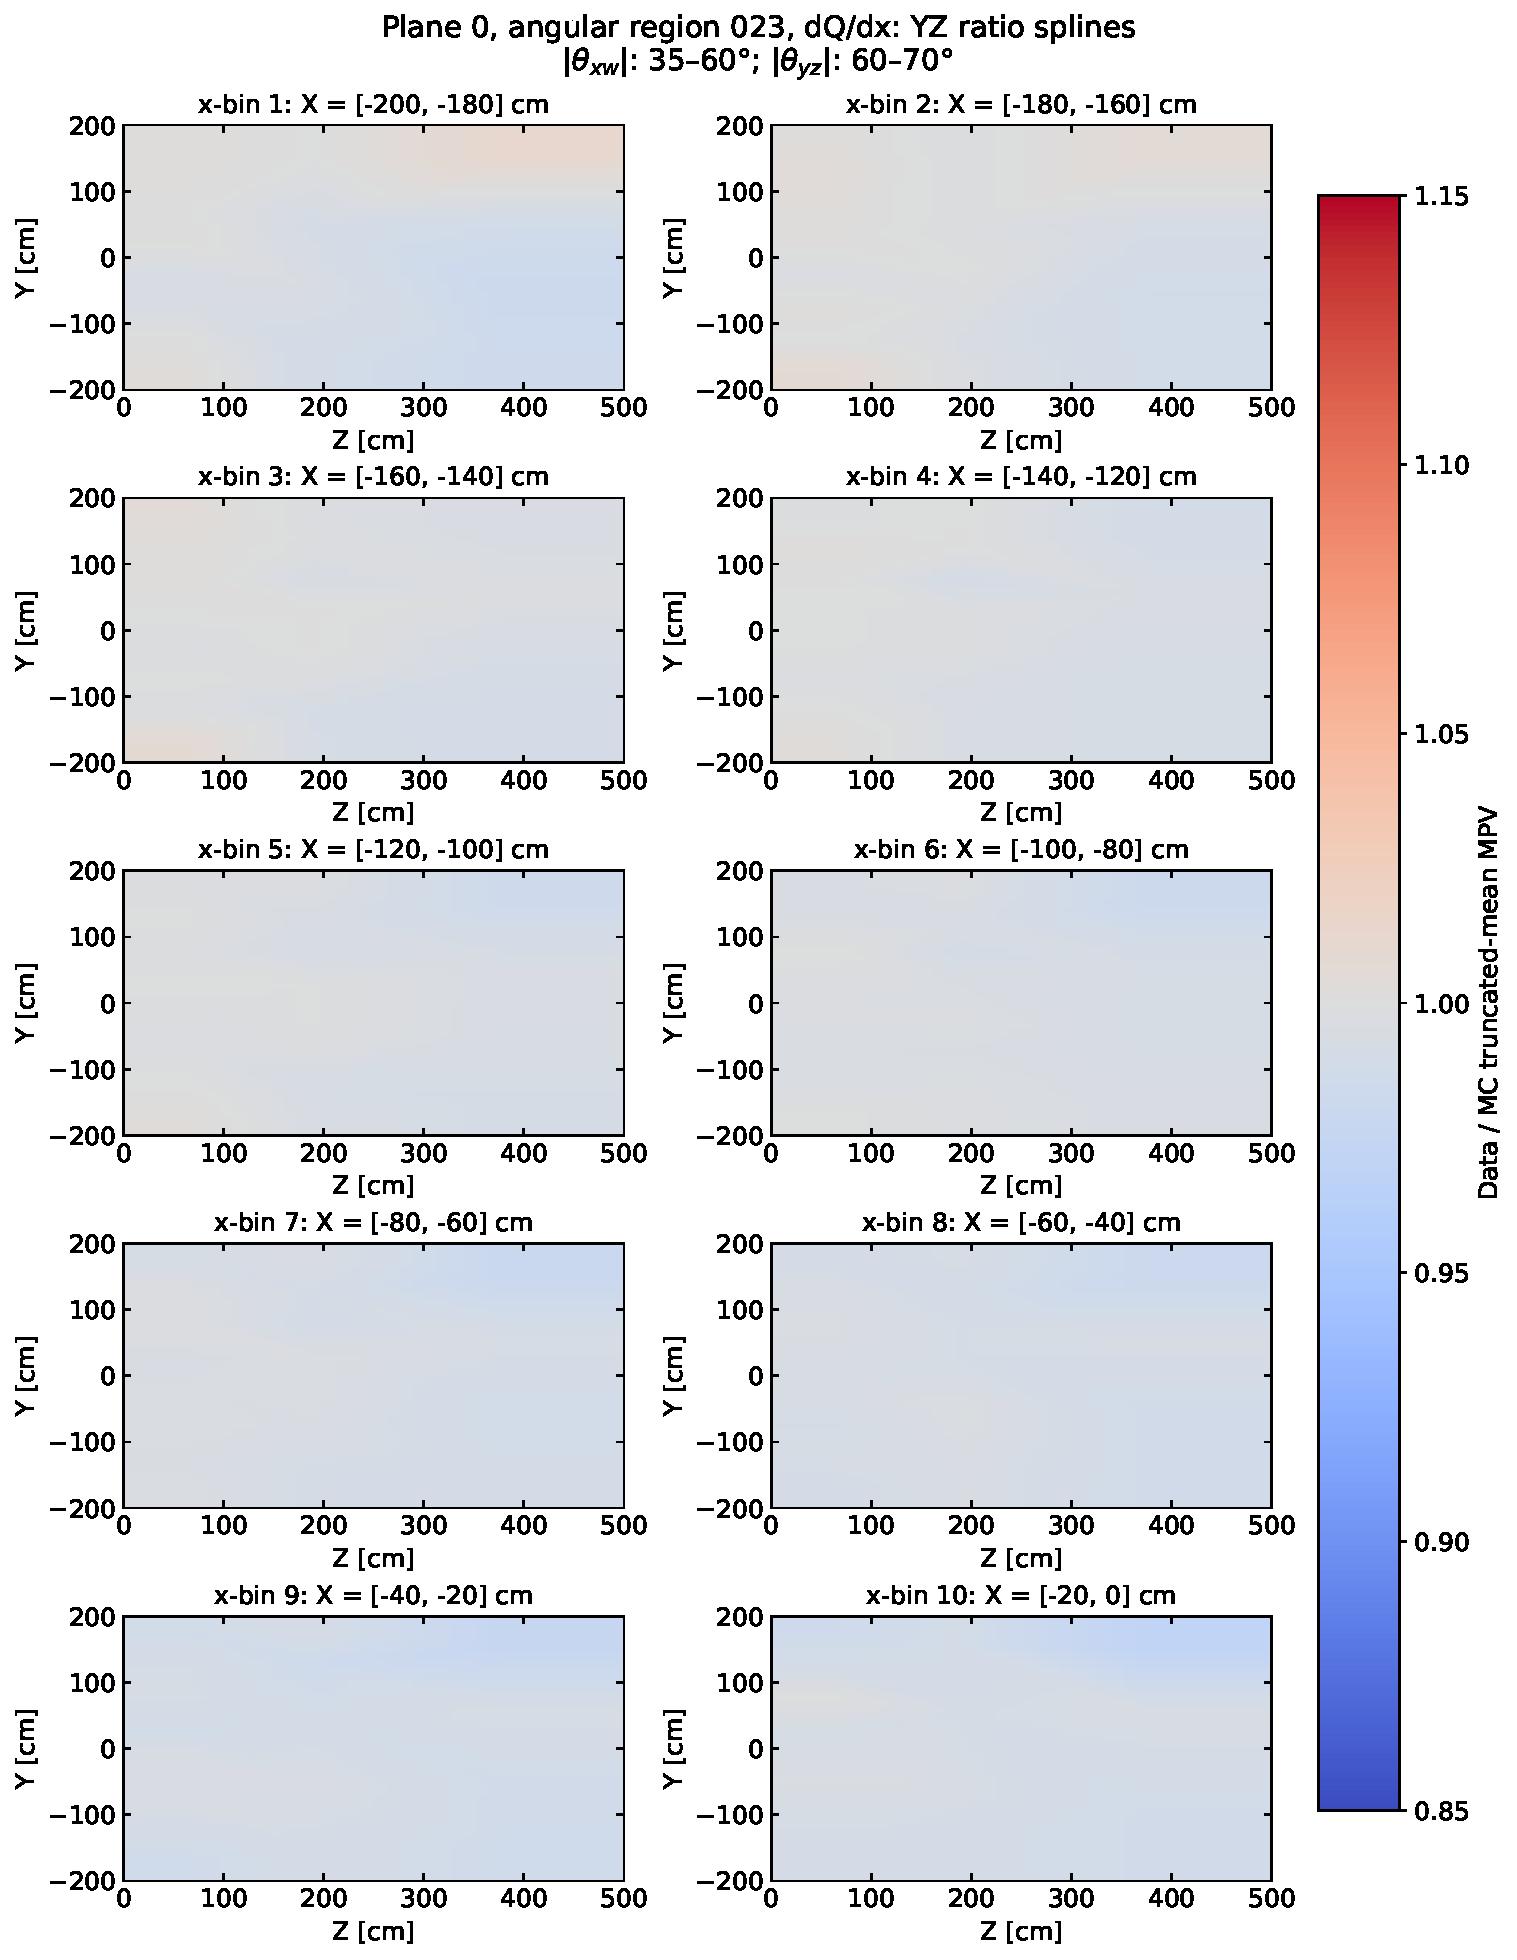
\includegraphics[width=\textwidth,height=0.80\textheight,keepaspectratio]{Figures/WireModXYZ/summary/plane0/anglebin_dq_plane0_region023_xyz_ratio_spline_summary_linear.pdf}
\caption{Plane 0, angular region 023: dQ/dx YZ data/MC ratio surfaces for all populated x-bins. The folded angular selection is $|\theta_{xw}|\in[35,60]^\circ$ and $|\theta_{yz}|\in[60,70]^\circ$.}
\label{fig:xyz_linear_dq_plane0_region023}
\end{figure}

\clearpage
\begin{figure}[H]
\centering
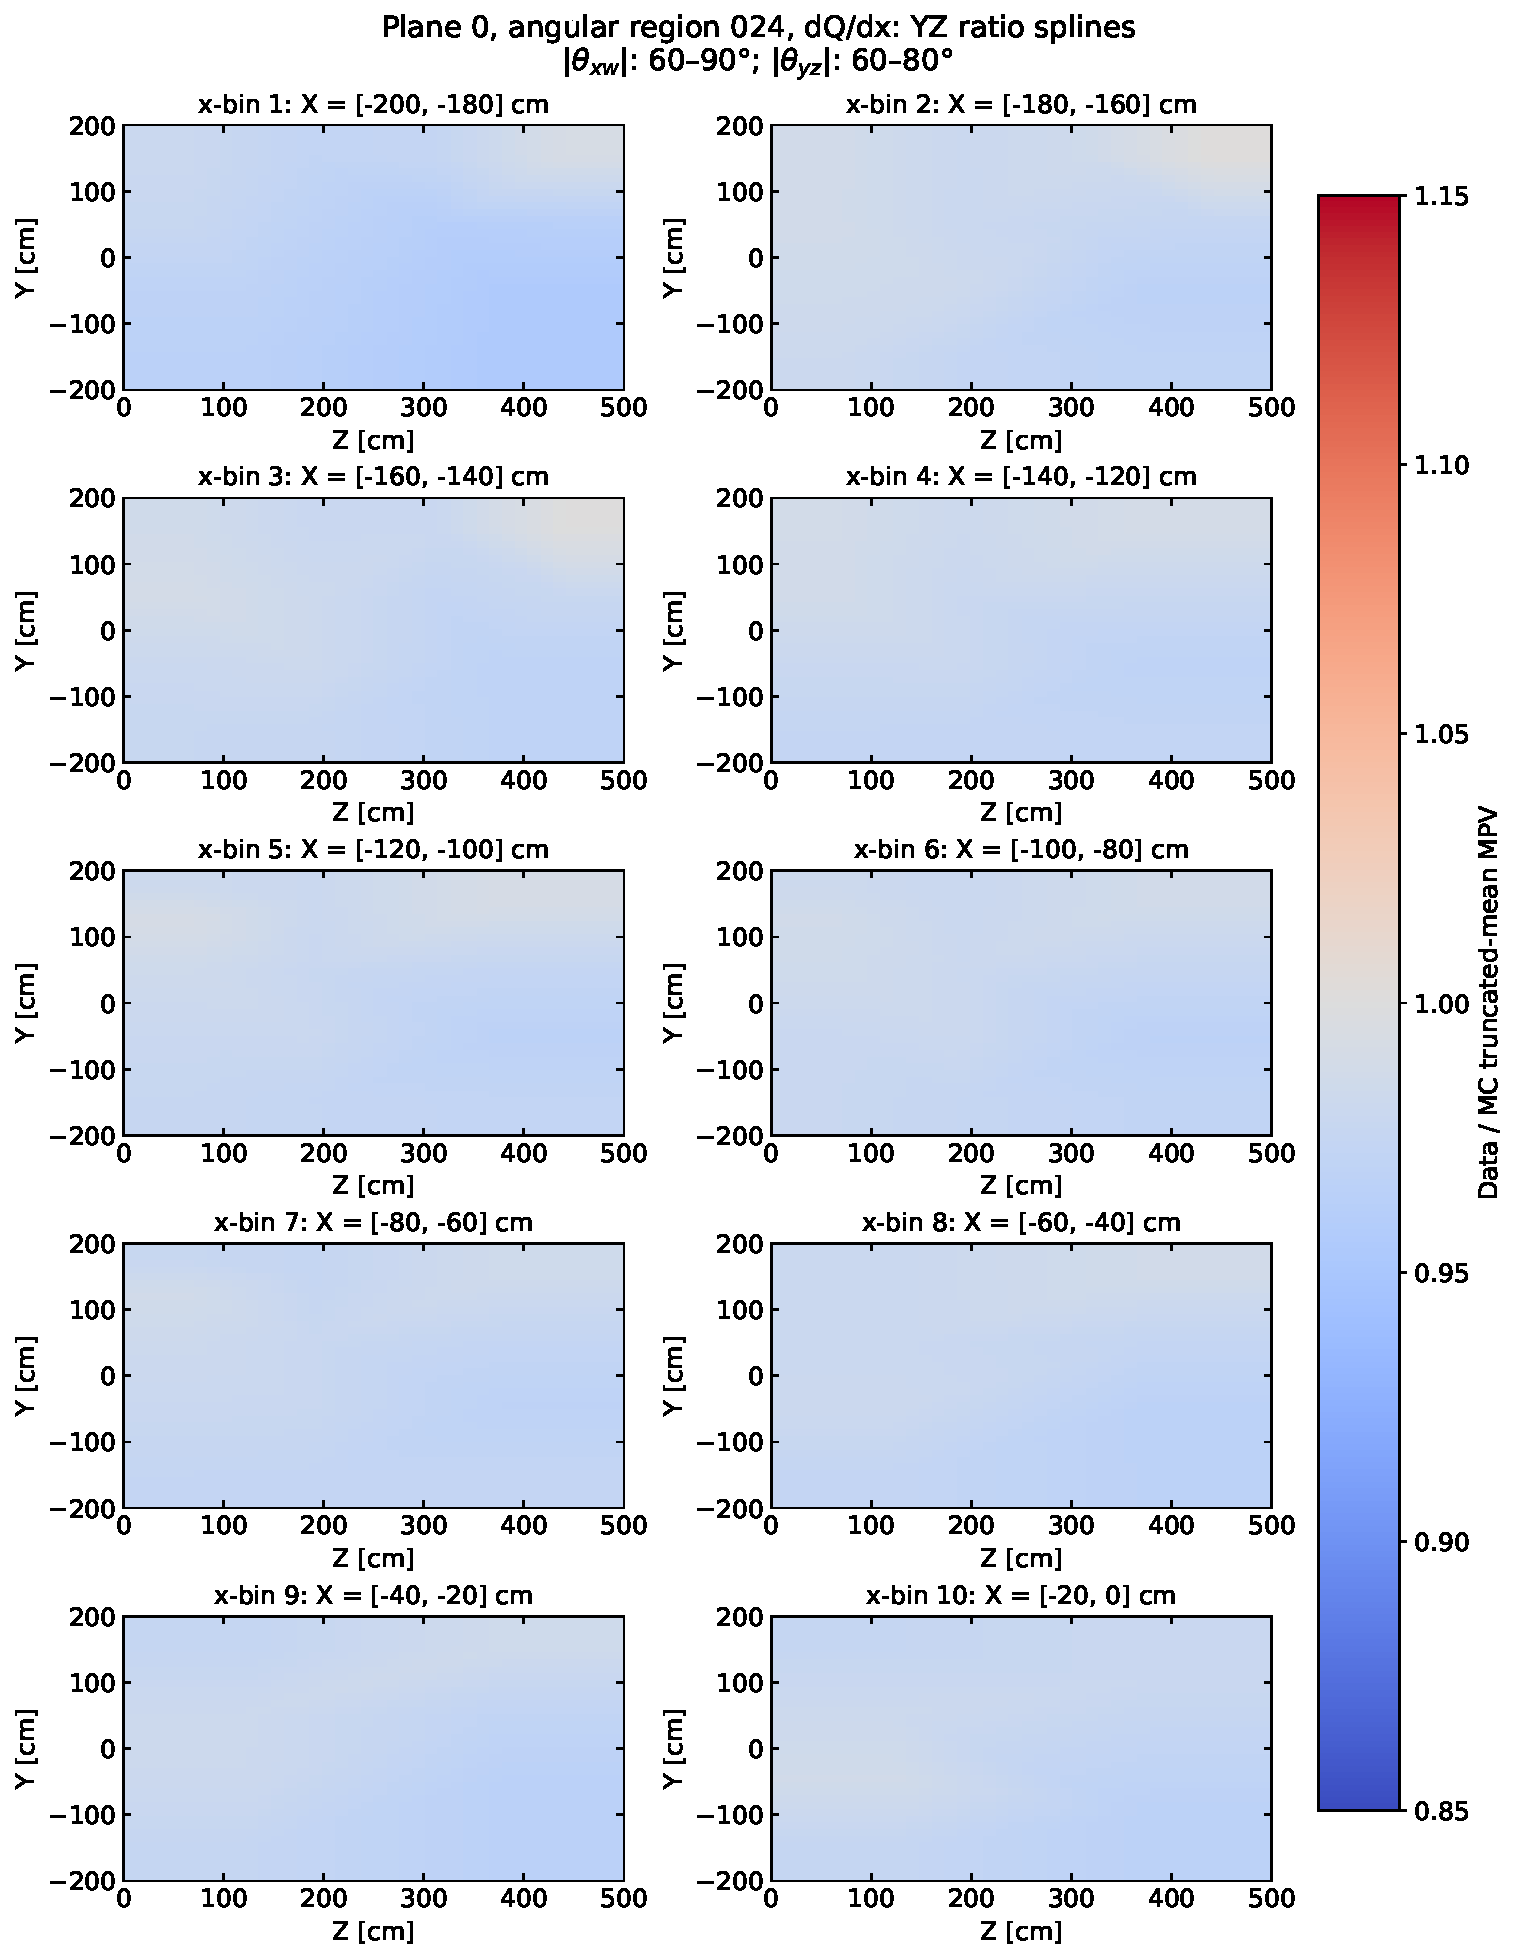
\includegraphics[width=\textwidth,height=0.80\textheight,keepaspectratio]{Figures/WireModXYZ/summary/plane0/anglebin_dq_plane0_region024_xyz_ratio_spline_summary_linear.pdf}
\caption{Plane 0, angular region 024: dQ/dx YZ data/MC ratio surfaces for all populated x-bins. The folded angular selection is $|\theta_{xw}|\in[60,90]^\circ$ and $|\theta_{yz}|\in[60,80]^\circ$.}
\label{fig:xyz_linear_dq_plane0_region024}
\end{figure}

\clearpage
\begin{figure}[H]
\centering
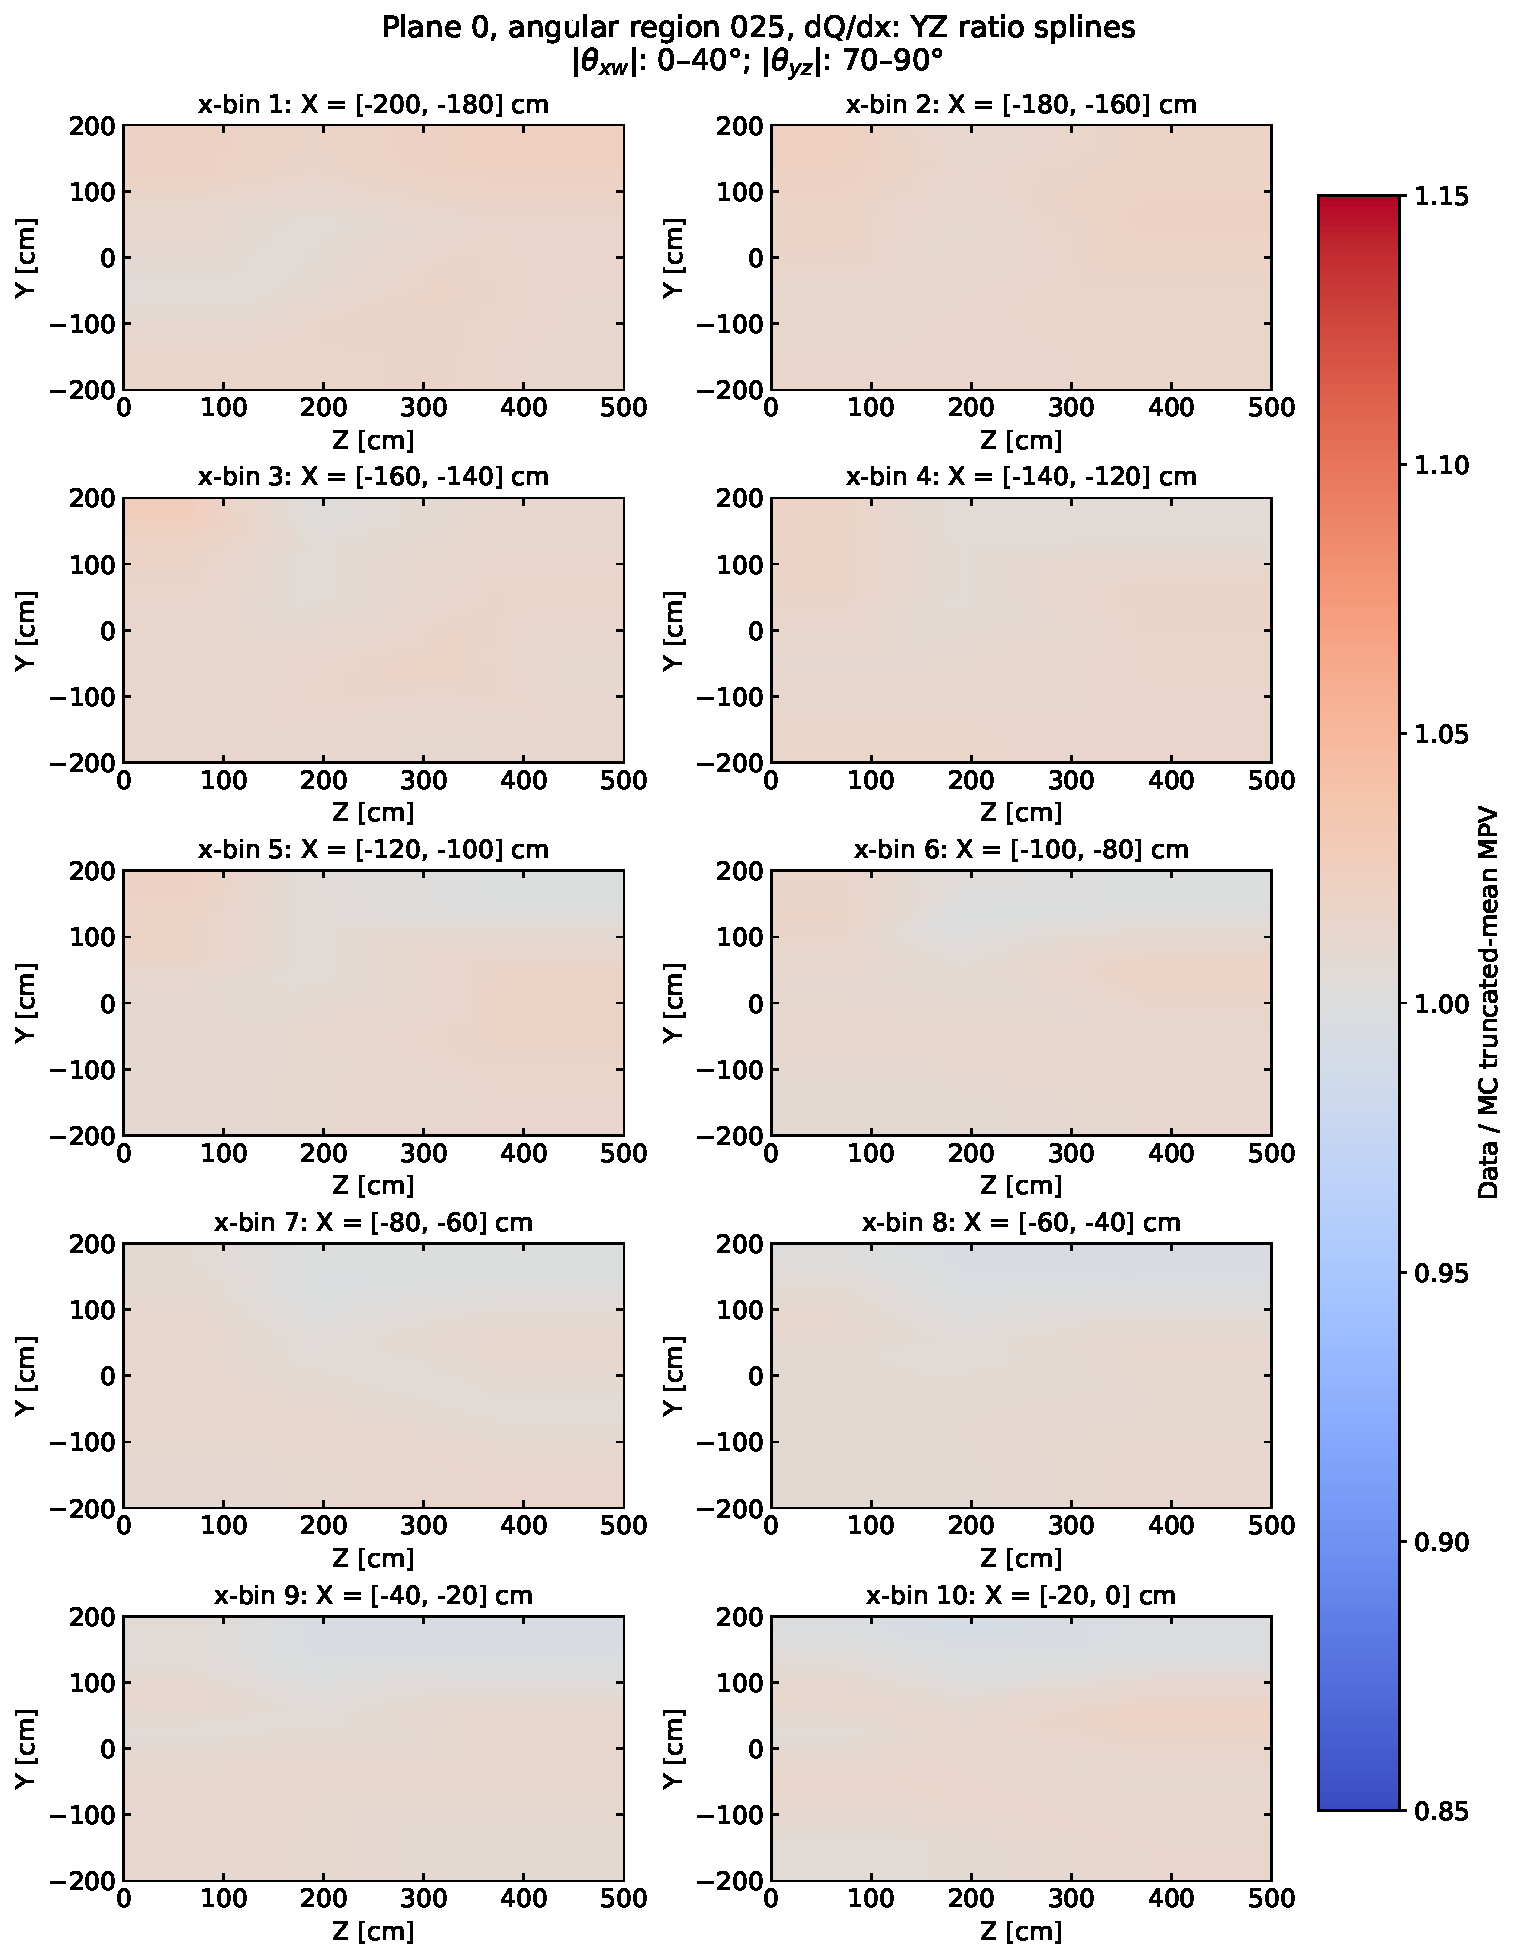
\includegraphics[width=\textwidth,height=0.80\textheight,keepaspectratio]{Figures/WireModXYZ/summary/plane0/anglebin_dq_plane0_region025_xyz_ratio_spline_summary_linear.pdf}
\caption{Plane 0, angular region 025: dQ/dx YZ data/MC ratio surfaces for all populated x-bins. The folded angular selection is $|\theta_{xw}|\in[0,40]^\circ$ and $|\theta_{yz}|\in[70,90]^\circ$.}
\label{fig:xyz_linear_dq_plane0_region025}
\end{figure}

\clearpage
\begin{figure}[H]
\centering
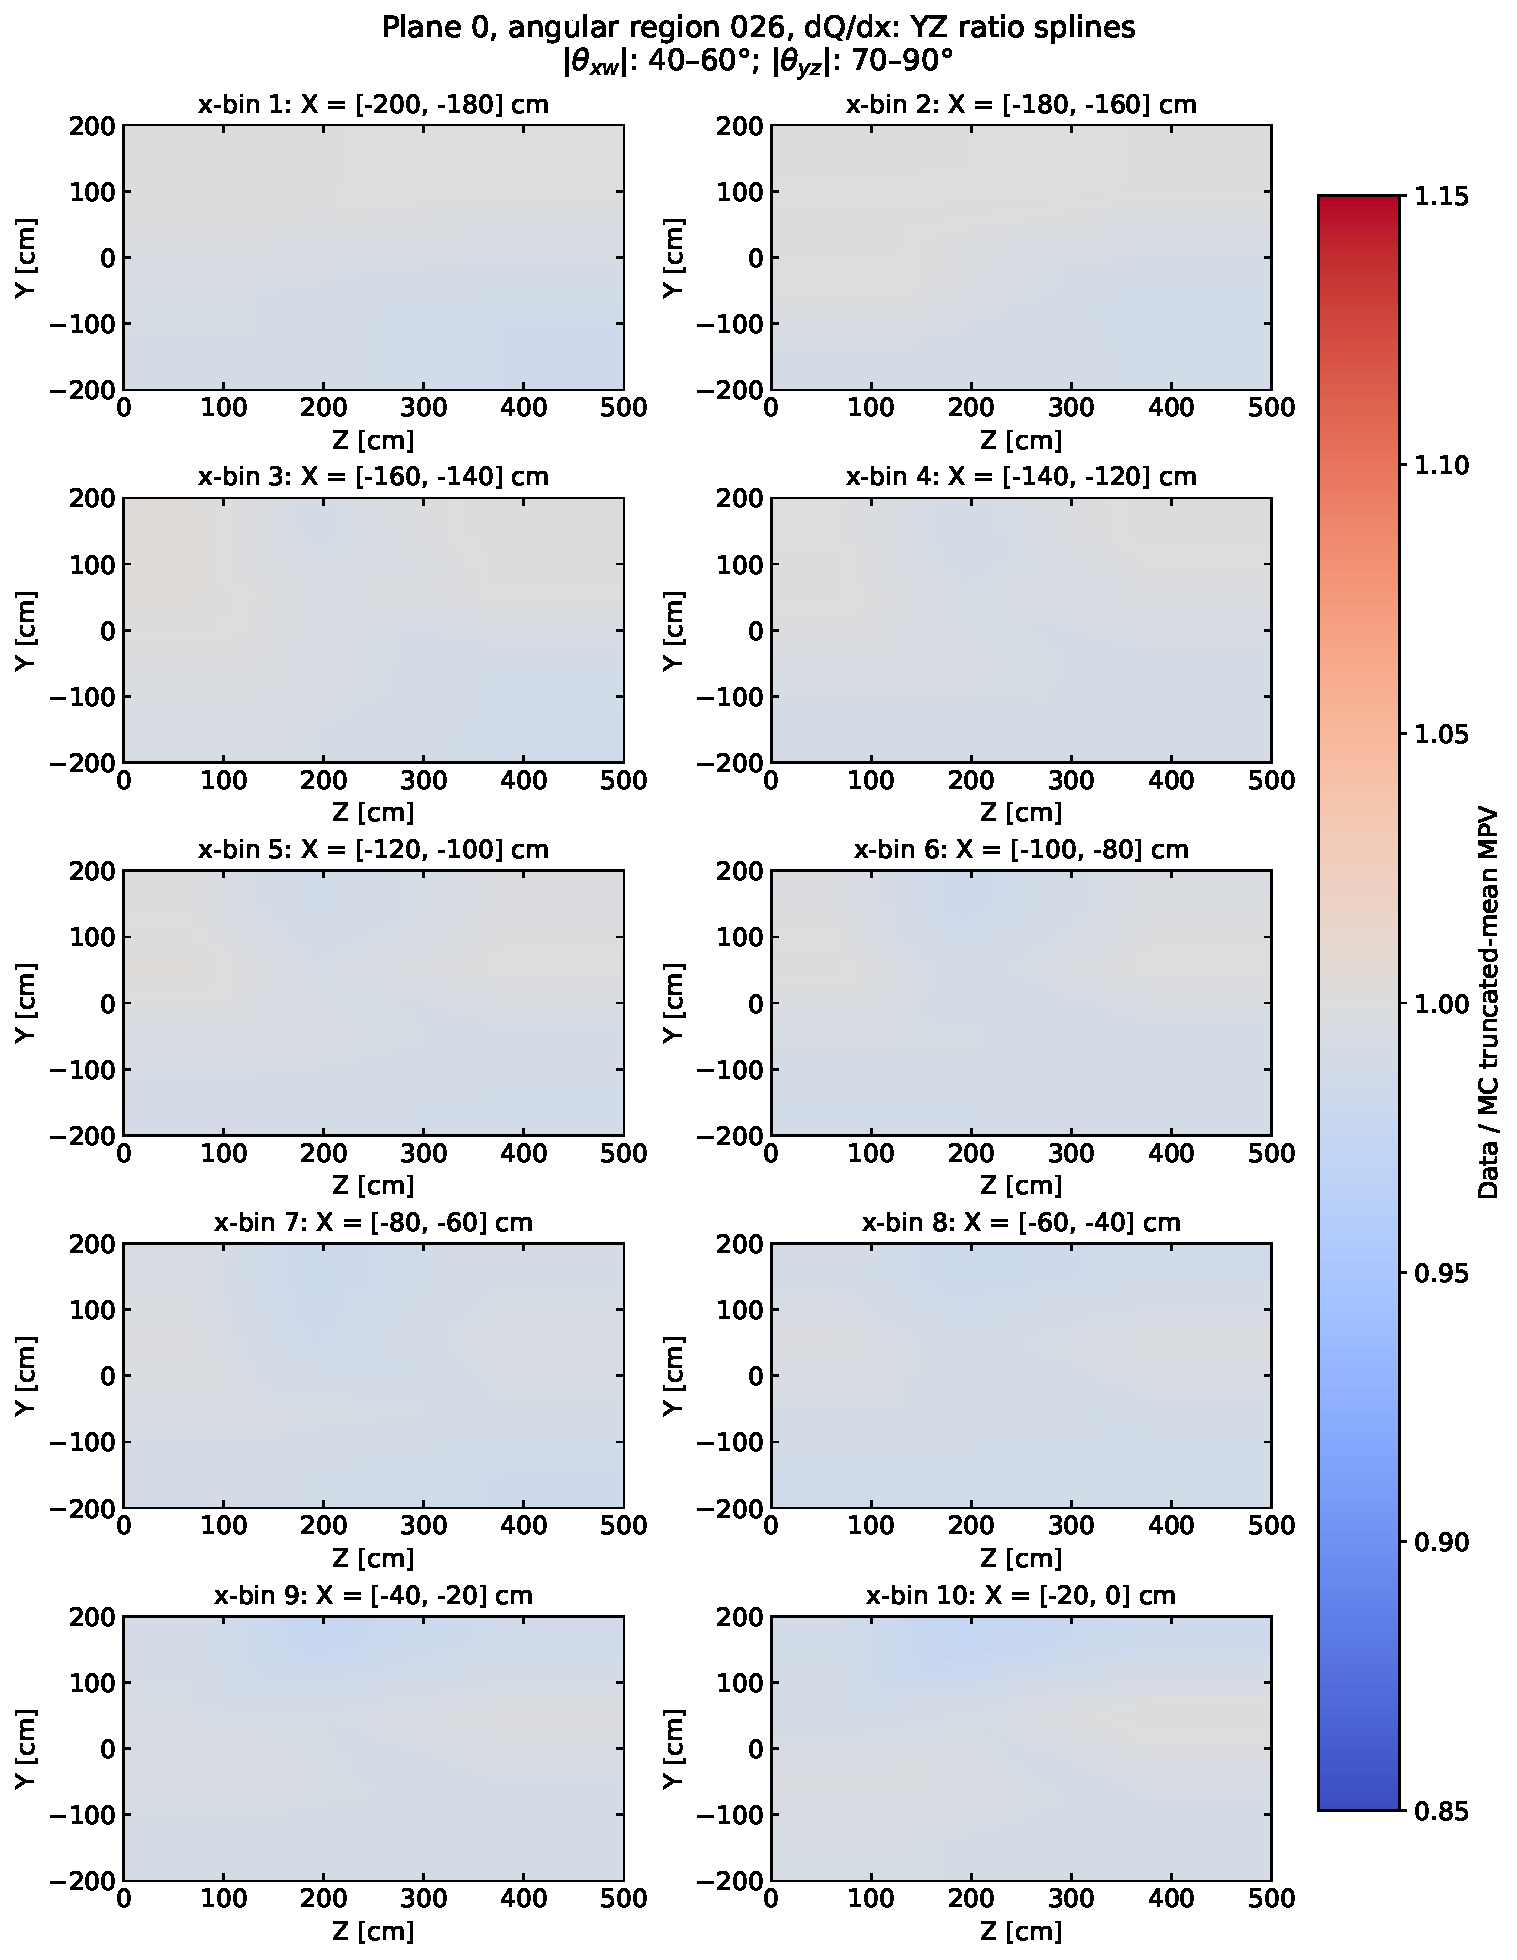
\includegraphics[width=\textwidth,height=0.80\textheight,keepaspectratio]{Figures/WireModXYZ/summary/plane0/anglebin_dq_plane0_region026_xyz_ratio_spline_summary_linear.pdf}
\caption{Plane 0, angular region 026: dQ/dx YZ data/MC ratio surfaces for all populated x-bins. The folded angular selection is $|\theta_{xw}|\in[40,60]^\circ$ and $|\theta_{yz}|\in[70,90]^\circ$.}
\label{fig:xyz_linear_dq_plane0_region026}
\end{figure}

\clearpage
\begin{figure}[H]
\centering
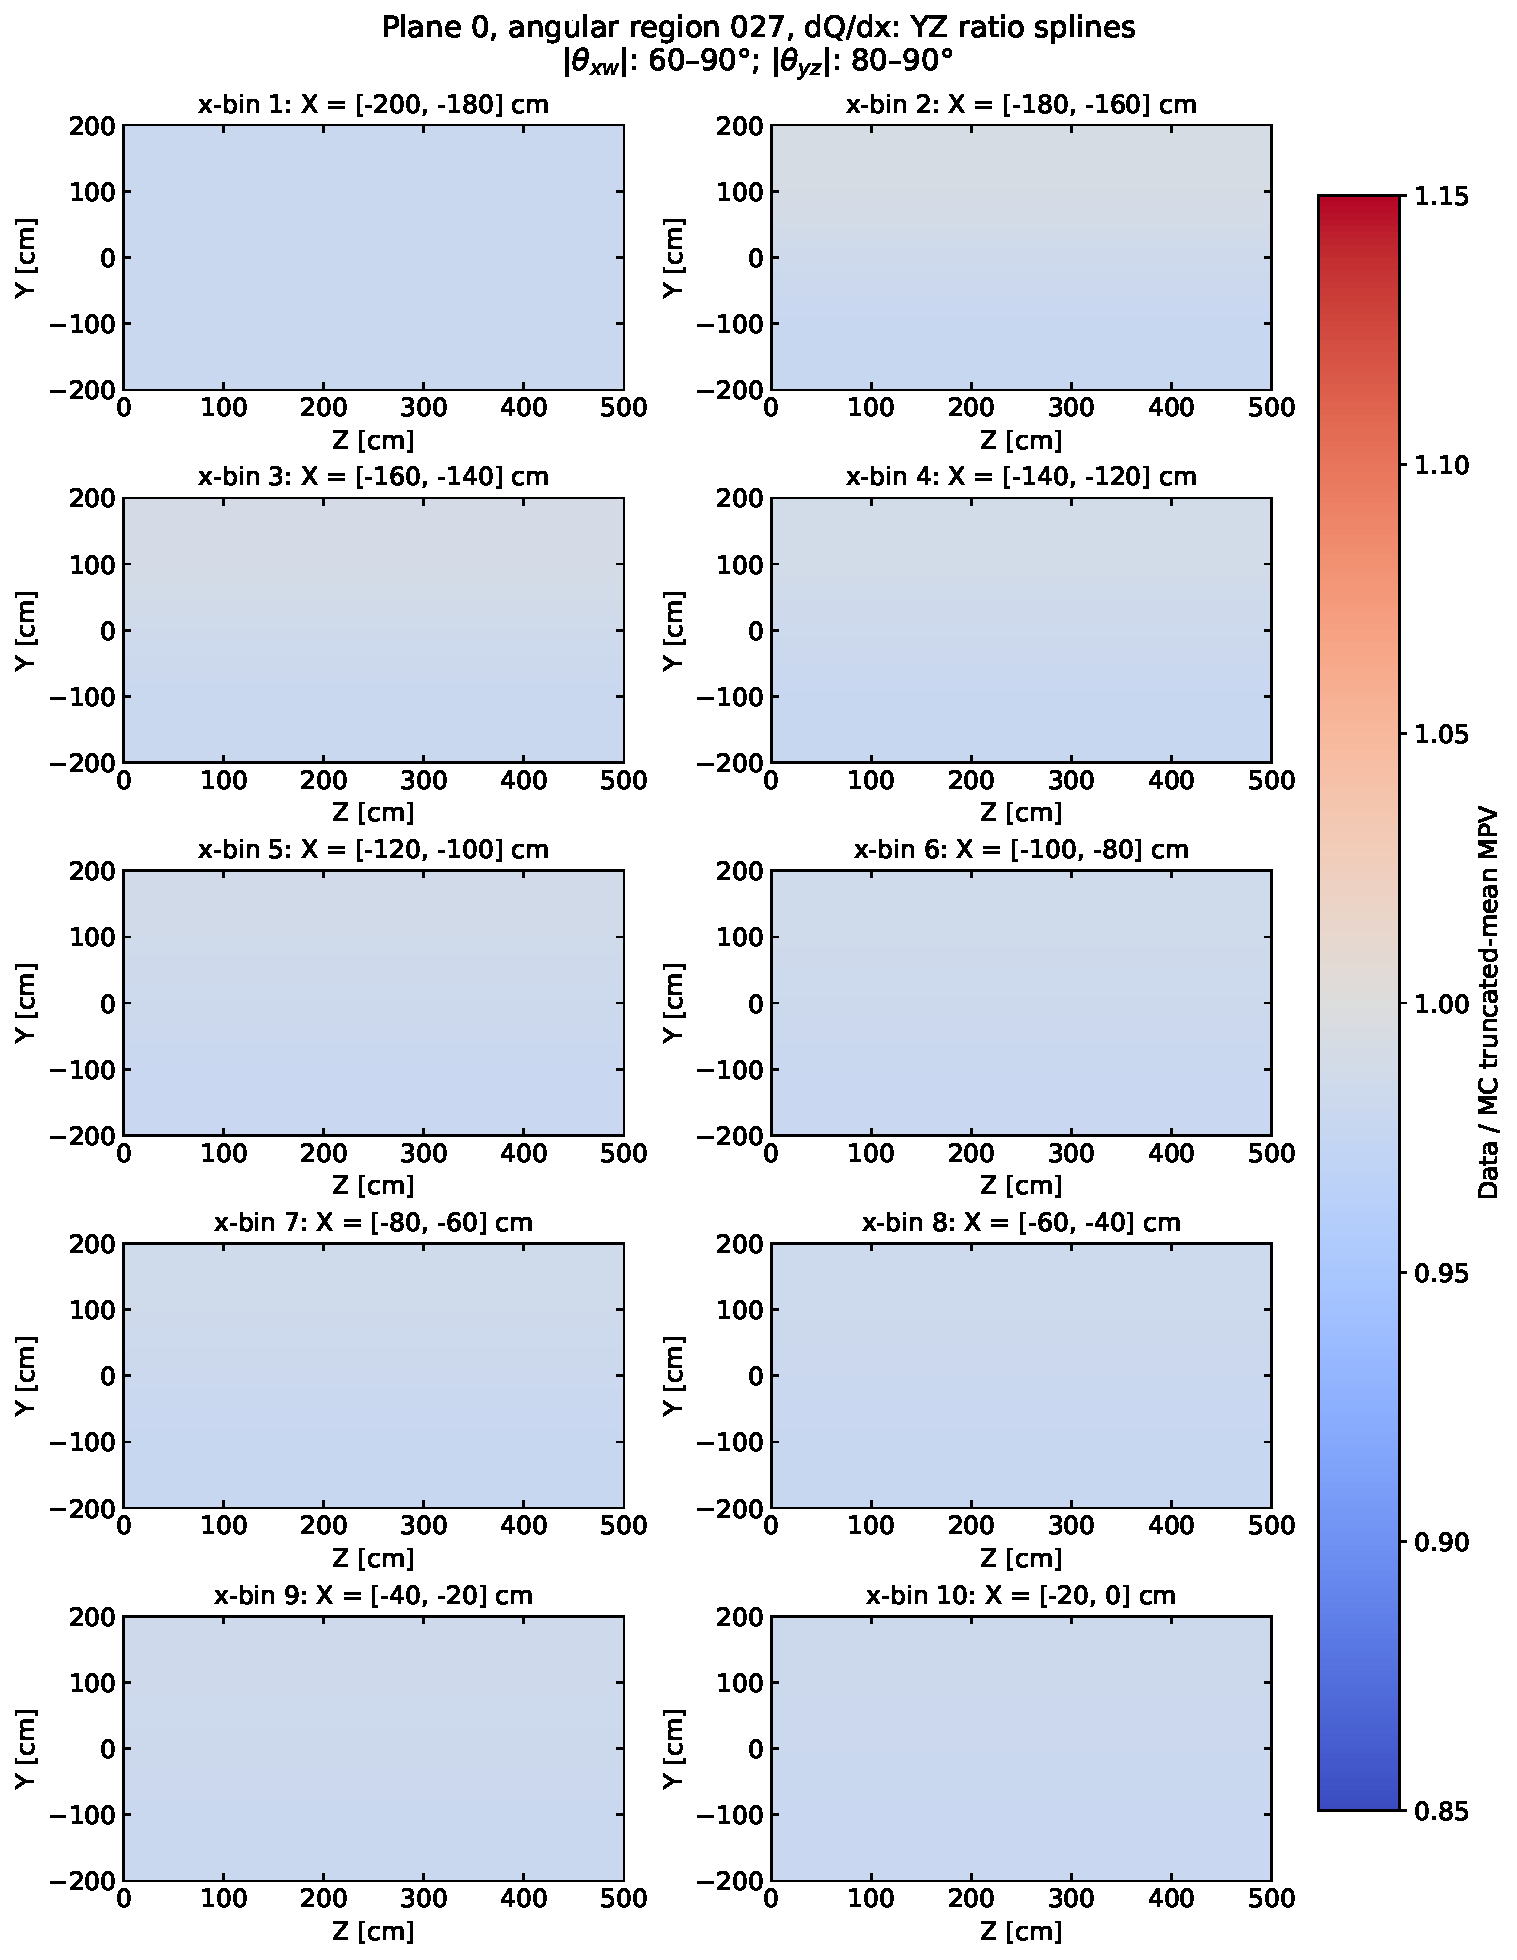
\includegraphics[width=\textwidth,height=0.80\textheight,keepaspectratio]{Figures/WireModXYZ/summary/plane0/anglebin_dq_plane0_region027_xyz_ratio_spline_summary_linear.pdf}
\caption{Plane 0, angular region 027: dQ/dx YZ data/MC ratio surfaces for all populated x-bins. The folded angular selection is $|\theta_{xw}|\in[60,90]^\circ$ and $|\theta_{yz}|\in[80,90]^\circ$.}
\label{fig:xyz_linear_dq_plane0_region027}
\end{figure}

